% This is a short template intended as a complement given
\documentclass[cleardoublepage=plain]{scrartcl}

% Package that allows more image formats to be included
\usepackage{graphicx}

% Package that allows international symbols
\usepackage[utf8x]{inputenc}

% Some packages containing math symbols and formatting
\usepackage{amsfonts}
\usepackage{amsmath}
\usepackage{amssymb}

% Package containing theorem, lemma and proof environments
\usepackage{amsthm}

% Package for easy inclusion of source code
\usepackage{verbatim}
\usepackage{alltt} 

% Package that adds automatic hyperlinks to your document
\usepackage[hyperindex=false]{hyperref}
\hypersetup{
plainpages=false,
colorlinks=false,
linkbordercolor={1 1 1}, % set to white
citebordercolor={1 1 1}, % set to white
urlbordercolor={1 1 1} 	 % set to white
} 

% Removes indentation when starting a new paragraph

\setlength{\parindent}{0pt}


\begin{document}

% Various important information about the document
\title{Robotics Project 2015 - CDT508\\ \Huge{SWARM}}
\author{\begin{tabular}{ll}
Peter Cederblad & pcd11001@student.mdh.se\\
Albin Barklund & abd11003@student.mdh.se\\
Roxanne Anderberg & rag11001@student.mdh.se\\
Ragnar Moberg & ragnar.morberg@gmail.com\\
Sudhangathan Bankarusamy & sby14001@student.mdh.se
\end{tabular}
\vspace*{0.5cm}\\ Märlardalens University \\ Västerås, Sweden}

\maketitle
\thispagestyle{empty} 
\newpage

% Removes page number from title page
\thispagestyle{empty} 



\section{Project introduction}
This year the project course has four different projects. ROARy, Butler, Swarm and a UAV project. 
All the students has been divided into pool groups with different specializations. Hardware, which developed all the electronics. Software, they developing and implemented code and simulations for different systems. Communications which worked with all type of communication e.g. how to communicate with the Naiad robot and how to control it. Mechanics they worked with the different structures and CAD programs for all projects.
The working hierarchy that has been used are four different project managers and four pool group leaders, with a different amount of workers. 
The project managers shall treat the pool groups as there was small consult companies and that the project leaders buy a service of them.
It is up to the group leader at every pool to distribute the work among his teammembers in order to achieve all the goals that the project managers has set up.

The purpose of this hierarchy is two folded. Firstly, reuse solutions between the projects in order not to invent the wheel all the time. Secondly, this hierarchy has the possibility to be more dynamic than if all students where locked in a small group working on a specific project.\\

This report will only address the swarm project.

The swarm project consists of two sides. One side consists of the old Naiad platform that was started to be developed in 2013 and the second side is swarm behavior. On the Naiad platform a light communication system for underwater purposes has started to be developed and a Wi-Fi solution for programming the robot has been installed, instead of the old ethernet cable.
A second robot has been started to be developed, which is called Naiads sister. The hull and motors are bought, but not assembled. A design for the hull to the new thrusters has been initiated.

The aim for the swarm behaviour side of the project has been on finding an Algorithm for shape forming, the project members has initiated  the implementation one. 

A new land based platform has been bought called kilobots. The purpose for using a land based platform instead of only the underwater platform, is that the school does not possess a large enough pool on the campus area that can fit more than one robot of the naiad type.

\subsection{The structure of the report}
The rest of the report has the following structure.
Section~\ref{sec:Goals}, contains a description of all the goals that has been set up for this project.

Secondly all the milestone for the different subsystems to be developed are located in section~\ref{sec:Milestones}.
Next section, section~\ref{sec:Requirements} lists all the specified requirements.

Section~\ref{sec:Planning}. The planning section shows the overall plan for this semester in tableform. For a more detailed description of the plan, open the file Swarm\_BIS.pod, which is located in the same dropbox map as this report.

Section~\ref{sec:NaiadOldSystem} contains an introduction of the subsystems that has been investigated during this year on the old Naiad platform. As well as an Quick starting guide for the Naiad.

Next section, section~\ref{sec:Naiadsister} describes the new platform that has starting to take form. In this section one can find the documentation of the new IMU card as well as future work on the platform.

Section~\ref{sec:WirelessCommunication} describes the need for a WiFi solution, what has happen on the wireless communication front this year, a short description on the configuration is also available and lastly there are behavioral-issues and future work.

Section~\ref{sec:Underwatercommunication} Underwater communication is described, this section is divided into two parts. Firstly there is the a section to del with the electronics that has been implemented. Secondly the communication between two computers using the developed electronic system solution.

Section~\ref{sec:Sonarcommunication} contains informations information on which students that will work on this during there masters thesis.

The swarm behavior section, section~\ref{sec:Swarmbehavior} is divided as dollows. A short introduction about what has been done and the purpose for this year. Secondly, it contains a description on the codes that has been implemented for the klobots. Thirdly a description of the Matlab code for the self-organizing coordinate system and the different start up codes in matlab for the next years students. Fourthly a summery of the S-DASH algorithm that still needs to be implemented is provided. and lastly  conclusions and future work.

Lastly the Section~\ref{App:appendix} contains all appendices for this project.


In this report the author's name for every subsection can be found in () after the subtitle. The author is responsible for the text until next name appear. The purpose of this is to make grading easier for the examining teacher.
The project leader, Peter Cederblad has putting it all together.
\newpage
% Creates table of contents
\tableofcontents
\newpage
\setcounter{page}{1}


\newpage
\section{Goals}\label{sec:Goals} 
For the Naiad platform the goals has been to build a second robot. Improve the power supply on the first robot. Go from ethernet cable to a wireless system for communication with the robot in surface mode. Also to develop two different underwater communication systems. One short range but fast with LED technology and one long range but more slow using sonar technology.


\section{Milestones}\label{sec:Milestones} 
Naiad
\begin{itemize}
  \item Current system up and running
  \item Wireless communcation using standard router
   \item Build new tail antenna
  \item New power supply
   \item Underwater light communication up and running
    \item Side sonar up and running
    \item Long range underwater communication up and running
\end{itemize}

Naiad sister
\begin{itemize}
\item Body
\item Build interial for electronics
\item Build all electronics
\item Communication interface
\item Light Communication between two robots
\end{itemize}

Wireless communication
\begin{itemize}
\item Specification
\item Underwater test
\item Tail Antenna complete
\end{itemize}

Light communication system
\begin{itemize}
\item Specification
\item Land test, Prototype solution
\item Underwater test, working solution
\end{itemize}

Swarm behavior
\begin{itemize}
\item Self-coordinate system
\item S-DASH in Matlab
\item S-DASH on kilobots
\end{itemize}



\section{Requirements}\label{sec:Requirements} 
Naiad platform new power supply, ring design.% Kolla med Albin
The wireless router shall be small enough to fit inside the current platform.
The wireless router must be able to work in the current system without major changes to the power plant.
The antenna for the wireless communication system shall resemble a stingray tail.
The antenna shall be stiff.
The antenna's length shall be 30 procent of the length of the Naiad platform.
The toolplate shall be able to mount the side sonars developed by DeepVisionAB in Lindköping.
The toolplate shall be build of the same material used on the current platform.
The underwater light communication shall be able to work in pool water with a range of 100 m.
The long range underwater communication system 





\section{Planning}\label{sec:Planning} 
The plan for the the Naiad platform this fall has been
\begin{itemize}
\item Current system knowledge
\item Current system up and running
\item Test: water leakproof
\item Test: Old system dive
\end{itemize}

The plan for development of the wireless communication
\begin{itemize}
\item Specification for wireless communication
\item Develop wireless communication
\item Test: Wireless communication system
\item Verification and validation on the improved Naiad
\item  Build tail antenna
\end{itemize}

The plan for side sonar overlapping with stereovision
\begin{itemize}
\item Specification of sonar element for overlapping image with stereo vision
\item Order hardware for sonar element
\item Design
\item Build sonar holder for Naiad
\item Implemention: Software overlapping between sonar and Gimme 2
\item Test: Sonar and Camera in a big pool
\item Verification and validation
\end{itemize}

The plan for Naiads sister
\begin{itemize}
\item Specification on Naiads sister
\item Design
\item Buy hull and motors
\item Build interial for the electronics
\item Build the electronics
\item Implement new software
\item Integrate subsystems
\item Test: Water leakage proof
\item Test: Naiads sister dive test
\end{itemize}

The plan for the light communication system
\begin{itemize}
\item Specification light communication
\item Design light communication
\item Develop light communication system
\item Test: Blink light communication
\item Verification and validation
\end{itemize}

The plan for the long range communication system
\begin{itemize}
\item Specification for sonar communication
\item Design sonar communication system
\item Develop sonar communication
\item Test: Sonar communication
\item Verification and validation
\end{itemize}

The plan for the landbased platform
\begin{itemize}
\item Read state of the art
\item Specification on the landbased robot platform
\item Search for landbased robot platforms
\item Order landbased robot platform
\item Hands on sytem knowledge on the purchased system
\end{itemize}

The plan for the swarm behavior
\begin{itemize}
\item Read state of the art
\item Design: Information repressentation
\item Design: Path Planning
\item Develop algoriths for swar behavior
\item Development of simulator
\item Implementation on landbased platforms(Kilobots)
\item Test on AUV scenarios
\item Verification and validation for AUV scenario 1
\item Verification and validation for AUV scenario 2
\item Test on landbased platforms()
\item Verification and validation on landbased platform
\end{itemize}

The plan for presentation
\begin{itemize}
\item Result of landbased swarm system
\item simulation result for AUV scenario 1 and 2
\item Result on the light communication system
\end{itemize}

Chrismas holiday
Report writing and time for completion



\section{Naiad old system}
\label{sec:NaiadOldSystem}


\subsection{Introduction (Peter Cederblad)}
For this year a light communication system has started to take place and a wi-fi solution has been implemented. There has also been work done in making a new antenna for the wi-fi connection.
We where also given the task at looking into how to integrate a side-sonar on the Naiad that in order to overlap the sonar picture with the stereo vision that is already onboard the platform. Not much work has taken place here, a few students went down to Lindköping and meet the company that are developing this kind of solutions. The companys name is Deep Vision AB.  There has also been work in manufacturing a new tool plate in order to be able to use the side-scan system.

All systems that has been developed for the Naiad is also for the sister robot and will not be written about here. Instead all systems has there own section in this report.
The mechanics group has written one report that covers all there work during this fall, it can be found in the appendix ~\ref{App:MechanicsReport}


\subsection{Software Guide to Quick Starting NAIAD - Sudhangathan Bankarusamy(This subsection)}
The NAIAD is mainly controlled by a Beagle Bone Black(BBB) running Ubuntu 12.04. Given below is a series of steps that will start the thrusters with a mission. Before starting with the steps below, care should be taken so that NAIAD is powered-up using 22.5V power source, both kill and mission switch is plugged in its respective slots, the UL(user led) LEDs on all CAN cards must be flashing. Also a computer, preferably a laptop should be connected to the network switch, using a LAN cable or connected to the wifi access point as explained in later sections, so that a network connection from the computer to the BBB exists. The IP address on the computer should be manually set to 192.168.1.10(192.168.1.xxx).

\begin{enumerate}
  \item From the the computer using a terminal type: \\ssh ubuntu@192.168.1.1 \\for password enter "ubuntu"
  \item type:\\cd BBB/
  \item type: \\sudo system.sh run \\in this step the all the programs necessary for the mission are running
  \item In order for the thrusters to start, pull out the mission switch.\\At this point the thrusters should start working
  \item Pulling out the kill switch will stop the mission and the mission will be restarted once the kill switch and mission switch are put back.
  \item type:\\sudo system.sh kill \\This will stop all programs
%  \item The third etc \ldots
\end{enumerate}

\subsection{Conclusions (Peter Cederblad)}
There are a few systems that has begun to be implemented. However it is obvious that when a project like Naiad, that has a few years on the neck the students are starting to lose their interest in it. Especially when there are a lot of other projects around them that are newer.

\subsection{Future work}
On the Naiad platform there are several things that needs to be improved.
\begin{itemize}
\item Light communication system
\item Sonar communication system
\item Side-scan with stereo vision
\item Wi-Fi antenna
\item Toolplate
\end{itemize}
These are all subsystems that still has lots of work.



\section{Naiad sister}
\label{sec:Naiadsister}
\subsection{Introduction}
The second Naiad has begun to take place. At least the major part of the hull and the thrusters has arrived to the school. Unlockely there has not been so much time in order to assemble the hull or the thruster hulls. A new power supply has been discussed, but the students in charge of that has not documented it. The same for the thruster hulls. But an new IMU card has been made to the new IMU.

\subsection{IMU card - Roxanne Anderberg}
\subsubsection{Description and Requirements}
For measuring yaw, pitch and roll, Naiad uses an inertial measurement unit. In this case VN-100 Rugged~\cite{rugged} from Vectornav~\cite{vectornav}.
VN-100 Rugged can communicate through TTL or RS-232 and since Naiad's CAN card has UART the decision of making a UART RS-232 adapter was made. Luckily there are transceivers on the market for just that kind of adaption.


\subsubsection{Design and Interface}
For making an UART RS-232 adapter you only need a transceiver~\cite{max232} and the matching capacitors for that transceiver. On this card I have also made pinouts that have been carefully measured so the card can match the CAN cards perfectly as an extension card. The second and final version of the IMU card have shorter sides so that the communication group can reach the pins for the debugging on the CAN card without having to remove the IMU card. There also been added test points for testing the transceiver.



\subsubsection{Testing}
For testing the transceiver to make sure it is not broken I used a few steps found on a forum~\cite{test}:
"Troubleshooting this IC is not difficult. 
Power up the MAX232 and check voltage across supply pins to insure correct voltage input. 
The following two tests check each "TTL in - RS232 out" converter. 
Put 0 volts into pins 10 and 11, then check pins 7 and 14. Should have about 10 volts output on each. 
Put 5 volts into pins 10 and 11, then check pins 7 and 14 again. Should have about -10 volts output on each. 
If that succeeded, then check each "RS232 in - TTL out" converter. Connect pin 7 to pin8. Connect pin 13 to pin 14. This will be a "loopback test". 
Put 0 volts into pins 10 and 11, then check pins 9 and 12. Should have about .6 volts output. 
Put 5 volts into pins 10 and 11, then check pins 9 and 12 again. Should have about 4.5 volts output."\\
\\
For testing the circuit you can use an oscilloscope on the UART pins and the RS-232 pins to make sure that they receive/send the right data.
%lägga till något om hur fyrkantsvågen ska se ut här??


\subsubsection{Using the system}
The card is very much plug and play, but before using the IMU it is very importing to read the manual. There suppose to be manuals in the school but one can also find them online~\cite{manual}. 
%lägga till något om tutorial??


\subsubsection{Future Work for IMU card}
The card that has been printed is not a card that should be used because it has some faults. Find a good MAX232, there is many versions. Test it on a breadboard first to see if the direction of the capacitors are the same as the datasheet. For printing out in school, make sure to have the traces to the hole mounted components on the other side of the card. Will be a bit hard to solder otherwise.
Also future work is the cabeling between the IMU and the PCB. The Harwin connector, see table~\ref{BOM}, is very expensive and difficult to attach. The IMU must have the female version but for the card I would recommend another type of connector. 



\subsection{Conclusions(Peter Cederblad)}
There are a lot here that can be improved from the first robot. No need to rush it and make bad decisions.

\subsection{Future work Naiad sister}
Everything.



\section{Wireless Communication}
\label{sec:WirelessCommunication}


\subsection{The need for the WiFi module(Sudhangathan Bankarusamy)}
The cables used for the NAIAD AUV had limiting issues such as the range, drag due to the cable running through water, which also adds up energy expenditure. Moreover the cables were an alternative to the limiting under water wireless technology issues. 
The Wi-Fi router is a starting point for trying various wireless technologies. 
\subsection{Network configuration}


Configuration without wireless router was a simple star network where a gigabit switch is used and all devices can connect to it using a LAN cable.
In the configuration with the Wi-Fi device(an ASUS WL-330n) is used in 'access-point' mode. This access point is used as a gateway between wired and wireless devices. The DHCP range in it's configuration page is set to 192.168.1.3 to 192.168.1.99.\\
The IP address of BBB remains as 192.168.1.1 and that of the access-point is set to 192.168.1.2.

\subsection{Behaviour and the issue}
The router performed well as expected, but only as long as the NAIAD AUV is not under the water surface. As the Wi-Fi signal deteriorates heavily through water, the connection is immediately dropped when the AUV is submerged in water.


\subsection{Future work}
\textbf{Implement OpenVLC} - OpenVLC is an embedded framework for visible light communication. It has the complete software stack, from MAC to application layer libraries. OpenVLC can run in Linux on BeagleBoard. After setting up OpenVLC, an interface VLC0 is created through which we can send/receive ethernet data. The physical media is light through the air. The prototype setup is further discussed in Underwater Light Communication section.\\
\textbf{SONAR} - Sonar is the most used technology for under water communication. It has been shown to perform well for long distance under water communication.\\



\section{Underwater communication}
\label{sec:Underwatercommunication}

%\subsection{Introduction}



\subsection{Electronic part (Albin Barklund)}
\subsubsection{Description}
The light communication module is a wireless data link for short distance underwater communication between autonomous underwater vehicles (AUVs). It consists of a receiver and transmitter which utilizes power LEDs and photoresistors to send and receive data.\\\\
Bear in mind that no actual solution have been implemented and this document only summaries a couple of experiments which where conducted to prove or disprove the hypothesis in section \ref{sec:hypothesis}.
\subsubsection{Requirements}
\label{sec:req}
\begin{tabular}{l l}
Range: & 2 - 3m\\
Data rate: & 1 kbit/s\\
Input data signal: & 5V\\
Medium: & water\\
\end{tabular}\\


\begin{figure}[h]
\centering
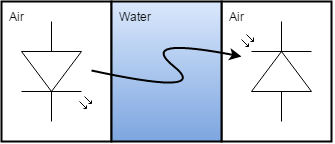
\includegraphics[width=0.5\textwidth]{medium}
\caption{Signal transistion through mediums}
\label{fig:con}
\end{figure}


\subsubsection{Hypothesis}
\label{sec:hypothesis}
With the use of power LEDs and photodiodes it is possible to create a wireless data link for underwater communication that modulates bits simply letting an asynchronous data signal control a LED which fulfill the requirements in section \ref{sec:req}


\subsubsection{Design and interface}
\textbf{Transmitter}\\
The transmitter takes an asynchronous data signal as input. The driver stage then inverts and amplifies the signal which then drives the LED. If the signal is high then the LED is turned off and if the signal is low then the LED is turned on.

\begin{figure}[h]
\centering
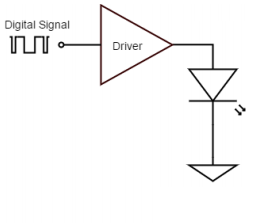
\includegraphics[width=0.4\textwidth]{trans}
\caption{The transmitter}
\label{fig:trans}
\end{figure}

 
 \textbf{Receiver}\\
The flashing pulses from the LED excites the photodiode and converts the light into current. The current is then converted to a voltage and passed through an amplifier. Since the signal to noise ratio is very low both ambient noise and fluorescent light needs to be filtered out from the signal which is accomplished by the high pass filter. Finally the signal gets reconstructed through a schmitt trigger.

\begin{figure}[h]
\centering
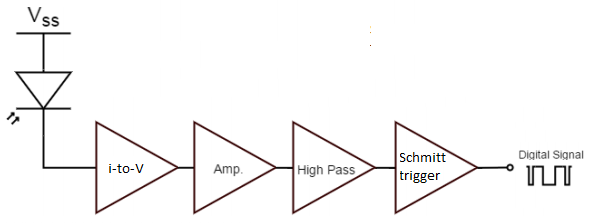
\includegraphics[width=0.8\textwidth]{rec}
\caption{The receiver}
\label{fig:rec}
\end{figure}


\newpage

\subsubsection{Test and simulation results}
The system has proven capable of transmitting asynchronous data with a baud rate of 4800 within a range of 2 meters on land. If a rectangular cointaner filled with water were put in between the transmitter and receiver the range decreasesed to 1 meter. \\\\
The transmission only succeeded if data were sent continuously. If a short break would occur in the continues data stream it takes approximately 20 bytes before the receiver starts outputing valid data again.

\begin{figure}[h]
\centering
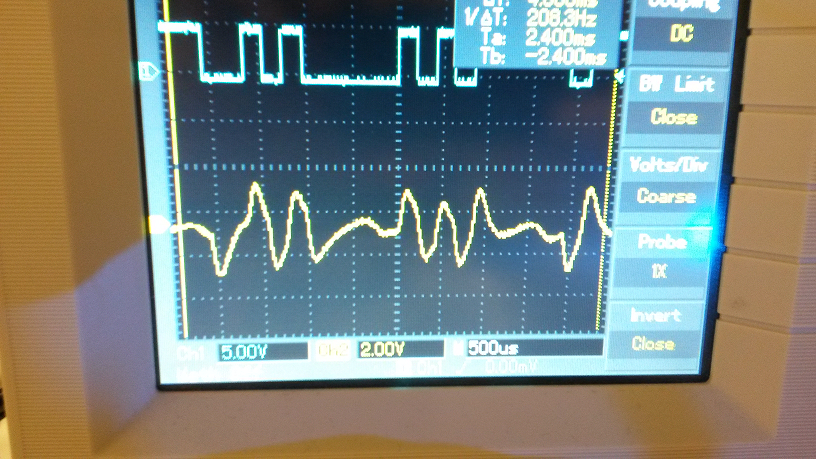
\includegraphics[width=0.8\textwidth]{pic1}
\caption{Filter paramter variation 1  and reconstructed signal}
\label{fig:rec}
\end{figure}

\begin{figure}[h]
\centering
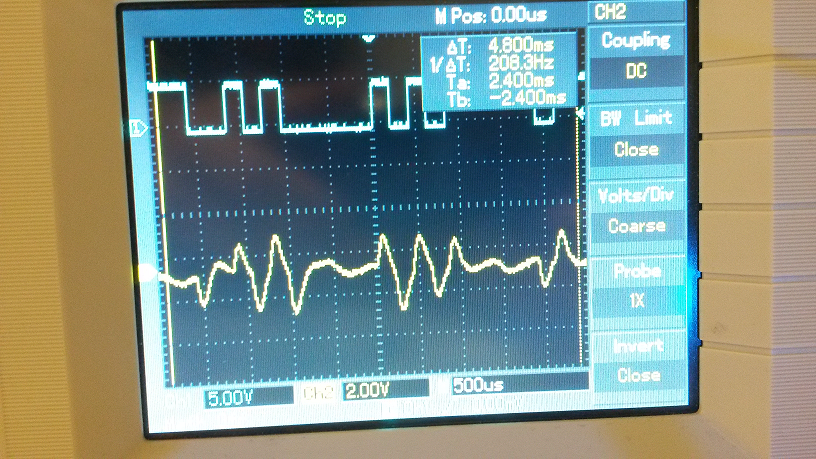
\includegraphics[width=0.8\textwidth]{pic2}
\caption{Filter paramter variation 2 and reconstructed signal}
\label{fig:rec}
\end{figure}




\subsection{Communication part (Sudhangathan Bankarusamy)}

\subsubsection{The prototype}
This setup consists of an LED and photodiode, each of them connected to a Beagle Bone Black(BBB). The LED and photodiode electronic circuits are explained in the electronics section. Figure~\ref{fig:vlc_proto} shows the actual setup. In this prototype version the OpenVLC framework is not used for the lack of time. Instead a simplex serial communication is emulated using light over air.
\begin{figure}
\centering
        \includegraphics[totalheight=8cm]{prototype_VLC.eps}
    \caption{Prototype: Picture of the lab setup}
    \label{fig:vlc_proto}
\end{figure}



\subsubsection{Transmission and receiving of information}
The bits of information is sent to the LED over the serial port, TX, of the BBB. While on the receiving side a photodiode is connected to the RX of the BBB. Any application that uses serial port to transmit information can be used with such a setup. In this case, minicom was used to send and receive characters. Both the BBBs were connected to a laptop. Two different serial terminals were used to connect to both the BBBs and the character send/receive experiment is done. \\
Table~\ref{tab:setupinfo} shows the setup parameters.
\begin{table}[h]
\centering
\caption{Prototype parameters}
\label{tab:setupinfo}
\begin{tabular}{|c|c|}
\hline \textbf{Parameter} & \textbf{Value} \\ 
\hline Baud rate achieved(stable) & 2400 bps \\ 
\hline Distance (stable) & 1.6 m \\
\hline LED power & 1 W \\ 
\hline Wave length & 473nm(Blue) \\ 
\hline Rx pin number(RX BBB) & P9:23 (UART1\_RXD) \\ 
\hline Tx pin number(TX BBB) & P9:24 (UART1\_TXD) \\ 
\hline 
\end{tabular} 
\end{table}



\subsection{Conclusion(Albin Barklund)}
The method works and the technology could probably be used for under water communication even tough it is most likely not a good solution. This is due to the fact arbitrary digital signals contain many different frequencies and the modulation scheme suggests sending all of them through the medium.

\subsection{Future work}
A better approach would be to implement a data link with LEDs and photodiodes which uses a FSK modulation scheme instead.





















\section{Sonar communication(Peter Cederblad)}
\label{sec:Sonarcommunication}

\subsection{Introduction}
In order for the underwater robots to be able to communicate for long distances, a sonar communication system needs to be implemented.
Only a basic prestudie has taken place in this subject during this fall. It has been decided that this shall be Albin Barklund and Daniel Adolfssons master thesis work.




\section{Swarm behavior}
\label{sec:Swarmbehavior}

\subsection{Intoduction (Peter Cederblad)}
In this part of the project there has been an investigation in collaboration between robots. Especially how to form shapes. This will be useful for the e.g. the schools underwater robots that will search and mark oil leakage. 

The first thing any robot collective needs is a coordinate system, that has been the first of two things that this year has focused on. The second thing is to make a good starting point for the next year in terms of producing startup code for the kilobots, in c and to create a simulation environment in Matlab



\subsection{Kilobot code}
For a land based platform the kilobot platform~\cite{kilobotsK-Team} was chosen after a few weeks of investigation on different platforms. For the kilobots there has been produced a number of small programs for the students to start with, in order for them to get a quick introduction on how the kilobot API works~\cite{kilobotsK-Team}. These small programs consist of finished exercises. Exercises that was written for a different library~\cite{kilobotsLabs}, than the one that followed with the kilobots when they were purchased.\\
A short description will be included her for each program.
\begin{itemize}
\item \textbf{Lab0\_Blinky.c}\\
This is the first program to start with. It introduces a basic function and the purpose of this program is to show how to manipulate the onboard LED.
Functions used are: Robot\_ID(), set\_color(), \_delay\_ms() and also in the main function init\_robot() and main\_program\_loop().\\
The main function is the same in all programs and should never be changed, except with which function name the main\_program\_loop() should call.

\item \textbf{Lab1\_1\_Simple\_movment.c}\\
In this program the motors are added. They use two different function.\\
spinup\_motors() and set\_motor(). Here the robot will move forward for a while and then turn in both directions. The robot will also turn on the LED in different colors.

\item \textbf{Lab1\_2\_Nonblocking\_movment.c}\\
The non-blocking program does the same thing as the first program, except this one take uses interrupt routines.

\item \textbf{Lab2\_1\_Test\_speaker.c}\\
Here the communication begins. The function message\_out() is introduced now and the variable enable\_tx. Which tells the robot that it is allowed to transmit messages. The robot will broadcast a fixed message.
Program one robot with this program and another as a listener. 

\item \textbf{Lab2\_2\_Test\_listener.c}\\
This is the second part in the communication. The receiving robot. The get\_message() function is used to collect messages and put it in the message\_rx array. The program will also blink when a message is received.

\item \textbf{LAB2\_3\_Test\_speaker\_mod.c}\\
Now timeing is added. This program uses the variable kilo\_ticks which can be located in the libkilobot.c file, inorder to keep track off the time. It will then transmit a 0 or a 1 every other time. And off course blink in different colors depending if it is a 0 or a 1 in the message.

\item \textbf{Lab2\_4\_Test\_listener\_mod.c}\\
The message array is further explored in this program. First the robot looks if the number is even or odd, it the reads the distance from the sending robot. The LED is turn on and off in different colors depending on those to factors.

\item \textbf{Lab3\_Putting\_it\_together.c}\\
A multitasking robot is created here. It both sends and reads messages. If the robot receives a message it will start its motors in a random direction. This will make all robots, with time, lose connection to all there friends. When the robot does not receive any new messages it will stop and turn the LED white.

\item \textbf{Lab4\_1\_Orbit\_star.c}\\%Here it is required to have two robots.
This exercise requires two robots. One that can reuse the code from\\
 Lab2\_1\_Test\_speaker.c, this robot will akt as a star. The other robot will receive messages from the star and it will try to move around the star in a circle with a fixed distance. This program in it self does not provide any real new functionality, but it is a good program to build more of. Add more robots and make them all move around the same star without crashing into one another.

\item \textbf{Lab5\_Move\_to\_light.c}\\
The kilobots also has an ambient light sensor. In this program the robots will try to move towards the light. This requires a dark space.
four new function is used here. Mean\_Ambient\_Light(), kprinti(), kprints() and abs().

\item \textbf{Lab6\_2\_Gradient\_simple.c}\\
This program is the first one that can be called a little more advanced. Here the robots calculate distance in form of information hops from one predefined seed robot. Each robot will indicate the distance by turning on different colors on the LED.

\item \textbf{Lab6\_Gradient\_adptive.c}\\
This program is similar to the above, but here a timer is implemented as the gradient can change with time.

\item \textbf{Lab7\_sync.c}\\
In the sync program all robots start up with a random delay, and then makes a blink in a specific period, they also sends out a message so the neighbors know when the robot blinks. All robots will then change a little bit on the period of blinking in order to try to match up with each other. With time they will start to blink in sync.
\end{itemize}

There has also been created a .c file whith some start up code and the structure for the S-DASH. It is called SelfAssemblySelfHealing.c\\
Functions that has been added to the predefined libkilobot.c are the following.\\
The four first are more general for the kilobots, while the purpose of the rest is for the S-DASH algorithm:
\begin{itemize}
\item \textbf{extern int RobotID(int modulusWith)}\\
This function collects sensor data from the ambient light sensor. It will then use this data to create a random number, which will be modulated with the input integer value. The function returns an integer value.

\item \textbf{extern void spinup\_motors(int num)}\\
For the kilobots to be able to move, they have to overcome the static friction between the legs and the surface. This function does just that. It will set the motor/motors on maximum value for 10ms. After this function the SetMotion() function shall be called. The input is an integer corresponding to which motor to turn on or both.
\begin{itemize}
\item 1: Both motors, this will make the robot ready to move the forward direction.
\item 2: Right motor, this will make the robot ready to rotate in a counterclockwise direction.
\item 3: Left motor, this will make the robot ready to rotate in a clockwise direction.
\end{itemize}

\item \textbf{extern void SetMotion(int current\_motion, int Direction)}\\
This is the second function that has to be called in order to make the kilobots to move. It works in a similar way as spinup\_motors(), but the motor values are lower. The four global variables cw\_in\_straight, ccw\_in\_straight, cw\_in\_place and ccw\_in\_place are used. These variables can be tuned in order to make each kilobot move the desired bahavior.

\item \textbf{extern int Mean\_Ambient\_Light(int num)}\\
This function takes in an integer value. This integer is the amount of samples that shall be collected from the ambient light sensor. The function returns the mean value of all samples.

\item \textbf{extern int fakultet(int N)}\\
Calculates the factorial of the input integer and returns that number.

\item \textbf{extern void SwapChar(char* str,int i, int j)}\\
Change place on two characters in one array

\item \textbf{extern void SwapInt(int arr[],int i, int j)}\\
Change place on two integers in one array.

\item \textbf{extern void PermuteStr(char* Ans, char* string, int start, int end)}\\
The purpose of this function is to calculate all combinations of neighbors when checking which neighbors that can for a referensgrupp for the triangulation as well as for merging groups in the S-DASH algorithm.\\
It takes in an string and prints out all combinations on the computer screen using the kprints() function.\\
This function can be changed inorder to store the values for the robot to use instead of printing them on the screen

\item \textbf{extern void PermuteInt(int Ans, int array[], int start, int end)}\\
This function does the same thing as the above, but with and array of integers.The reason for the two implementations, is because the students for the up coming year can choose how to represent the neighbors.

\item \textbf{extern void CheckAllNeighborsID(int neighbor\_ID[], int neighbor\_Dist[])}\\
This function takes in an robot id value and the distance fromthat robot, it then
\end{itemize}
All the above functions can be found at the bottom inside the libkilobot.c file.



\subsection{Matlab code}
In this project Matlab 2015b has been used.
There has been 3 major .m programs produced in this project. 
\begin{itemize}
\item $NetWorkControlSystems\_test.m$:This file shows how to solve some basic problems in swarm robotics; Solving the rendezvous problem is one of them. Also how to form basic constellations and make that constellation change direction, move around in a user input way and also follow a predefined path. This file is mostly for getting into swarm thinking, using ordinary vector programming in Matlab. Here only Matlab's own coordinate system is used.

\item $ClassTest.m$: Here we take the next step and start looking at objectoriented programming with Matlab. This program solves a little more comlicated problems. First all agents are wandering around randomly untill they see some one else. When this happens they calculate the rendezvous point between all agents that see each other at that area. If there are several small groups created in the Matlab world, they do not take each other into account in this calculation. When a group of agents are close enough to each other they will start to wander in some predefined direction. Here there are room for future work. They should continue to search the environment for more agents. Three different end conditions could be implemented.
\begin{itemize}
\item The maximum number of agents are known and the seach continues untill all all agents belong in one consistens group.

\item A search time counts down and resets for every new agents that are found, when search timer reaches zero. All search groups defines the world population as there own group. They can after this start to solve what ever task the human has given to them.
\item Same as number two, but with an extra deadline that can not be reset. This would mean that the maximum time that the agents has can not be broken, this resembles a search and rescue setup.
\end{itemize}

\item $SelfOrganizingCoordinateSystemTest3\_6.m$: This is the most advanced .m file and it is crucial for the swarm behavior part of this project that it is finished. The purpose with this program is to construct a consistent coordinate system between all agents that can communicate with each other and measure distances. This is not fully implemented in a robust way. It is possible to get a consistent coordinate system in some special cases, but more work has to be done here.\\
The purpose to have a local coordinate system that all agents can agree upon, is that it will be easier to solve tasks together if every one in the group knows were they are all the time, without the use of external coordinate systems as GPS.\\
This self-organizing coordinate system is the first part of the S-DASH algorithm.
\end{itemize}









\subsection{S-DASH }
This will be a short deskripten of the scalable - distributed self-assembly and self-healing algorithm (S-DASH), for more detaljs see \cite{Ruben}.\\
The S-DASH consists of four main parts.\\
\begin{itemize}
\item First it develops a \textbf{consistent coordinate system} that all agents can agree up on. First a set of at least two seed agents must be chosen and then these seed agents will choose two more reference robots. The second part is to use trilateration, which in geometry is a way to determine relative and absolute points when the agents can measure distances. Now there will be at least two local coordinate systems, one for every seed agent. Next step is to merge all local coordinate systems and create a transitional coordinate system that all agents in the collective can relate to. This is implemented in the $SelfOrganizingCoordinateSystemTest3\_6.m$ file and all steps in this test file is well commented. How ever the simulation file needs to be reviewed, it does not have a robust behavior in the end for agents that do not sit in Matlab's orion.

\item The second part is \textbf{DASH}, the inputs for this function are the desired shape of the collective, given as a picture or a pixel map(black and white, white pixels belong to the shape), desired scale of the shape, robot location in the self-organized coordinate system and messages from neighbors. It will then use the gradient map to decide how to move. It chooses what to do after calculating:
\begin{equation}
\theta_{gradient} = atan\frac{A}{B}
\end{equation}
Where gm is the gradient map and\\
$A = gm(x_{index}, y_{index}+1) - gm(x_{index}, y_{index}-1)$\\
$B =  gm(x_{index}+1, y_{index}) - gm(x_{index}-1, y_{index})$\\

Then it has five modes: Gradient follow, trapped robot message, trapped robot moment, random moment and stop movement.
Each pixel in the pixel map can be indexed by two numbers$(x,y)$, where y represent how many pixels there are above current pixel and x represent how many pixels that are to the left of this pixel.
This will give the upper left corner$ (x,y) = (0,0)$.
There are two constraints here.
\begin{itemize}
\item connected shape.
\item All pixels on the outside border must be black.
\end{itemize}

Next we have the scale, $S_f$, defines in terms of robot radius, $R_{robot}$.
IF the shape is a  square $3x3$ pixels. AND $S_f = 2.0$
THEN each pixel will be $2*R_{robot}$ wide and  $2*R_{robot} $long, this means that the dimensions of the real shape will be  $6*R_{robot}$ wide and  $6*R_{robot}$ long.

\item The third part is to determine the \textbf{scale} of the scape that is proportional to the number of agents currently in the collective.

Every time step every robot updates it’s  $S_f $to the mean of it’s own and all neighbors. 
After this the robot communicates this to all it’s neighbors.
IF the scale is too big then all robots has to reduce there scale. This is done in three steps.
\begin{itemize}
\item A distributed mechanism to let all robots know that the seed position is unoccupied.
\item A way to know how long time to wait until the seed position should have been taken.
\item A mechanism to reduce the scale.
\end{itemize}


\textbf{Detecting unoccupied seed:}
$T_{unoccupied}$ updates as following. $T_{unoccupied}$ is compared with all neighbors $T_{unoccupied}$.
IF there are any neighbors value that is lower then its own value of $T_{unoccupied}$ THEN $T_{unoccupied} = neighbors value + 1$.
IF no neighbors value are lower THEN increase own value with 1.
IF the robot is located in the seed position THEN set $T_{unoccupied}$ value to zero and update all neighbors.

Above pseudoAlgo will have the effect as a timer. If no robot is located at the seed position, then all robots will start to increase there $T_{unoccupied}$ value by one for every loop in the main controller.
Eventually one robot will reach $T_{unoccupied_{max}}$ which will tell the robot that the scale is to big.

The $T_{unoccupied_{max}}$ is calculated as followed.
\begin{equation}
T_{unoccupied_{max}} = \frac{S_{f} * L_{externalpath}} {V_{robot}*P_{move}}
\end{equation}
This means: The worst case of traveling  divided with the average moment speed.
where,\\
$S_f	= Current scale factor$\\
$L_{external_path} =$\\ Max(The distance between the starting pixel outside the shape and all pixels on the border of the shape)\\
$V_{robot} =$ Speed of the robot movement\\
$P_{move}	 =$ The probability that the robot will move

\textbf{Reducing the scale:}
The scale reduction is initiated by the first robot to reach $T_{unoccupied_{max}}$ or go above it. NOW this robot will do two things:
\begin{itemize}
\item Set it’s own $T_{unoccupied}$ value to 0
\item For $\frac{T_{unoccupied_{max}}}{2}$ cycles of the main control loop, do not use the ordinary scale update function, instead report to all neighbors the new lower value $S_{f_{new}}$. This will effect all robots $S_f$ value.

The $S_{f_{new}}$ is calculated as following:
\begin{equation}
S_{f_{new}} = S_{f_{old}} * sqrt(1-(\frac{1}{NumPix}))
\end{equation}
where NumPix is the total number of pixels in the shape pixel map’s shape segment.
\end{itemize}

However after that the scale has been observed for a long time and it is not big enough, three things needs to take place, similar as when the scale is to big.
\begin{itemize}
\item A distributed mechanism to let all robots know that the external segment seed position is occupied.
\item A way to now how long time to wait until the seed position should have be free.
\item A mechanism to increase the scale a proper amount.
\end{itemize}

\textbf{Detecting occupied seed:}
$T_{Occupied}$ this variable is updated every loop in the main controller, just as $T_{unoccupied}$. In every cycle the robot checks to see if it is in the external segments seed position. IF true, then $T_{Occupied} = T_{Occupied} +1$.
IF the robot receives a message called ”$moved\_into\_shape\_message$” then it will put a zero in the $T_{Occupied}$ variable. IF $T_{Occupied}  < T_{Occupied_{max}}$ then it is time to increase the scale.
The robot will also send out the $moved\_into\_shape\_message$.
	
\textbf{Wait time:}
The definition for $T_{Occupied_{max}}$ is the same as the definition of $T_{unoccupied_{max}}$ except for the $L_{internalpath}$,
which is defined as: Max(The distance between the starting pixel inside the shape and all pixels on the border of the shape)

\textbf{Increasing the scale:}
The robot that initiate the increase scale do two things:
\begin{itemize}
\item Send out the $moved\_into\_shape\_message$, to prevent other robots from further trying to increase the scale by resetting the $T_{Occupied}$ values.
\item For $\frac{T_{Occupied}}{2}$ cycles of their main controller loop, they do not use the original update function(same as above) instead they send out a new larger scale value  $S_{f_{new}}$.
$S_{f_{new}} = sqrt(S_{f_{old}}^2 + (Pi/NumPix))$.
\end{itemize}

\item The last and fourth part is to \textbf{choose a role} based on its location within the shape and with respect to time(partial-temporal differention)
This is a distributed method to allow each robot to choose a role based on its location in the desired shape and time.
The overall choice of all robots in the shape is called the partial-temporal role pattern. This pattern is given to each and every robot in the form of a pixel map or an image, called the partial-temporal role map.
Inputs for this function are the spartial-temporal role map(or just a Spartal role map), desired scale and the robots location in the coordinate system. 
The function shall do the folowing: All robots has either an Spartal role map(1) or Spartal-temporal role map(2).
IF(1) THEN each entity in the map consists of just an integer value, which represents a role.
\begin{table}[h]
\caption{The spartial role map} \label{tab:numbersExample}
\begin{center}
\begin{tabular}{| l | l | l | l |}
\hline
1 & 1 & 1 & 1 \\ \hline
1 & 2 & 2 & 1 \\ \hline
1 & 2 & 2 & 1 \\ \hline
1 & 1 & 1 & 1 \\ \hline
\end{tabular}
\end{center}
\end{table}

In the above example  there are to different roles, ”1” and ”2”. The outer part has role number ”1” and the inner robots will have role ”2”. This could represent different colors on the leds or other things.\\
IF(2) THEN each entity in the map consist of a list of paired numbers. A timestamp and a role.
\begin{table}[h]
\caption{The spartial-temporal role map} \label{tab:numbersExample}
\begin{center}
\begin{tabular}{| l | l | l | l |}
\hline
(0,1) & (0,1) & (0,2) & (0,2) \\ 
(1,1) & (1,1) & (1,1) & (1,1) \\ \hline
(0,1) & (0,1) & (0,2) & (0,2) \\ 
(1,2) & (1,2) & (1,2) & (1,2) \\ \hline
(0,1) & (0,1) & (0,2) & (0,2) \\ 
(1,1) & (1,1) & (1,1) & (1,1) \\ \hline
(0,1) & (0,1) & (0,2) & (0,2) \\ 
(1,2) & (1,2) & (1,2) & (1,2) \\ \hline
\end{tabular}
\end{center}
\end{table}

\end{itemize}


In the above example: At time = 0, The robots in the left halv of the square should choose role ”1”  and the robots on the right side will take on role ”2”. This will be the first () in each entity. The second () in each entity corresponds to the second timestep. 





\subsection{Conclusions}
The simulation environment for the self-organizing coordinate system took far more time to develop then expected.
Things to note about the experimental design is that the test cases shall not just be to small which is common knowledge, but also the minimum size of the testcases had an hugh impact.
\subsection{Future work}
Finish the implementation of the S-DASH algorithm, both in Matlab and in c code.


\newpage


\newpage
\section{Appendices}
\appendix
\label{App:appendix}
\section{IMU - Bomlist(Roxanne Anderberg)} \label{App:IMUBomlist}
\begin{table}[ht]
	\centering
	\resizebox{\linewidth}{!}{%
	\begin{tabular}{|l|l|l|l|l|l|}
    \hline
  \multicolumn{6}{|c|}{BOM} \\
  \hline
	Name & Vendor & Ordernr & RefDes & Value & Shape \\ \hline
	Electrolyte Capacitor & Würth & 865230640001 & C1 & 0.1uF & CAPAE430X540N \\ \hline
	Electrolyte Capacitor & Würth & 865230640001 & C2 & 0.1uF & CAPAE430X540N \\ \hline
	Electrolyte Capacitor & Würth & 865230640001 & C3 & 0.1uF & CAPAE430X540N \\ \hline
	Electrolyte Capacitor & Würth & 865230640001 & C25 & 0.1uF & CAPAE430X540N \\ \hline
	Harwin male connector & Farnell & 1144561 & IMU\_CON & HDR2X5 & Harwin\_Male \\ \hline
	LED SMD & School &  & LED4 & LED\_blue & INDC1608X95N \\ \hline
	2.54 mm pin header & Würth & 61300411121 & POWER & HDR1X4 & HDR1X4 \\ \hline
	Resistor SMD & School &  & R24 & 2.2kOhm & RESC1608X63N \\ \hline
	2.54 mm socket head & Würth & 61300211821 & TEST\_HEADER & HDR1X2 & HDR1X2 \\ \hline	
	2.54 mm socket head & Würth & 61300211821 & TEST\_JP & HDR1X2 & HDR1X2 \\ \hline
	Tranceiver & Farnell & 9724370 & U12 & MAX232AEWE+ & SOIC127P1032X265-16N \\ \hline	
	2.54 mm pin header & Würth & 61300411121 & UART1 & HDR1X4 & HDR1X4 \\ \hline
	2.54 mm pin header & Würth & 61300411121 & UART2 & HDR1X4 & HDR1X4 \\ \hline
	\end{tabular}}
	\newline
	\caption{BOM} \label{BOM}
\end{table}


%\vspace{20 mm}



\section{IMU - Schematics and CAD} \label{App:IMUSchematicsAndCAD}
The schematics have made in multisim and the CAD files have been made in ultiboard.


\begin{figure}[!htbp]
    \centering
        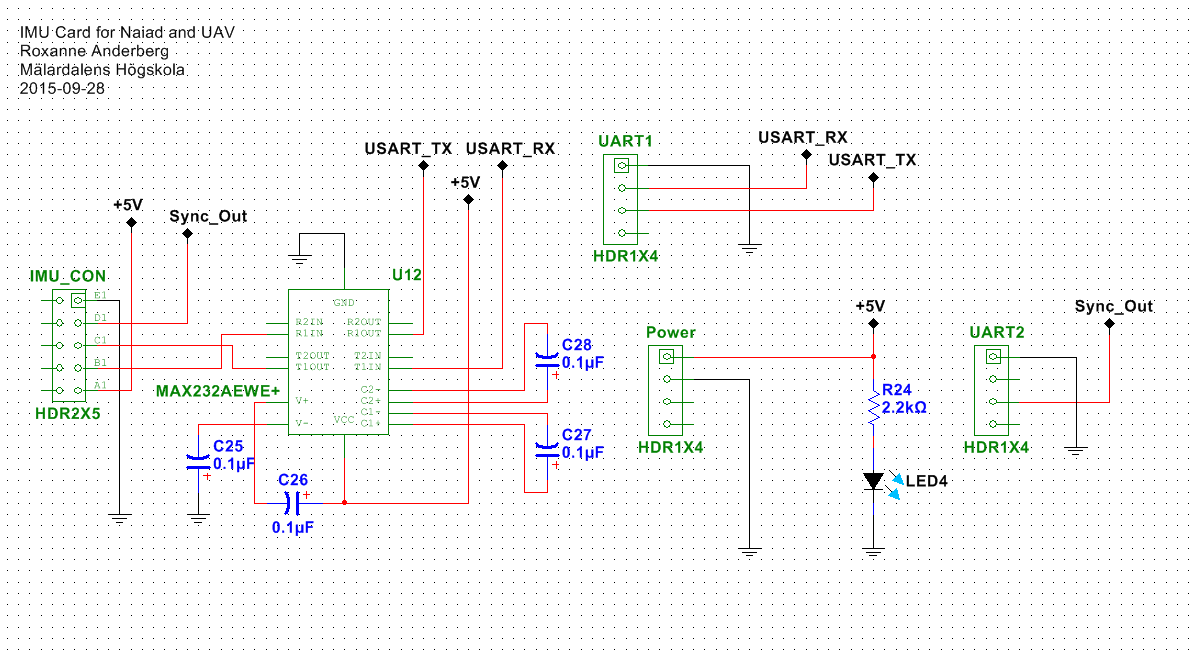
\includegraphics[width = \columnwidth]{IMUschematics}
        \caption{Schematics for the UART RS-232 adapter} \label{schematics}
\end{figure}


\begin{figure}[!htbp]
\centering
    %\begin{subfigure}[b]{\textwidth}     
    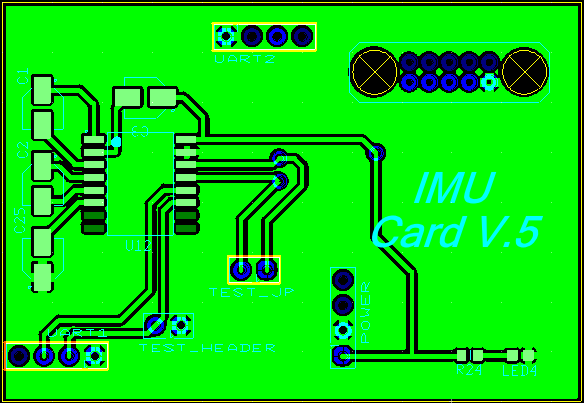
\includegraphics[scale=0.5]{IMUcoppertop}
        \caption{Top Layer}
        \label{fig:top}
  %  \end{subfigure}
    
    ~ %add desired spacing between images, e. g. ~, \quad, \qquad, \hfill etc. 
      %(or a blank line to force the subfigure onto a new line)
  %  \begin{subfigure}[b]{\textwidth}
        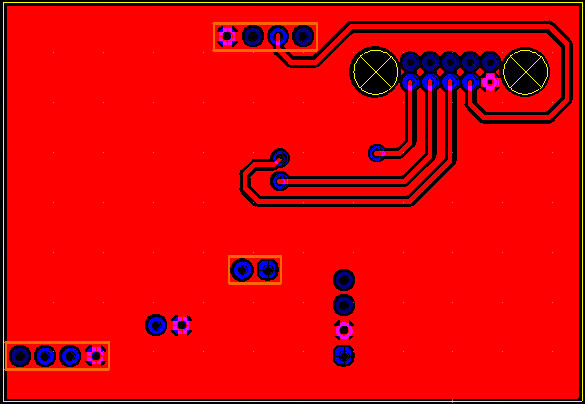
\includegraphics[scale=0.7]{IMUcopperbottom}
        \caption{Bottom Layer}
        \label{fig:bottom}
  %  \end{subfigure}
    \caption{CAD model of the extension card}\label{fig:CADmodel}
\end{figure}




\newpage
\section{Mechanics Group's report(Ragnar Moberg)} \label{App:MechanicsReport}
\begin{figure}[!htbp]
\centering  
    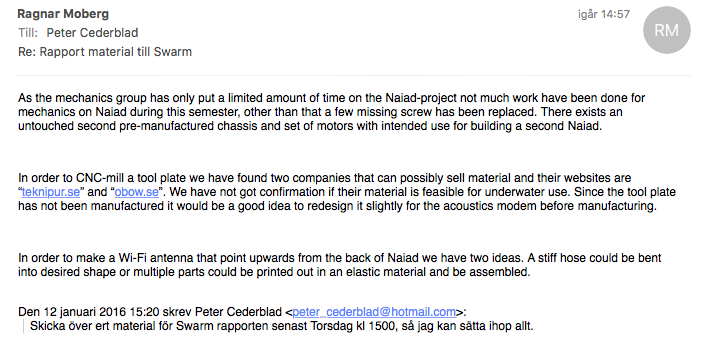
\includegraphics[scale=0.7]{Mechanics_Report}
        %\caption{Mechanics Group's report}
        \label{fig:M_R}
\end{figure}





\newpage
\section{Light communication - BOM(Albin Barklund)}\label{App:LightCommunicationBOM}
\begin{tabular}{l l l}
{\bf Name} & {\bf Vendor} & {\bf Ordernumber}\\
Blue LED & DigiKey & XPCBLU-L1-R250-00V01TR-ND \\
Photodiode Blue & DigiKey & SD019-141-411-BCT-ND\\
\end{tabular}


\section{Trello Cards(Peter Cederblad)}
\subsection{Comunication trello Cards}


  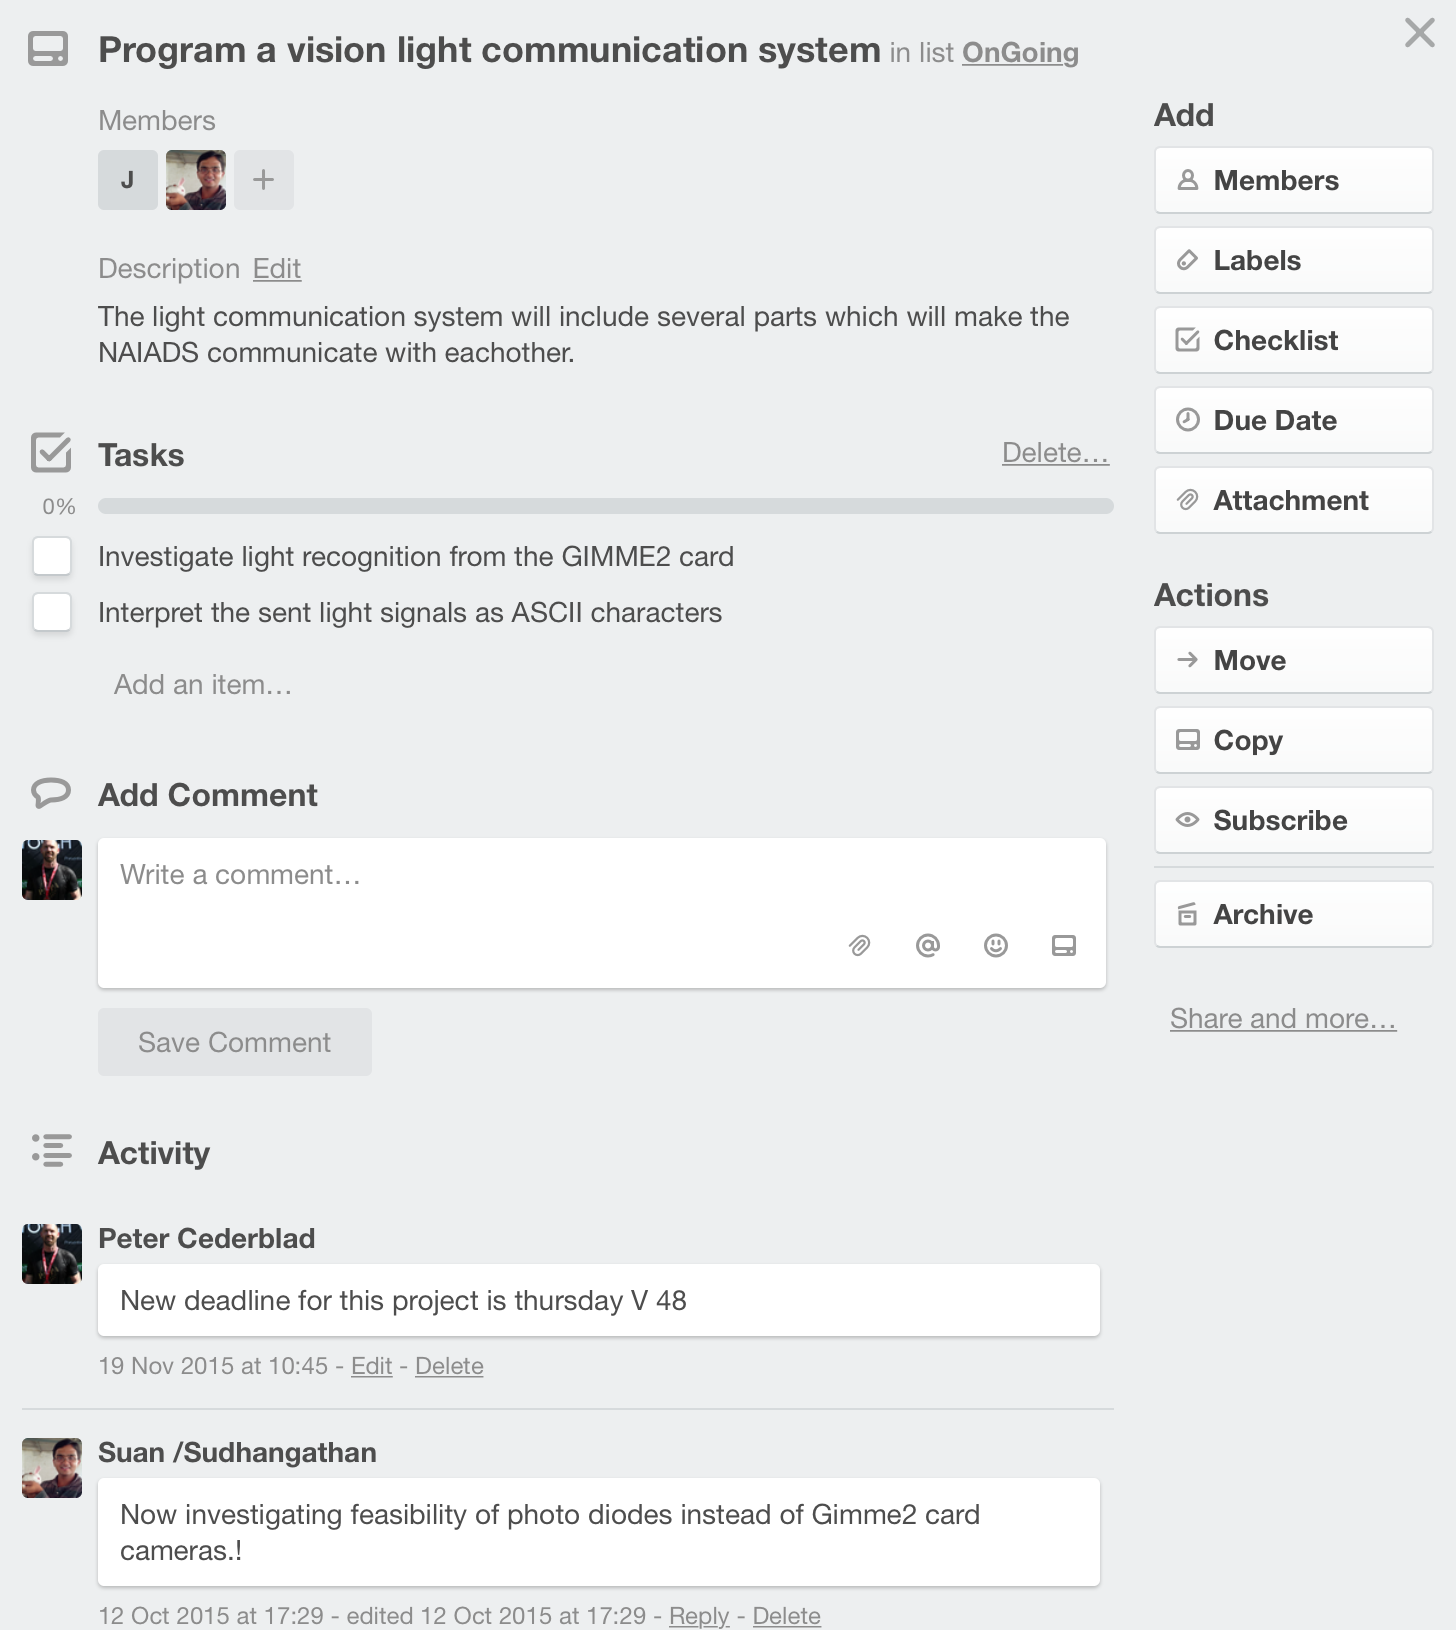
\includegraphics[scale=0.5]{Screenshoot1}

  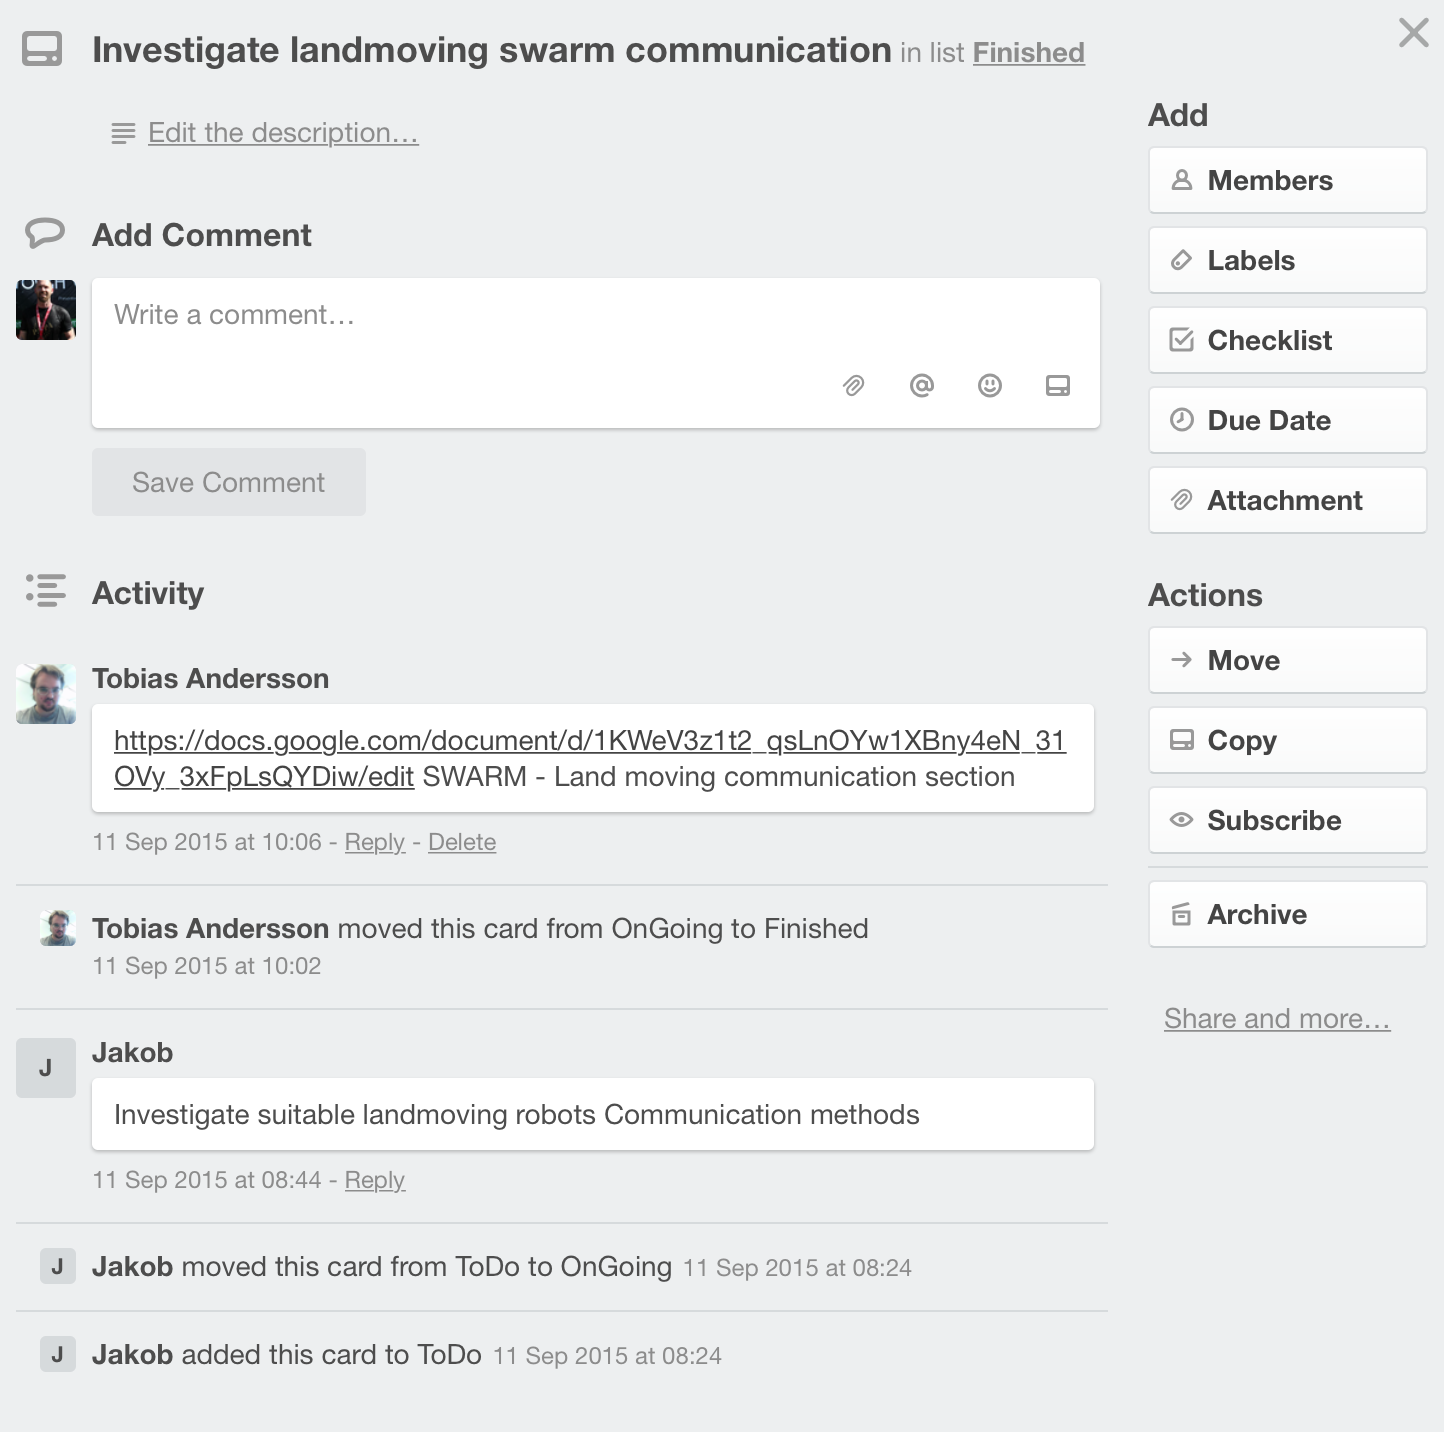
\includegraphics[scale=0.5]{Screenshoot2}
\newpage
  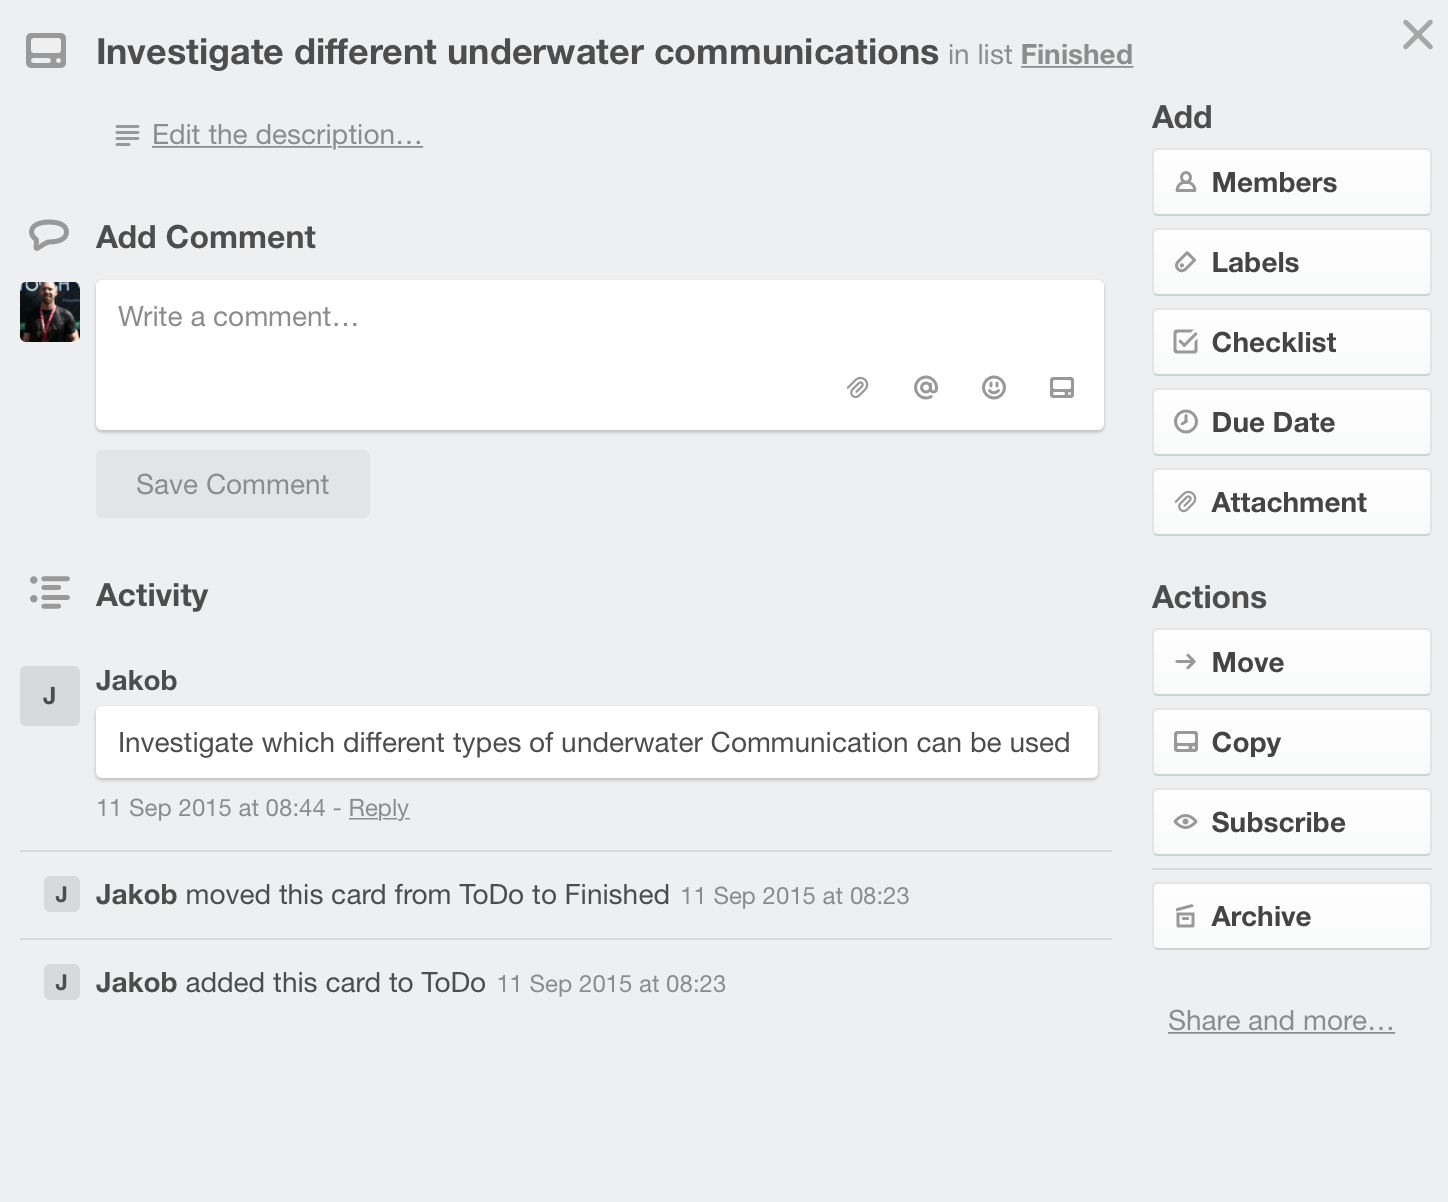
\includegraphics[scale=0.5]{Screenshoot3}

  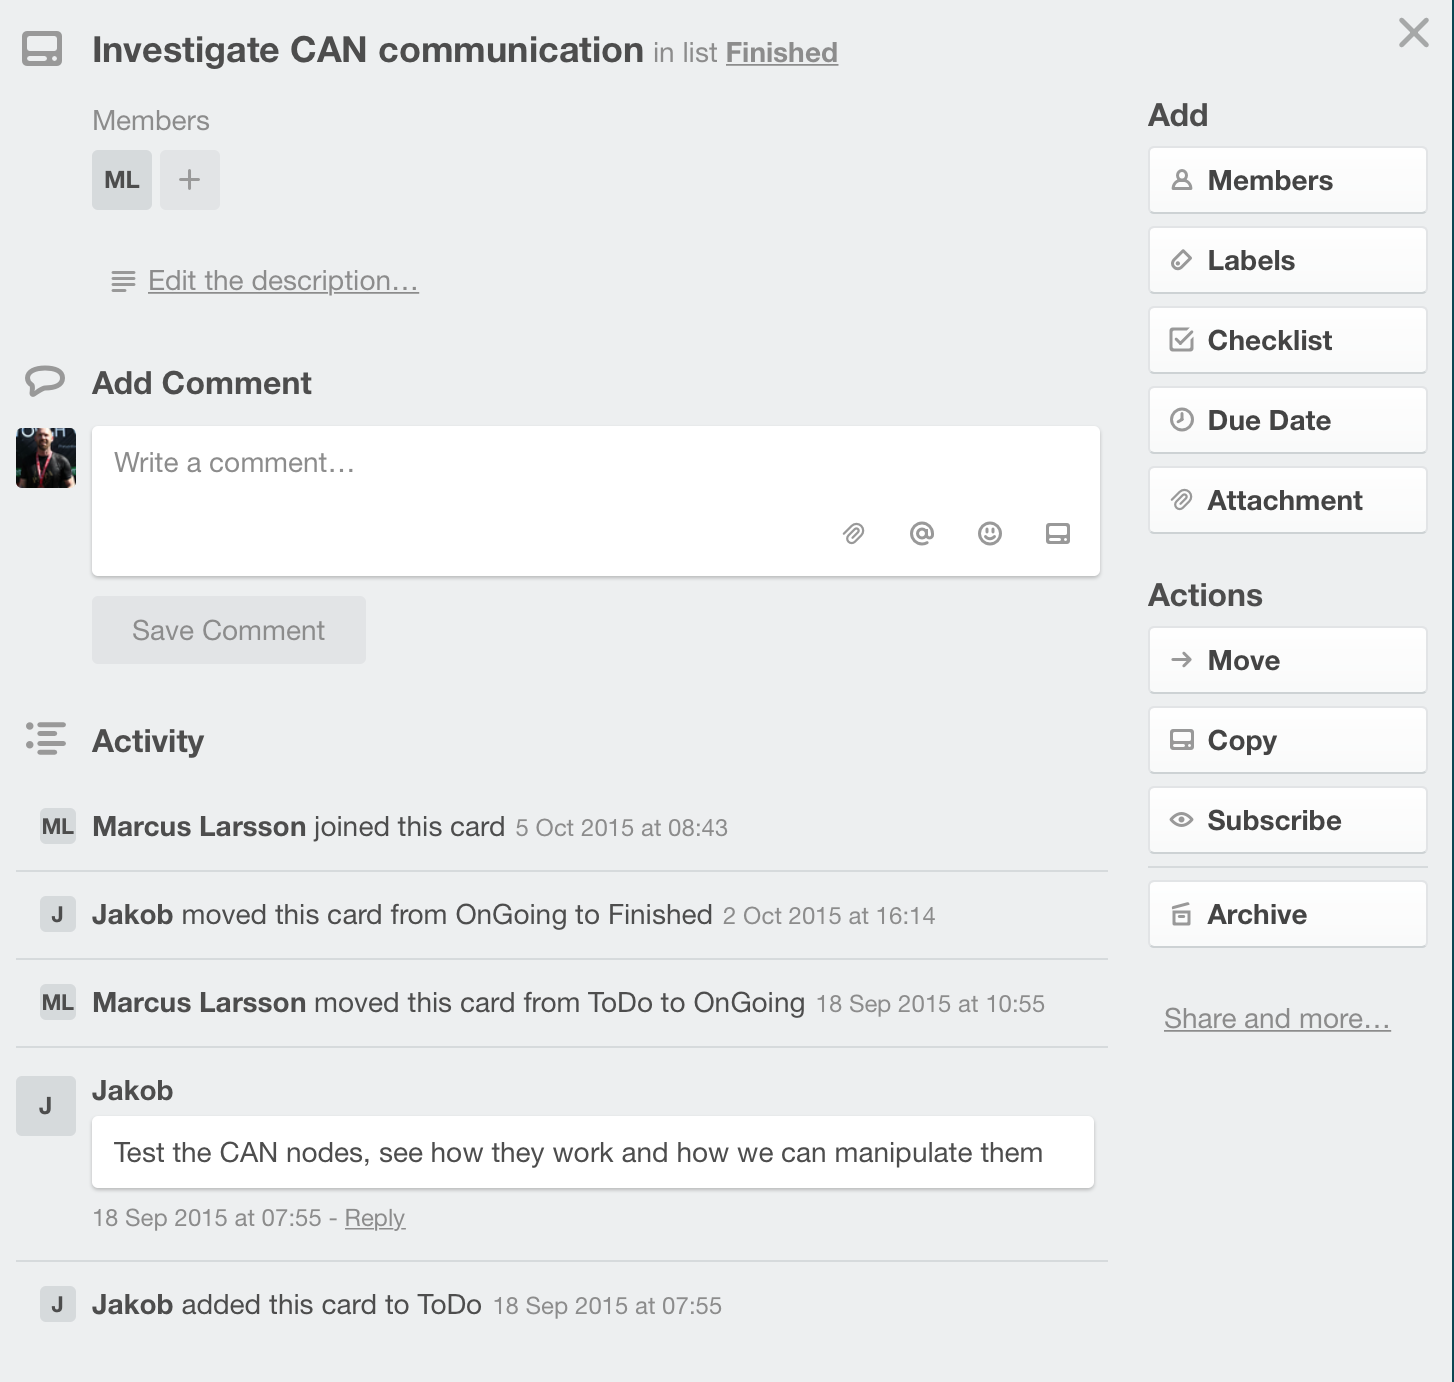
\includegraphics[scale=0.5]{Screenshoot4}


\newpage
\subsection{Hardware trello Cards}

    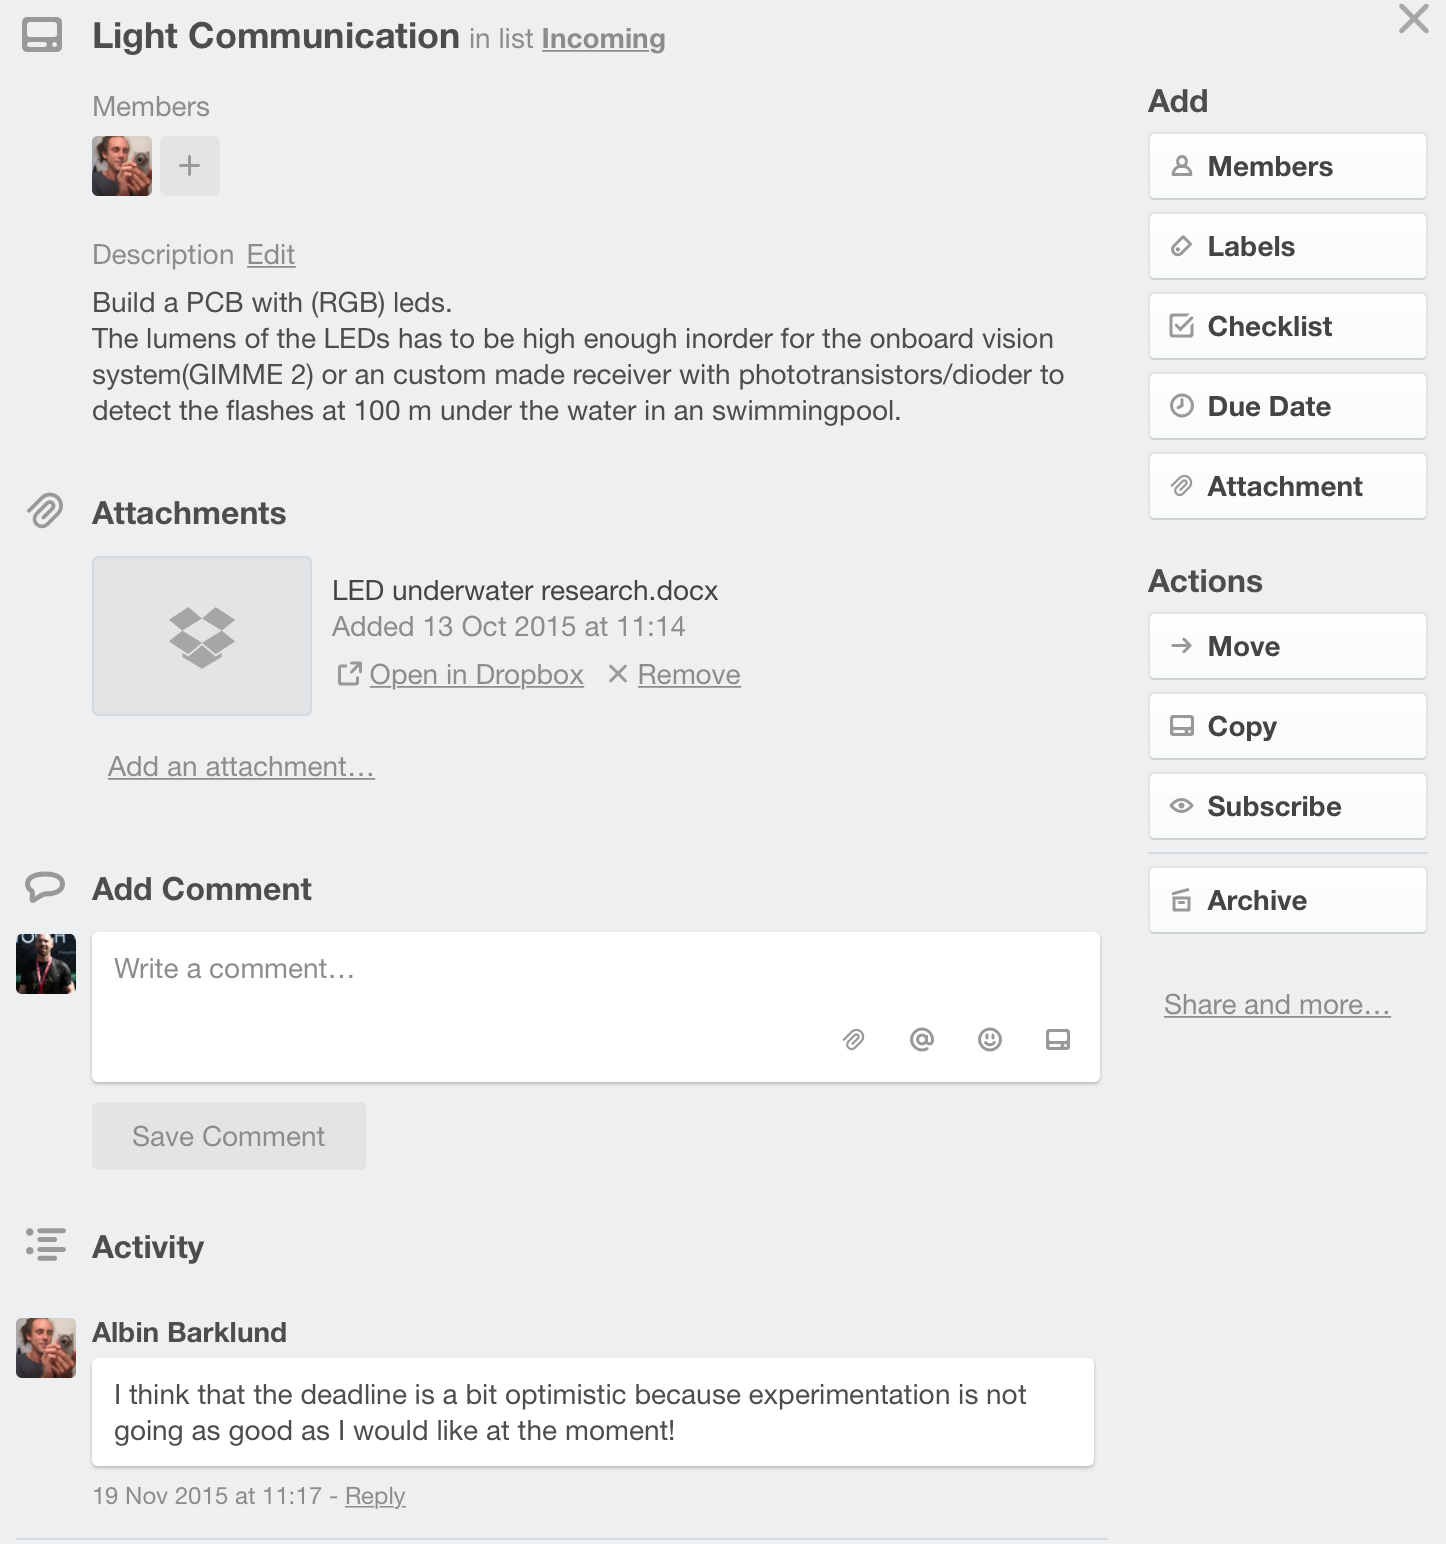
\includegraphics[scale=0.5]{Screenshoot5}



    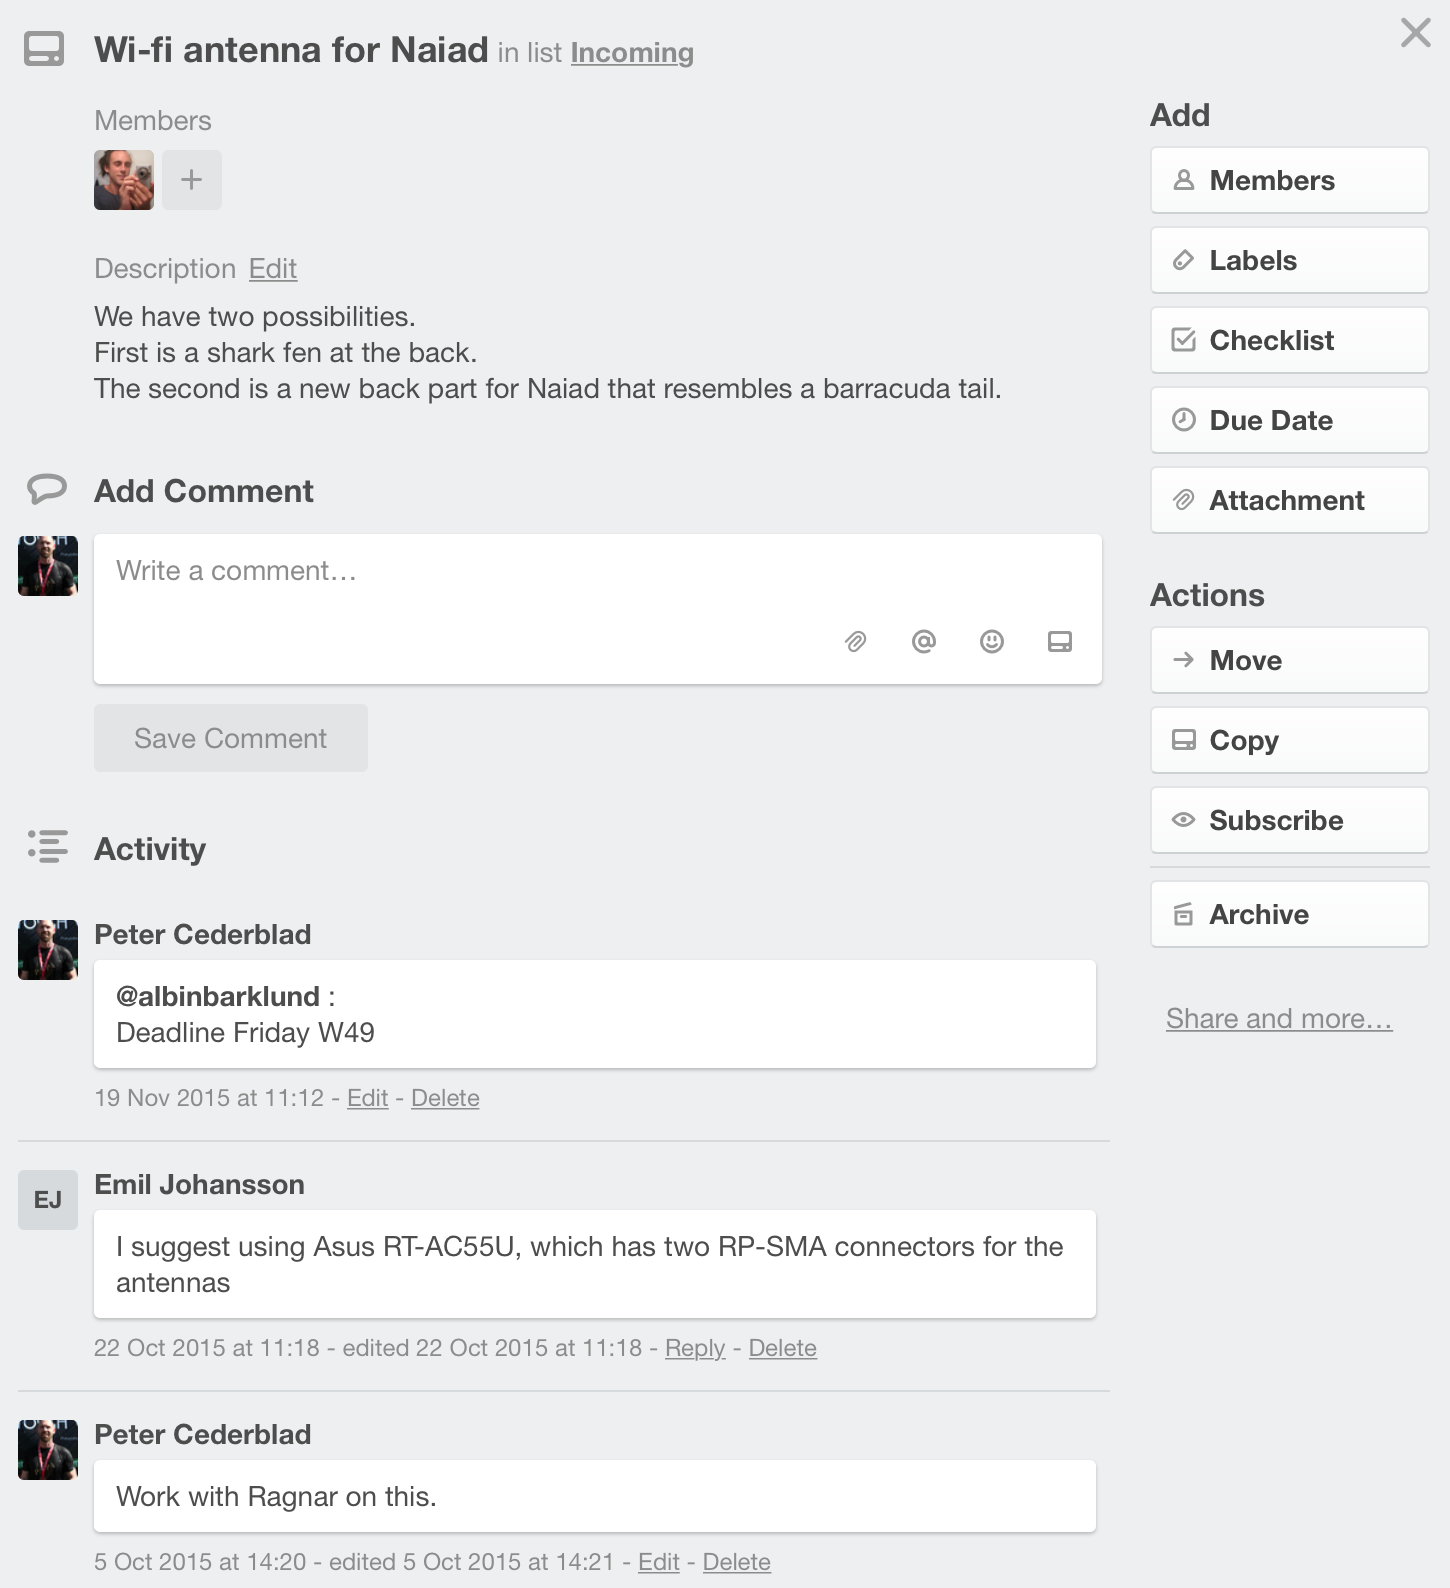
\includegraphics[scale=0.5]{Screenshoot6}



    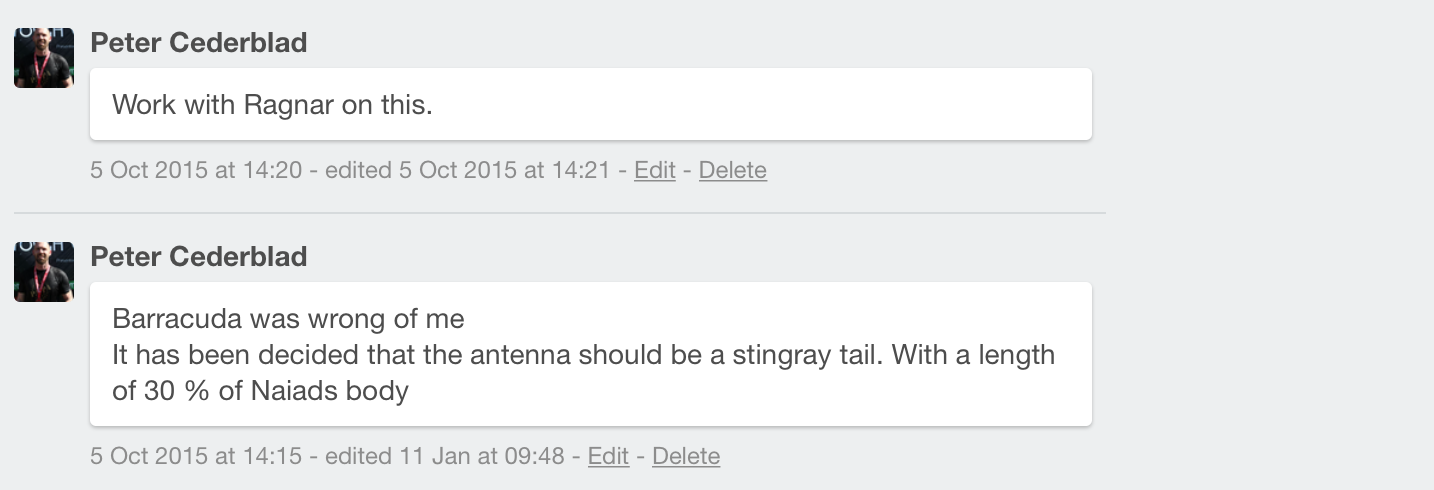
\includegraphics[scale=0.5]{Screenshoot7}




    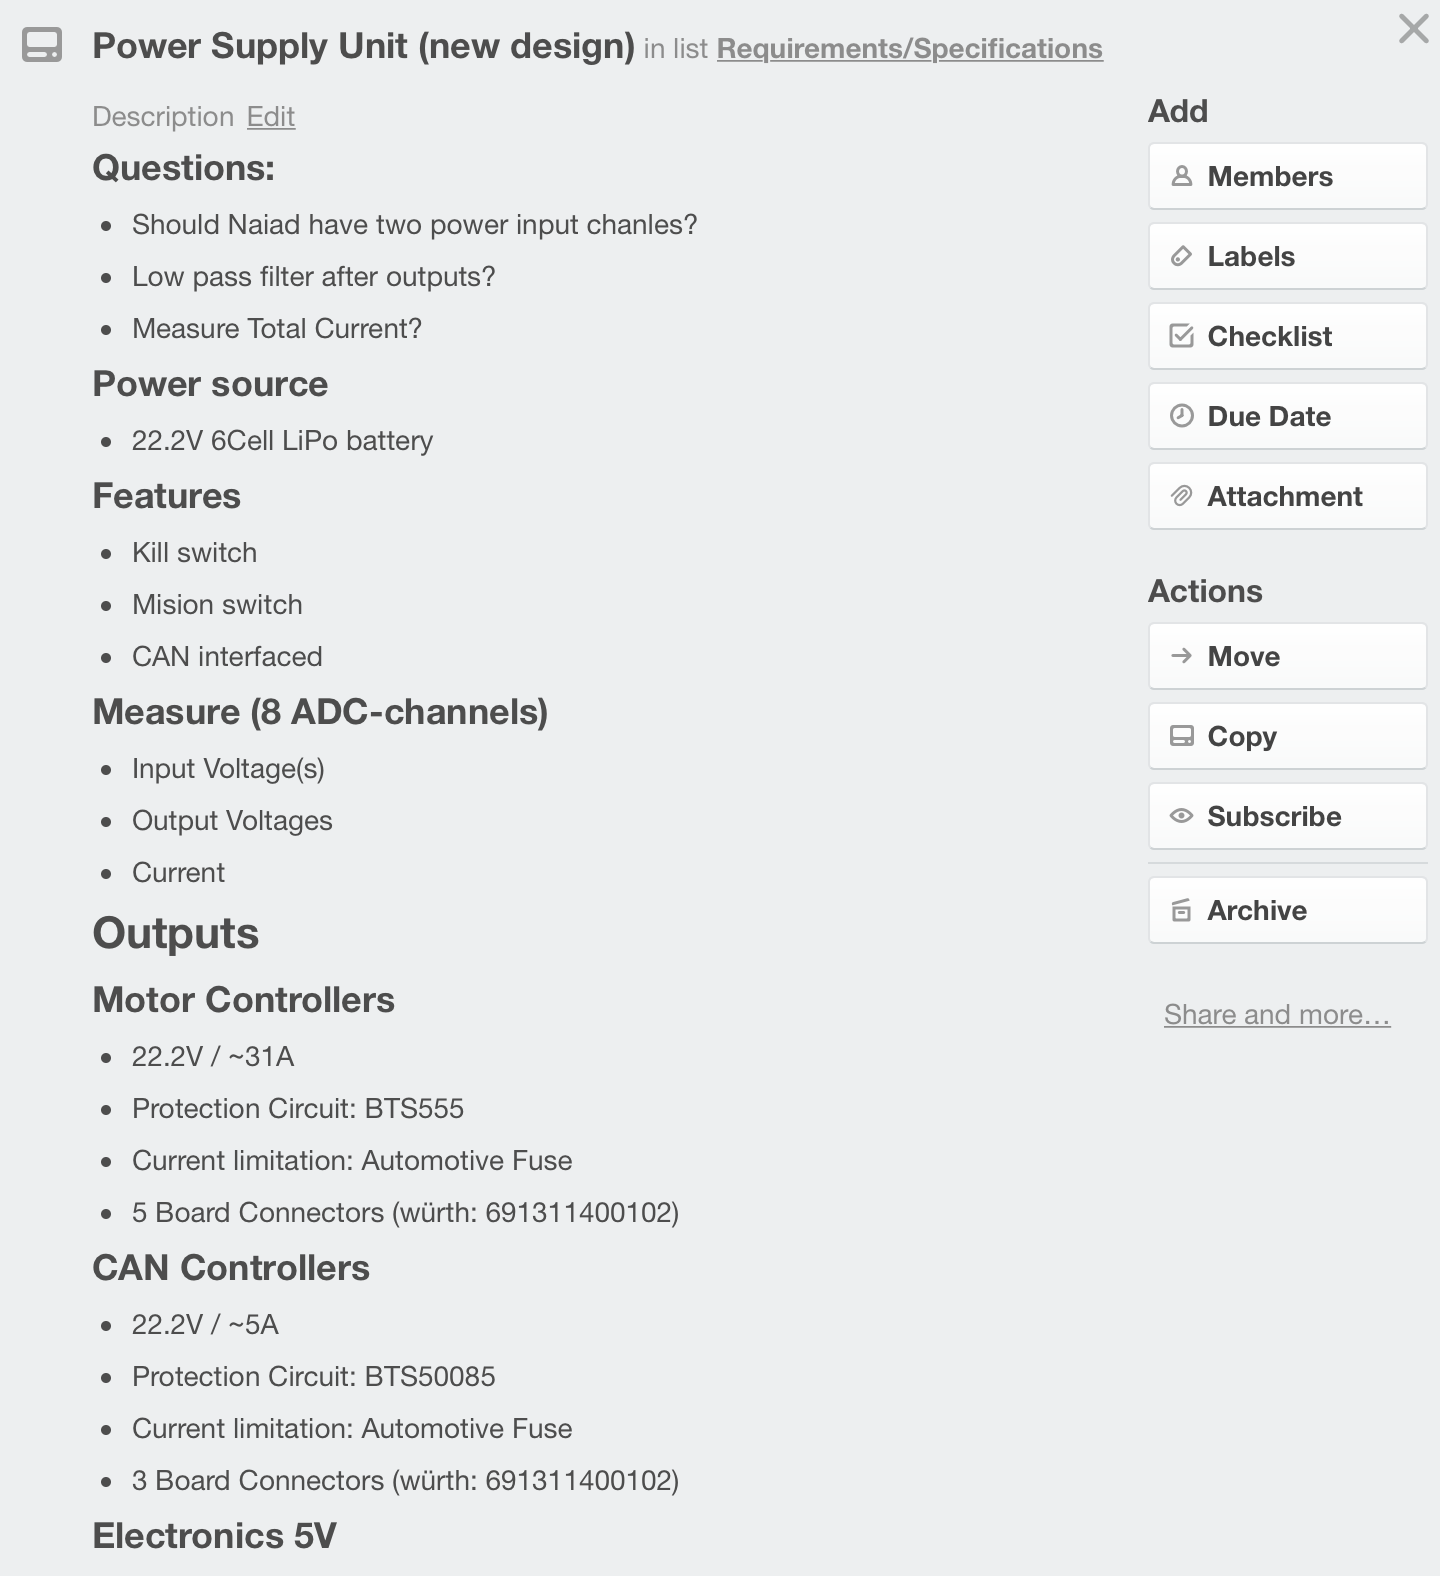
\includegraphics[scale=0.5]{Screenshoot8}

    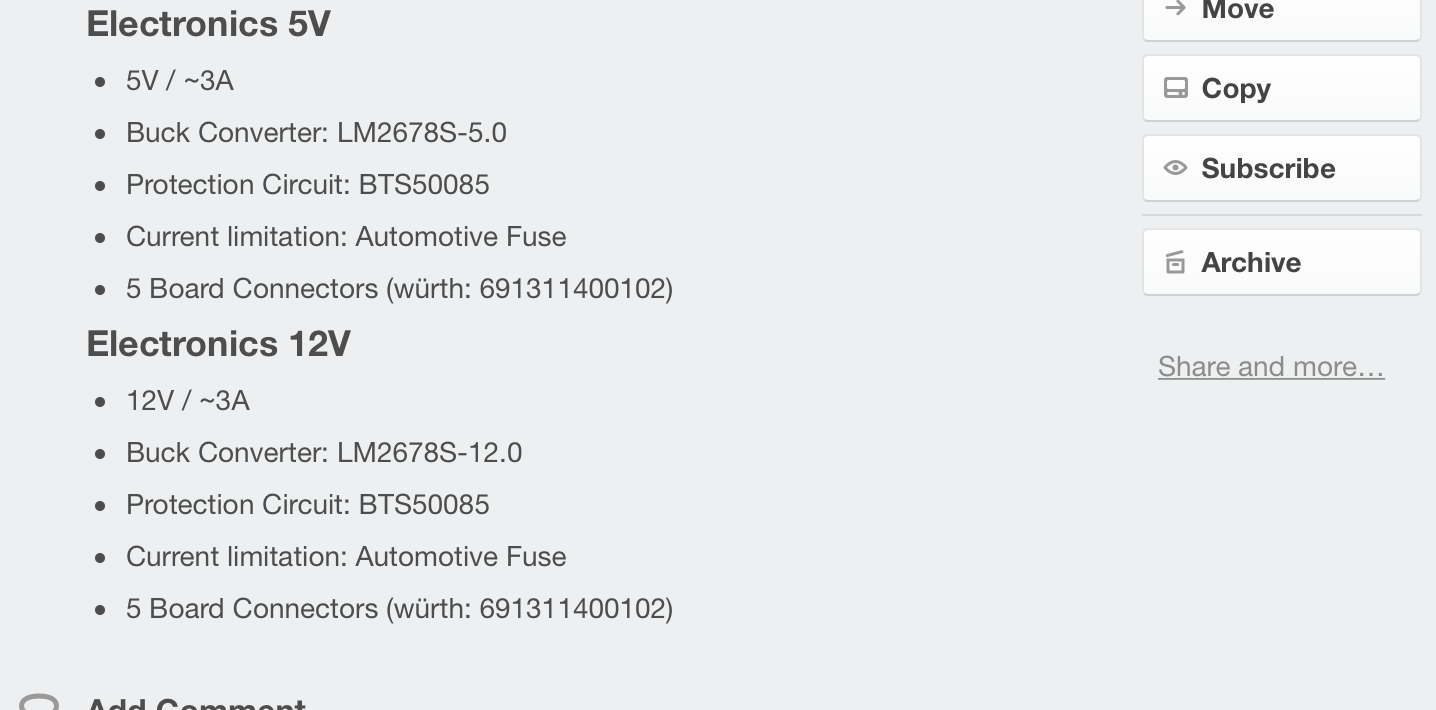
\includegraphics[scale=0.5]{Screenshoot9}

    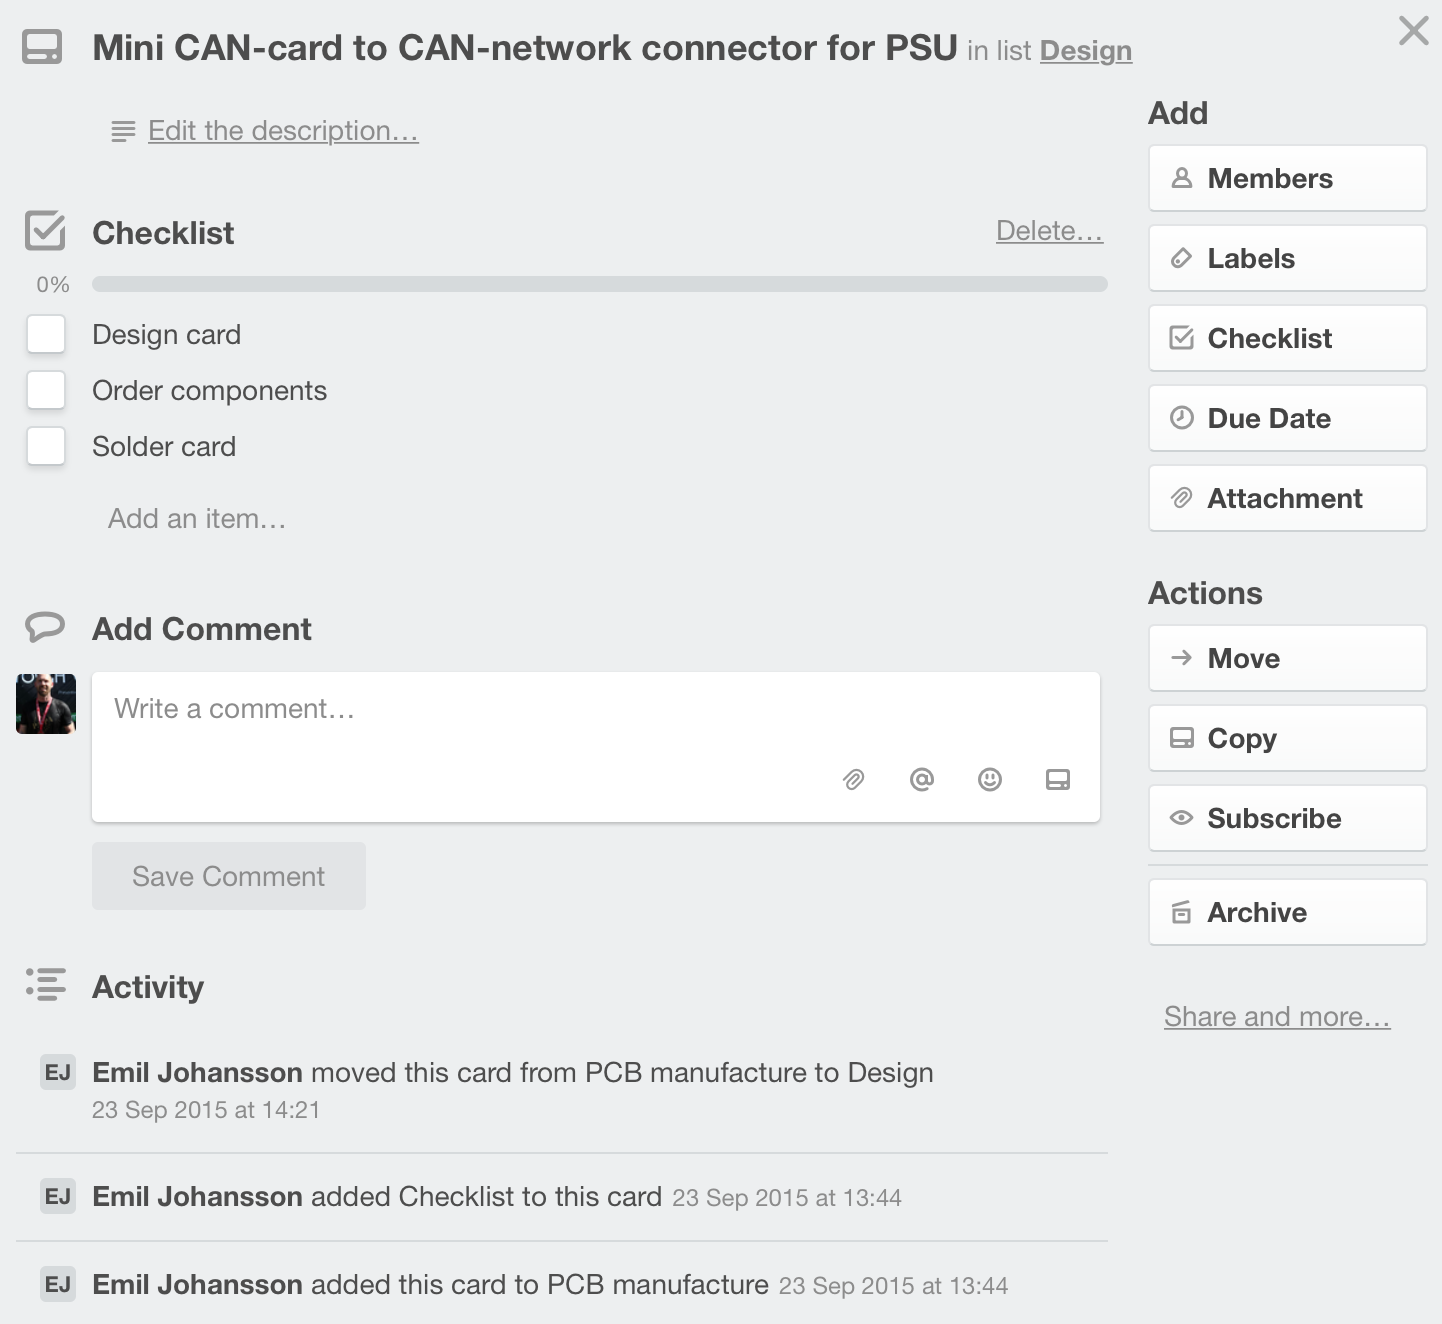
\includegraphics[scale=0.5]{Screenshoot10}

    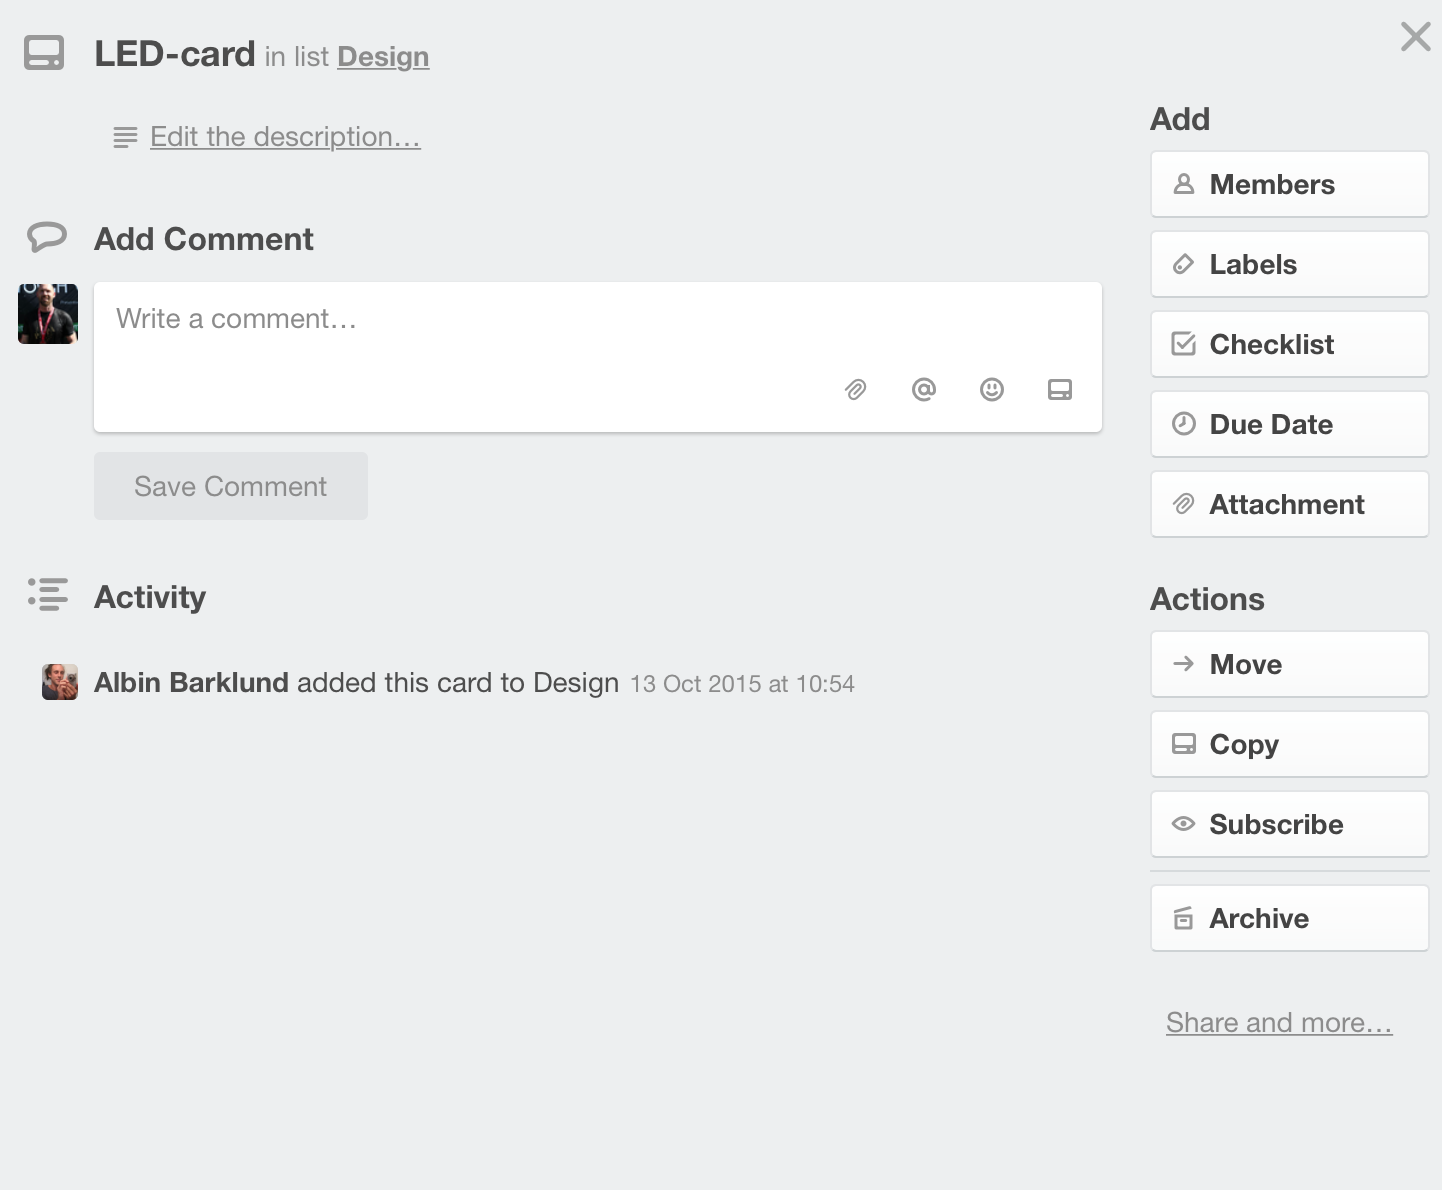
\includegraphics[scale=0.5]{Screenshoot11}

    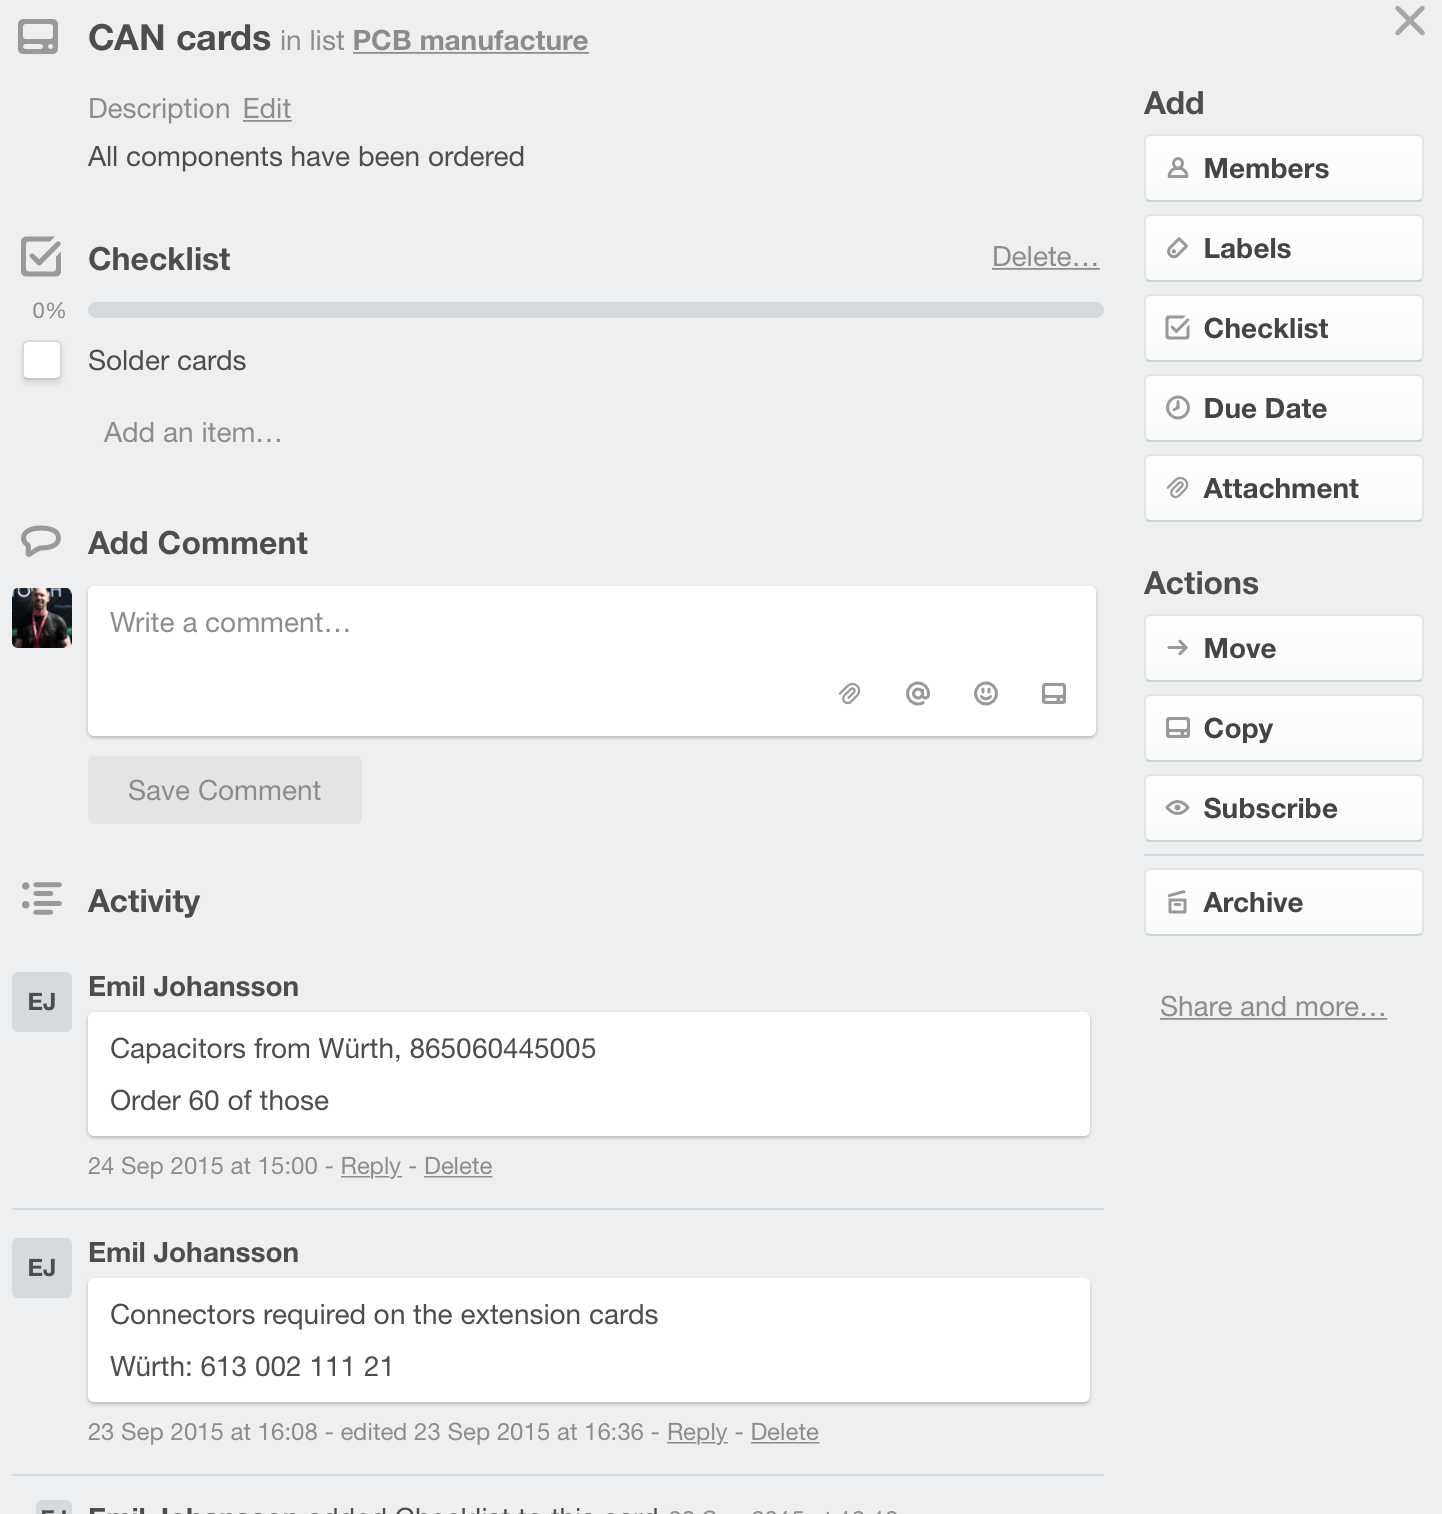
\includegraphics[scale=0.5]{Screenshoot12}

    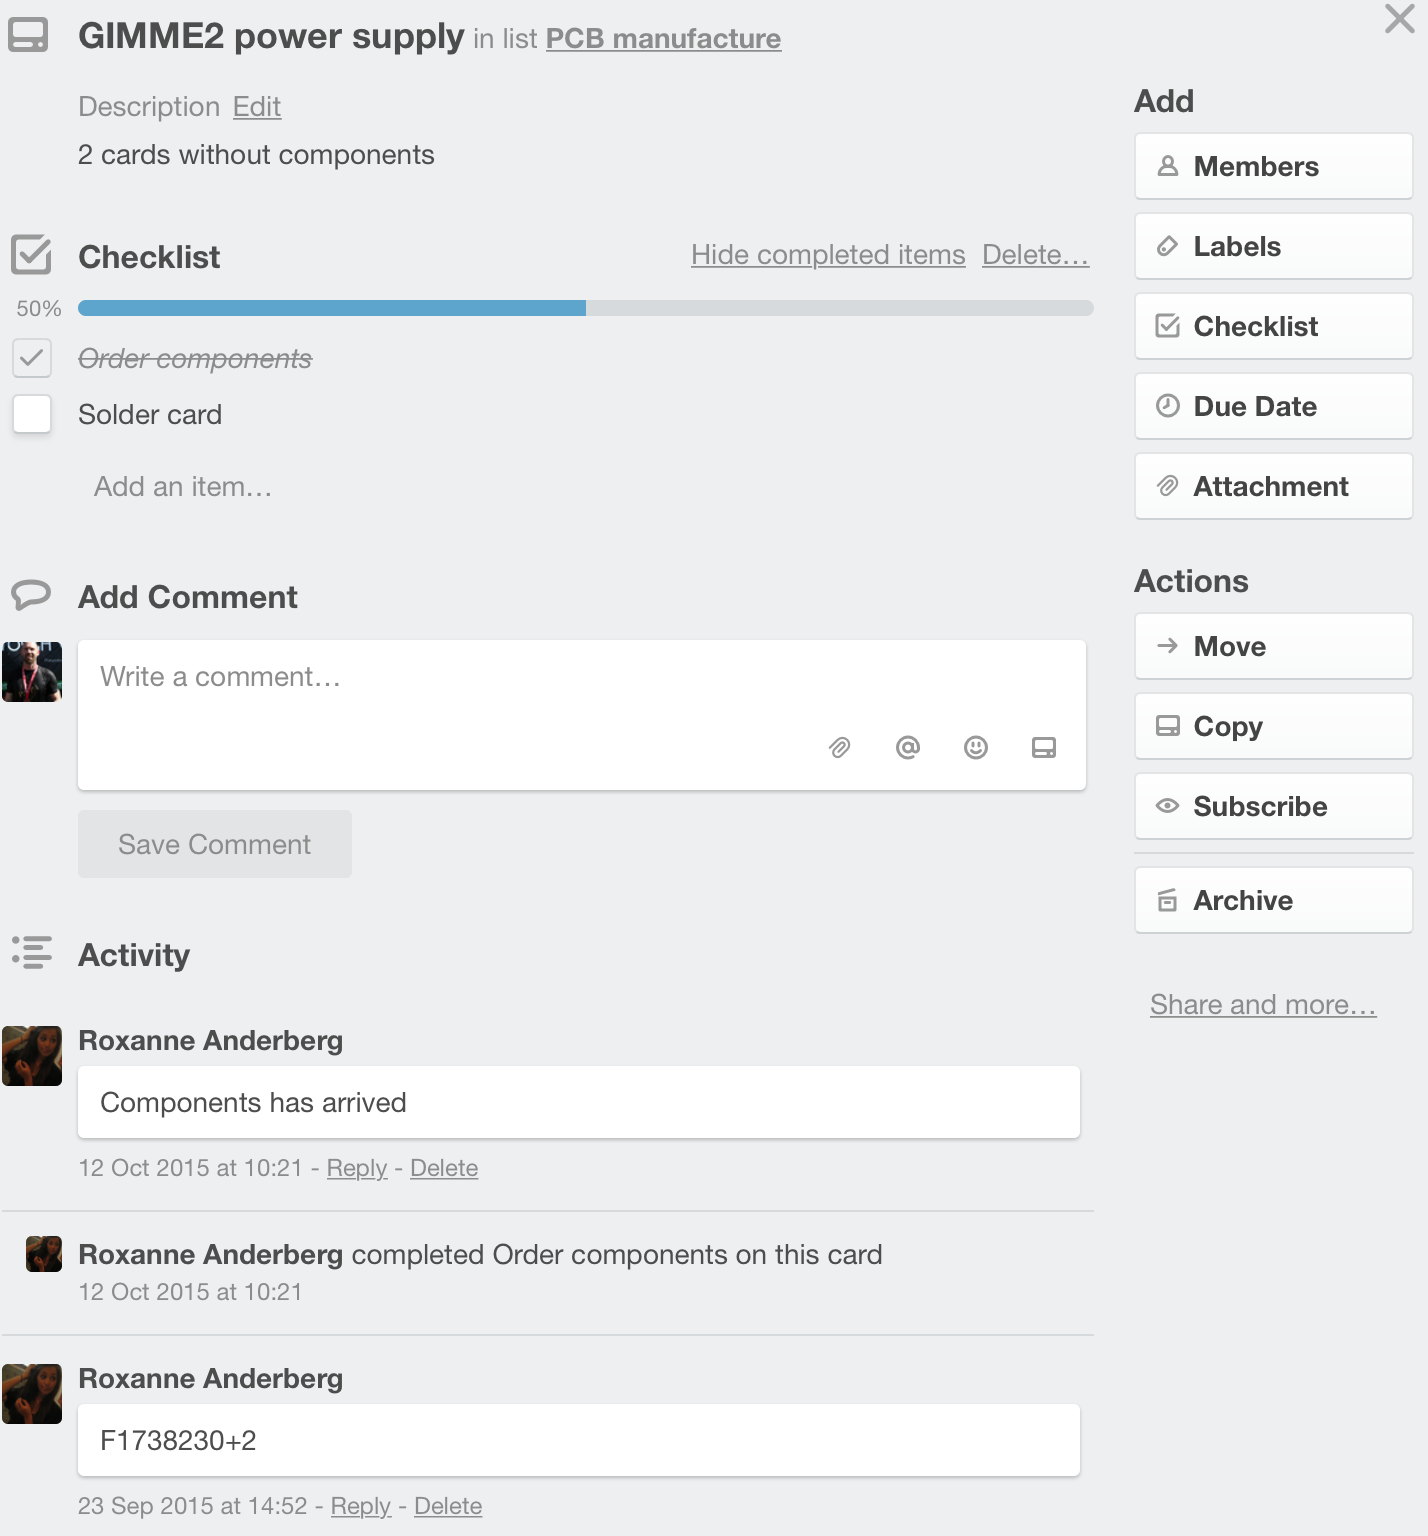
\includegraphics[scale=0.5]{Screenshoot13}

    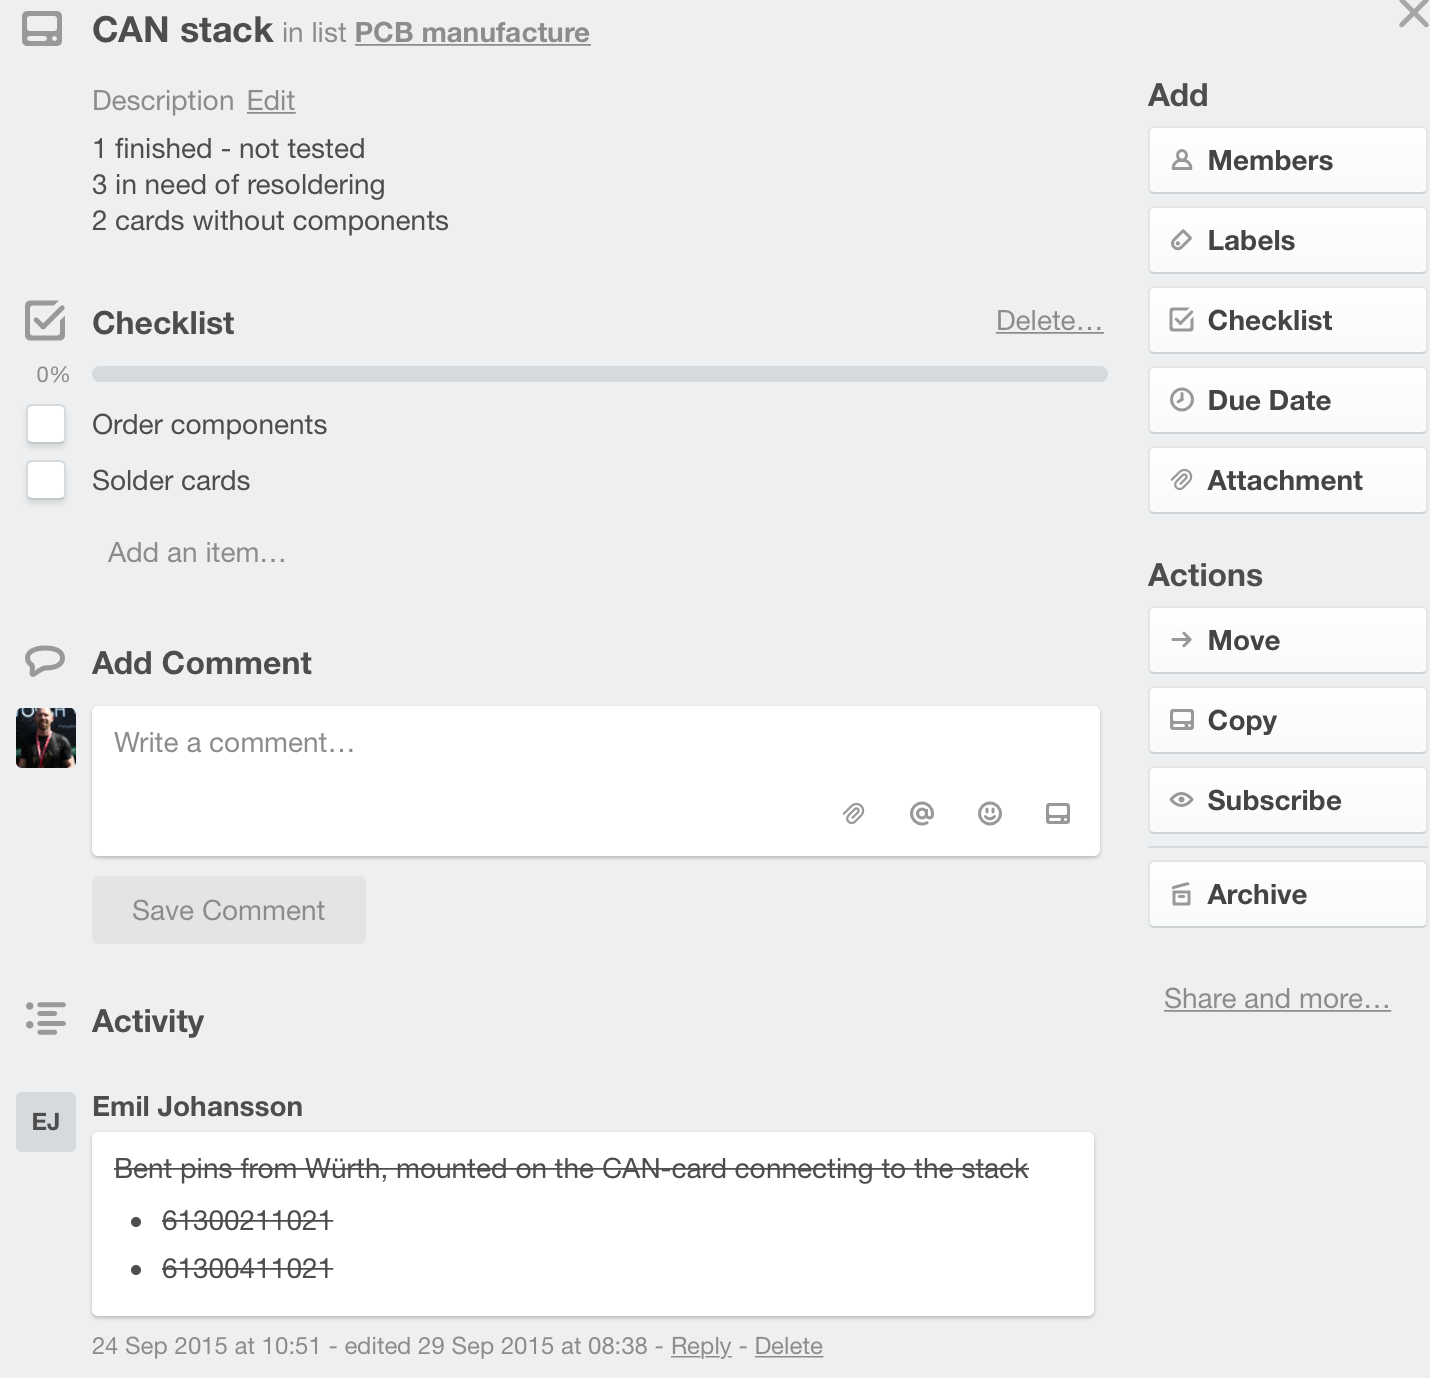
\includegraphics[scale=0.5]{Screenshoot14}

    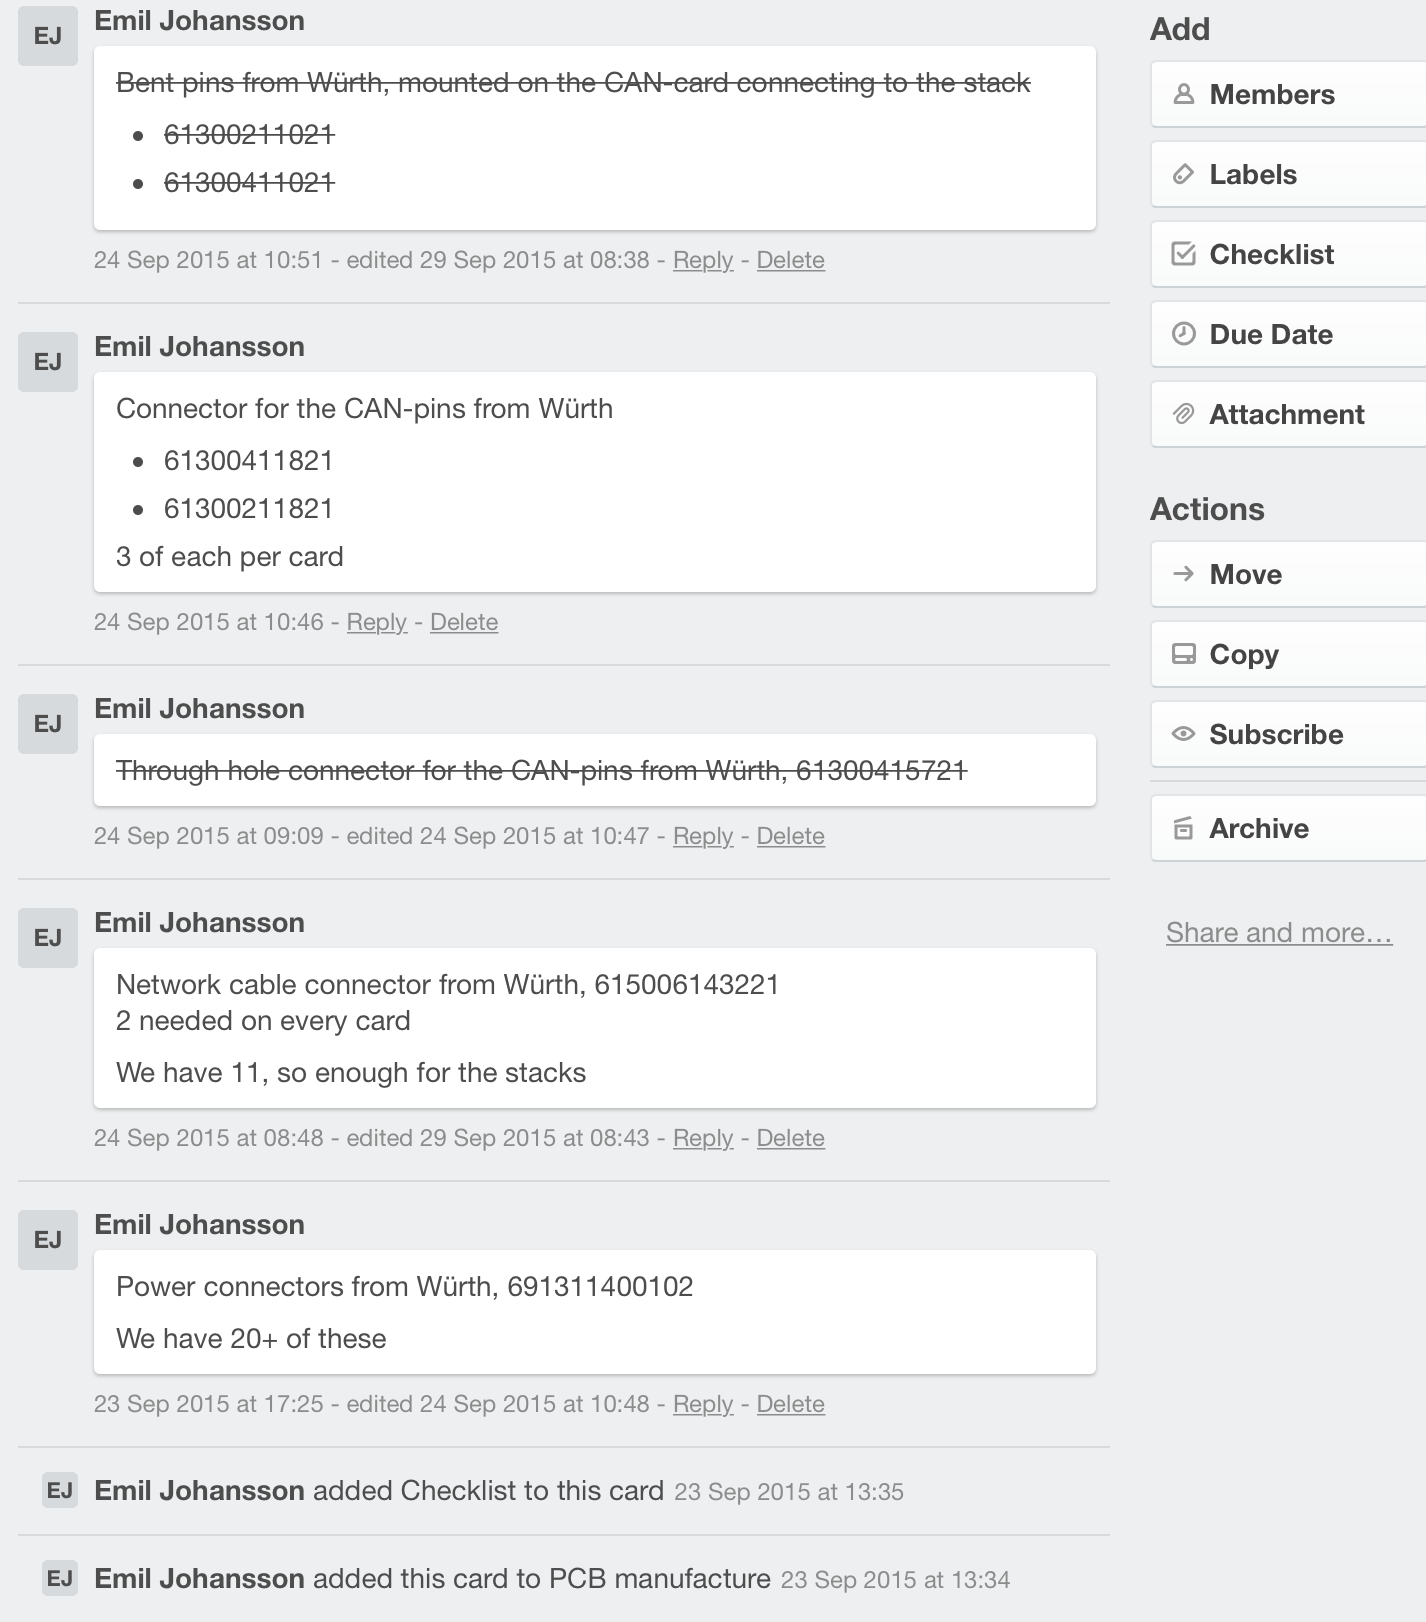
\includegraphics[scale=0.5]{Screenshoot15}

    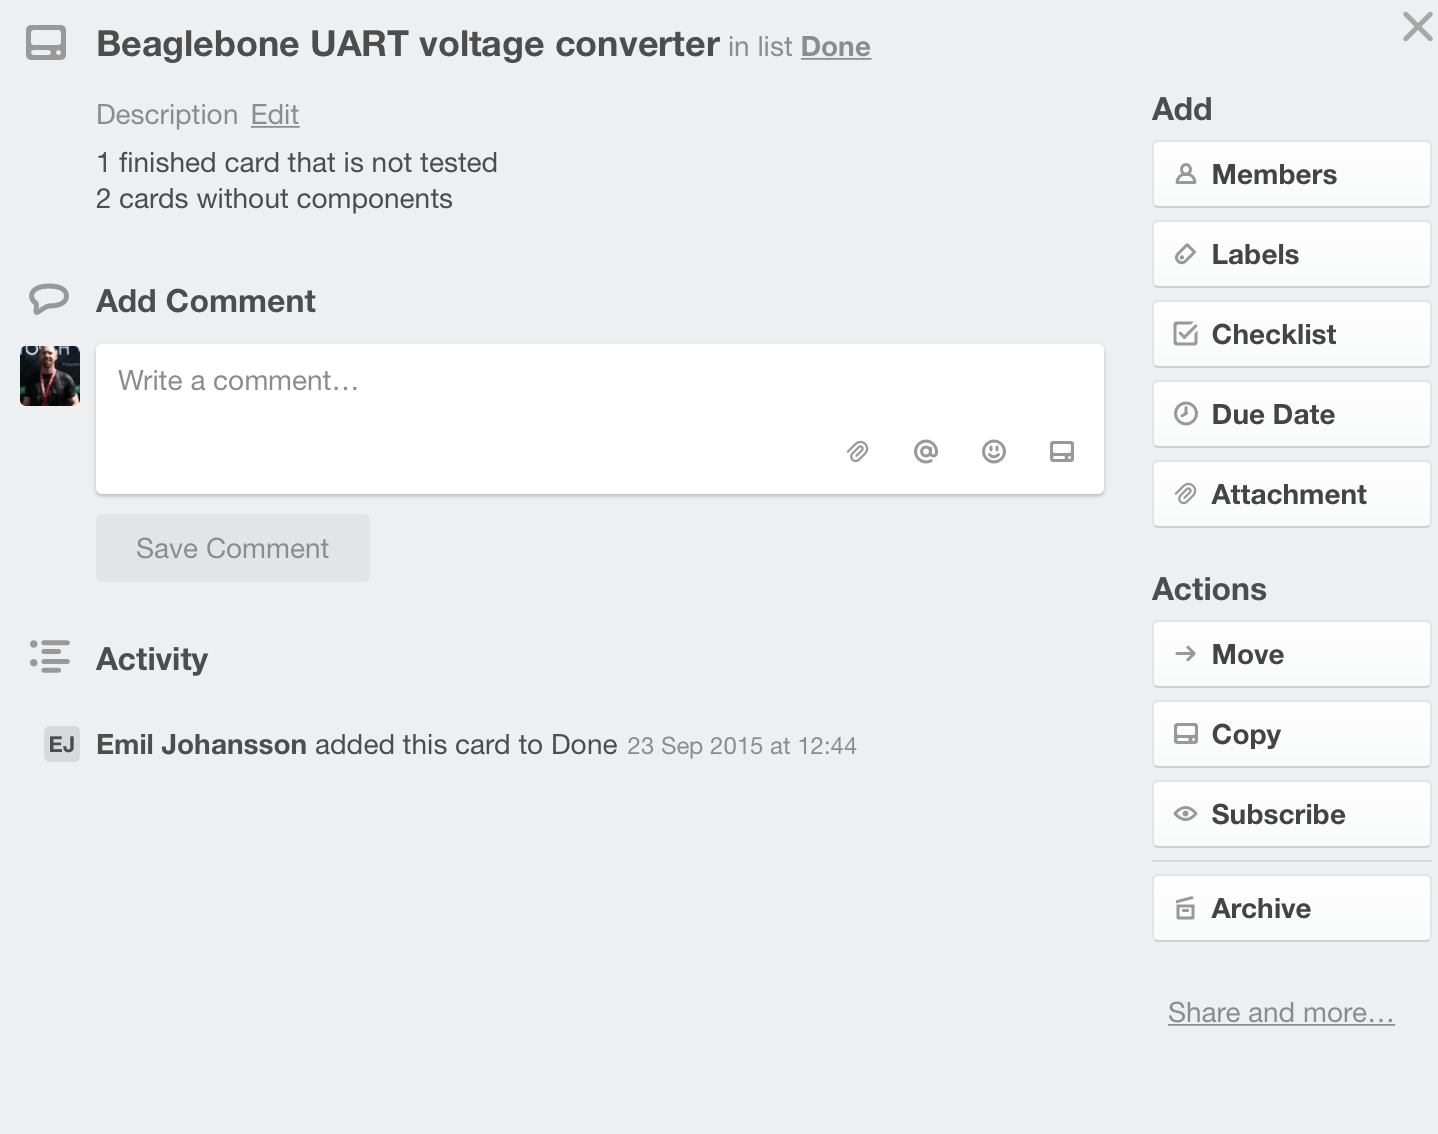
\includegraphics[scale=0.5]{Screenshoot16}

    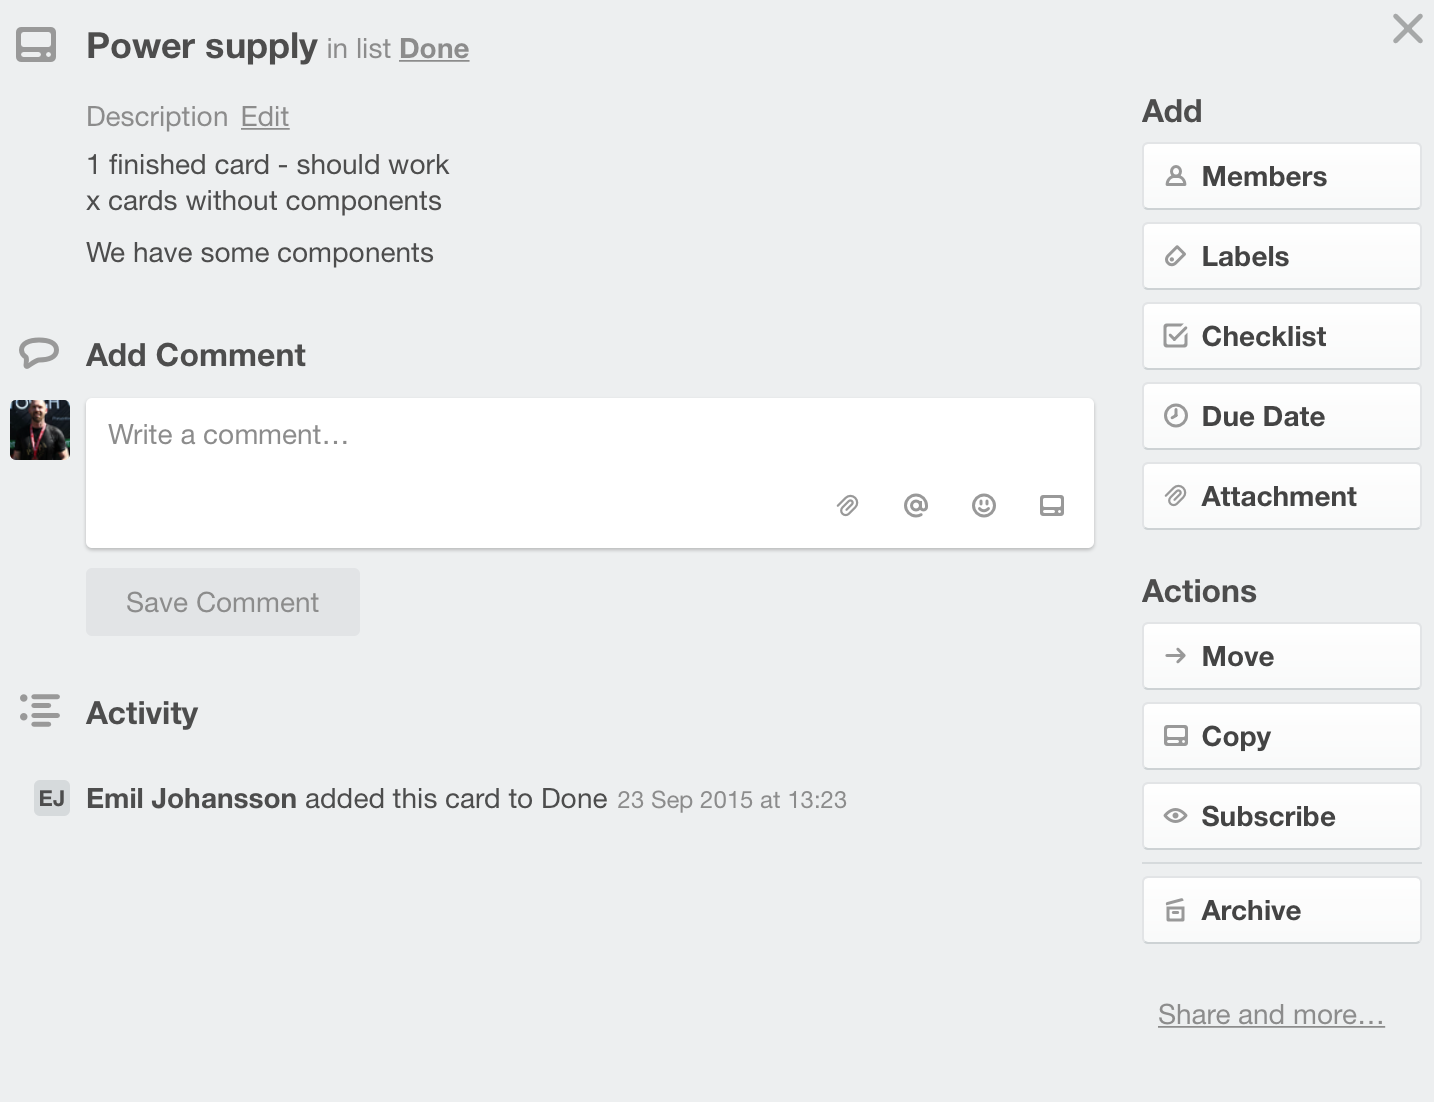
\includegraphics[scale=0.5]{Screenshoot17}

    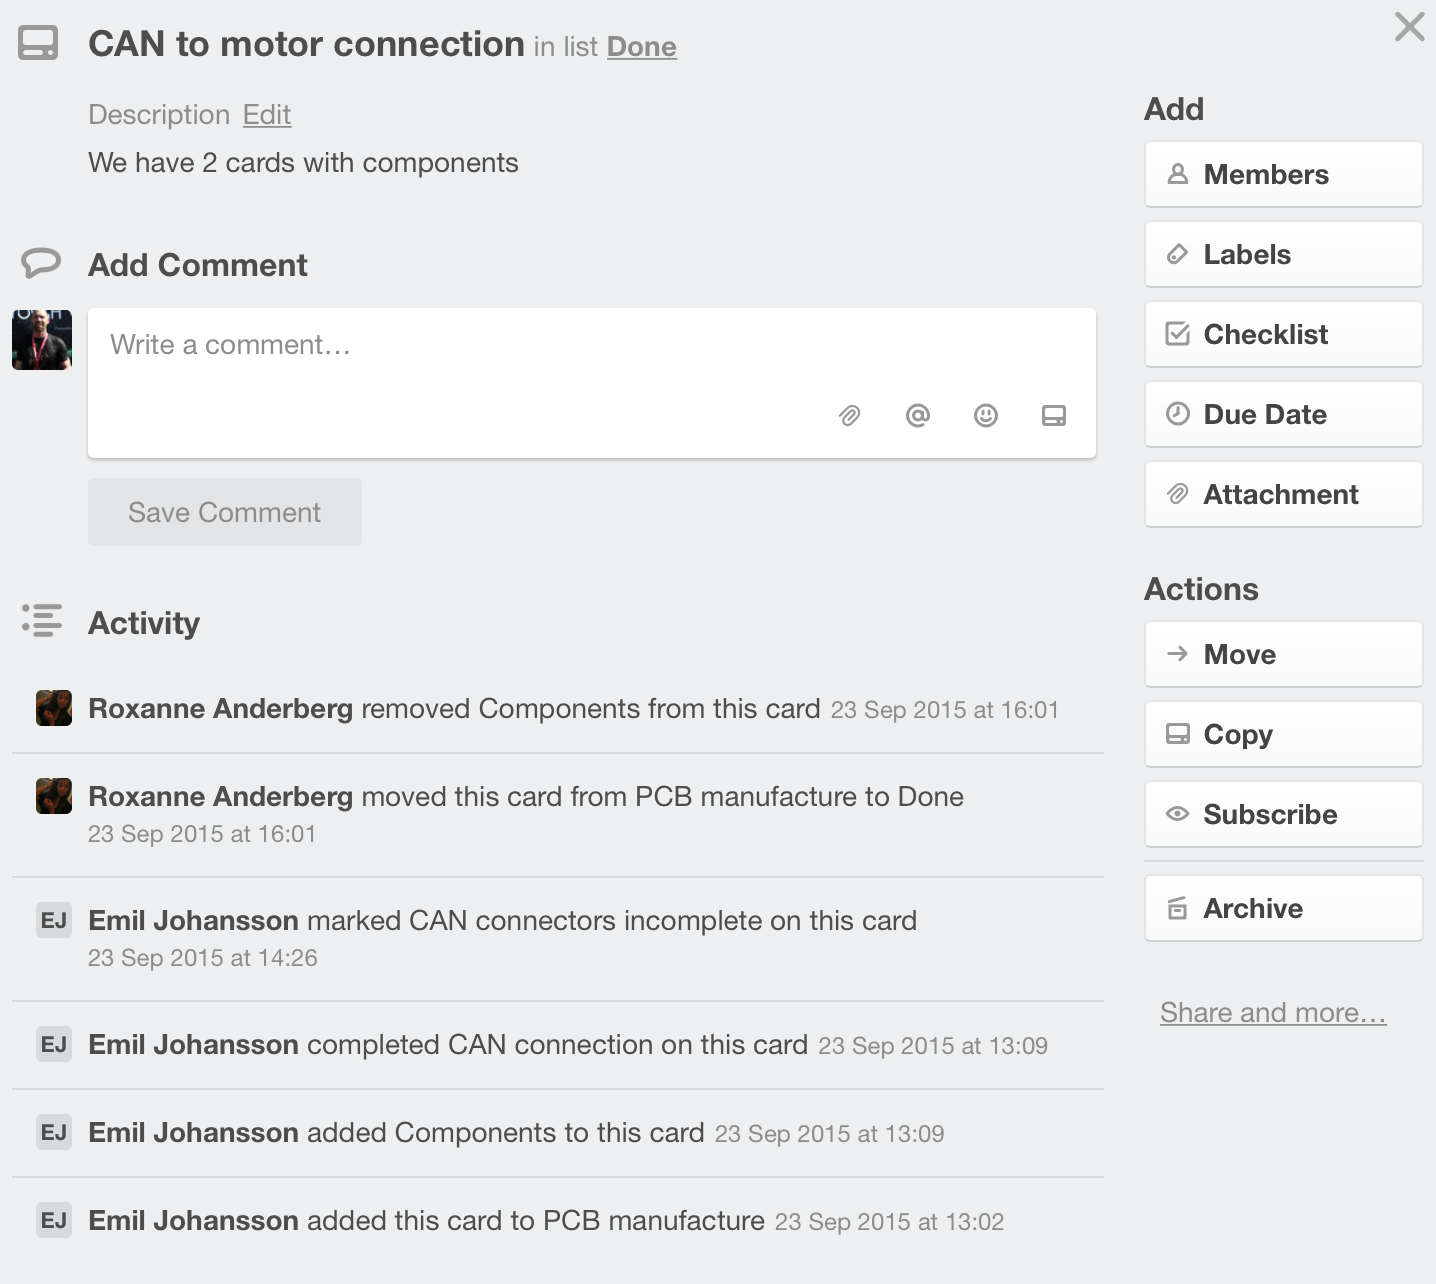
\includegraphics[scale=0.5]{Screenshoot18}

    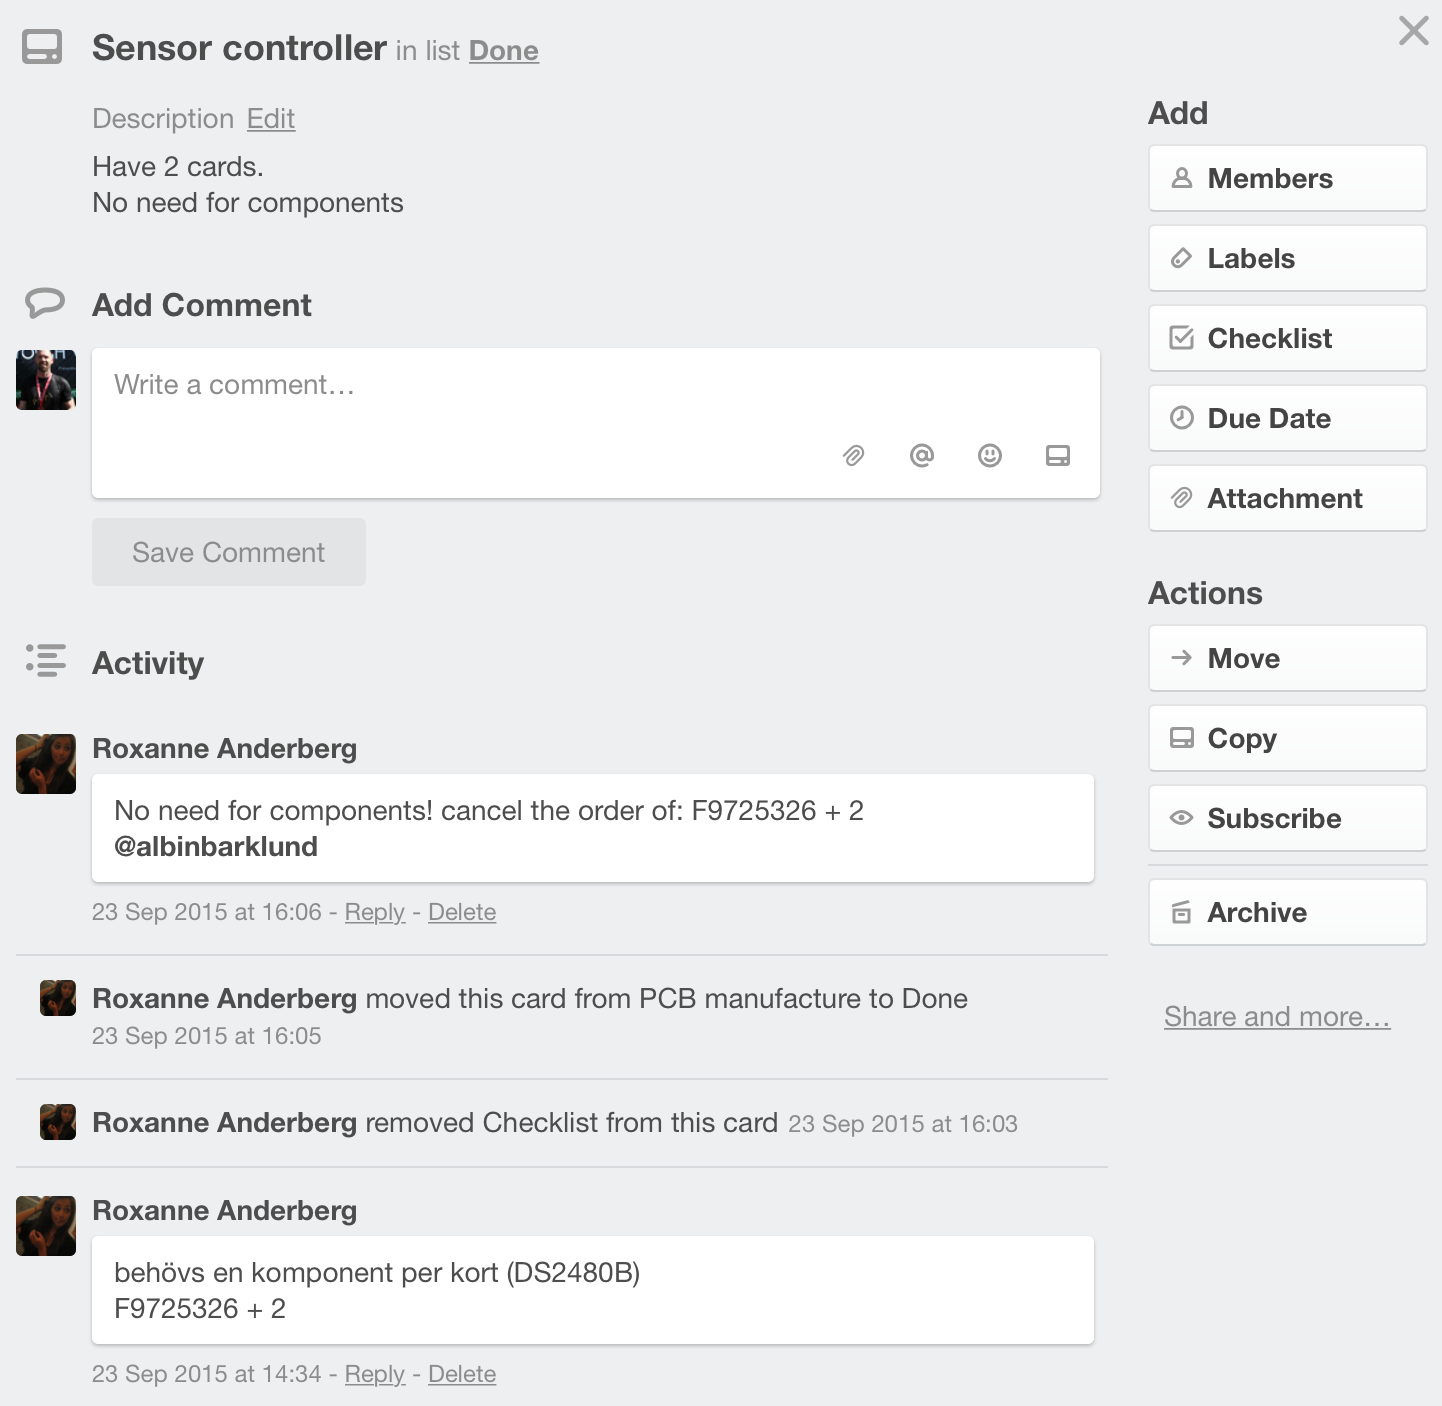
\includegraphics[scale=0.5]{Screenshoot19}

    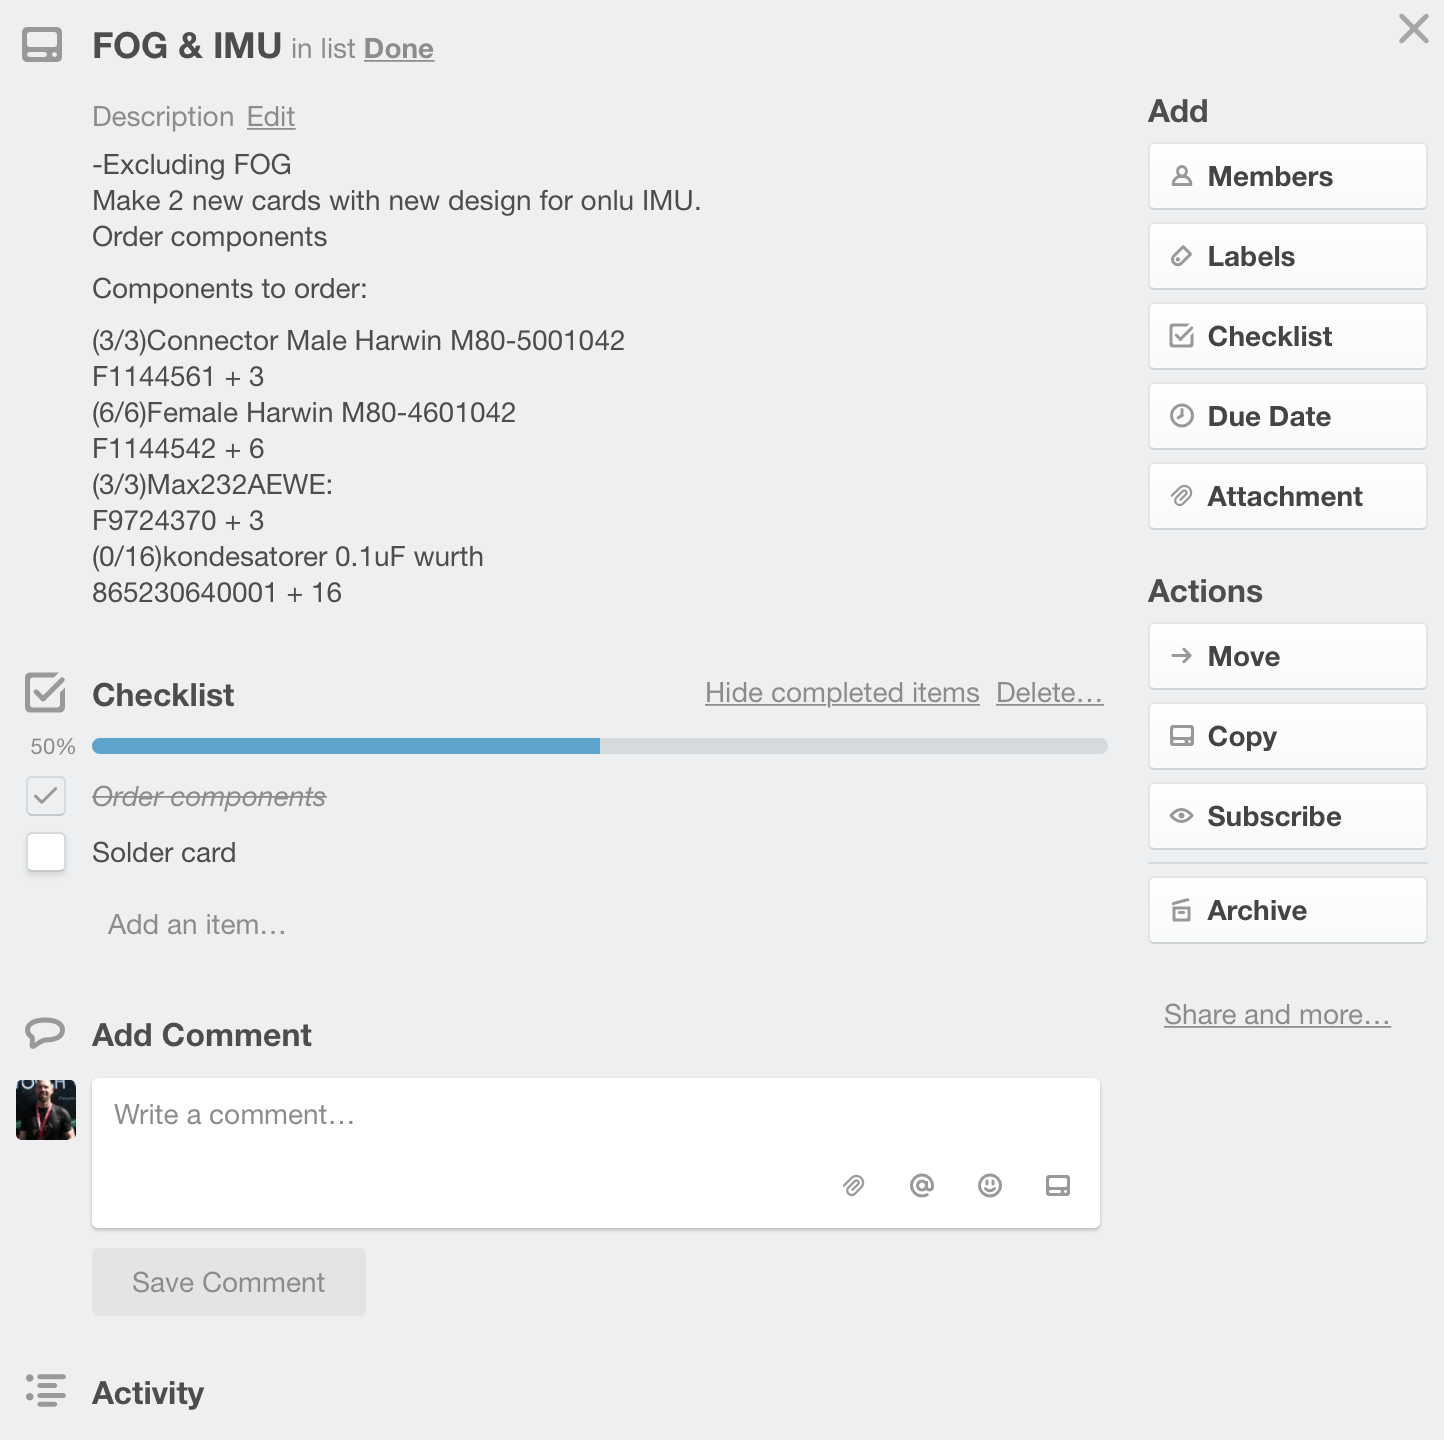
\includegraphics[scale=0.5]{Screenshoot20}

    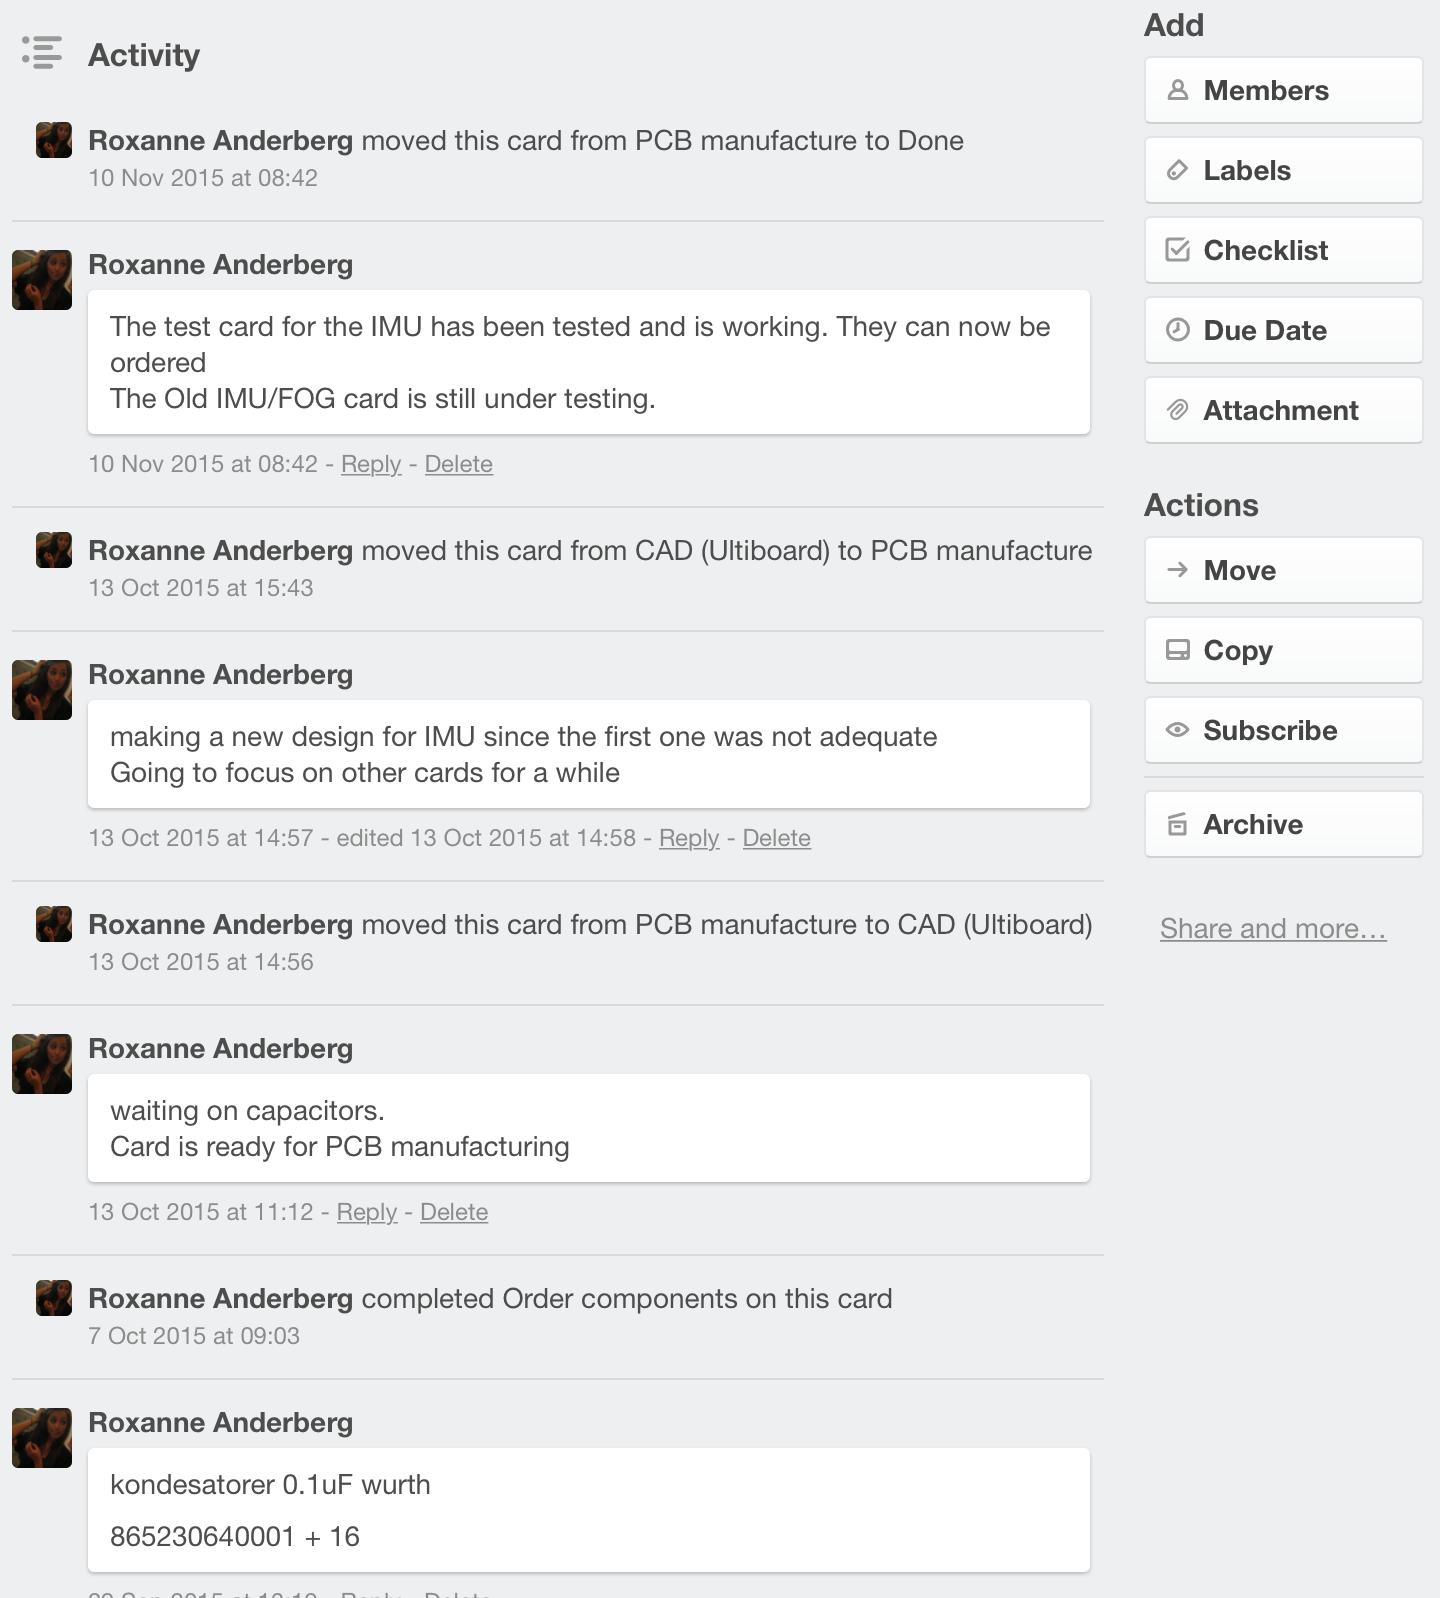
\includegraphics[scale=0.5]{Screenshoot21}

    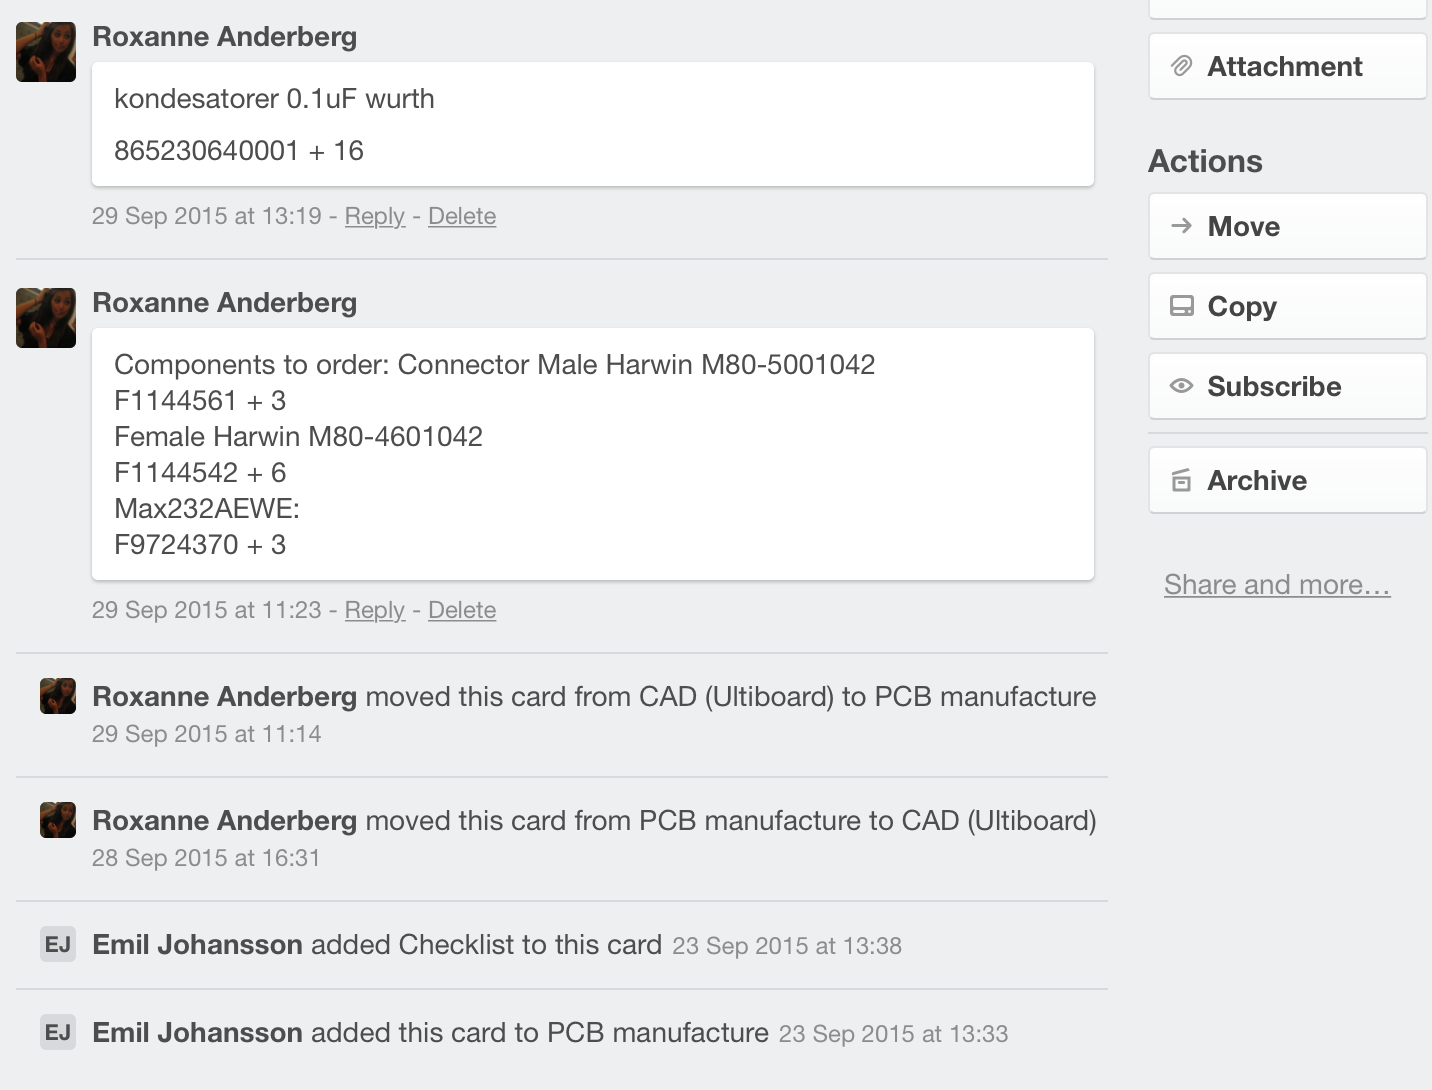
\includegraphics[scale=0.5]{Screenshoot22}

    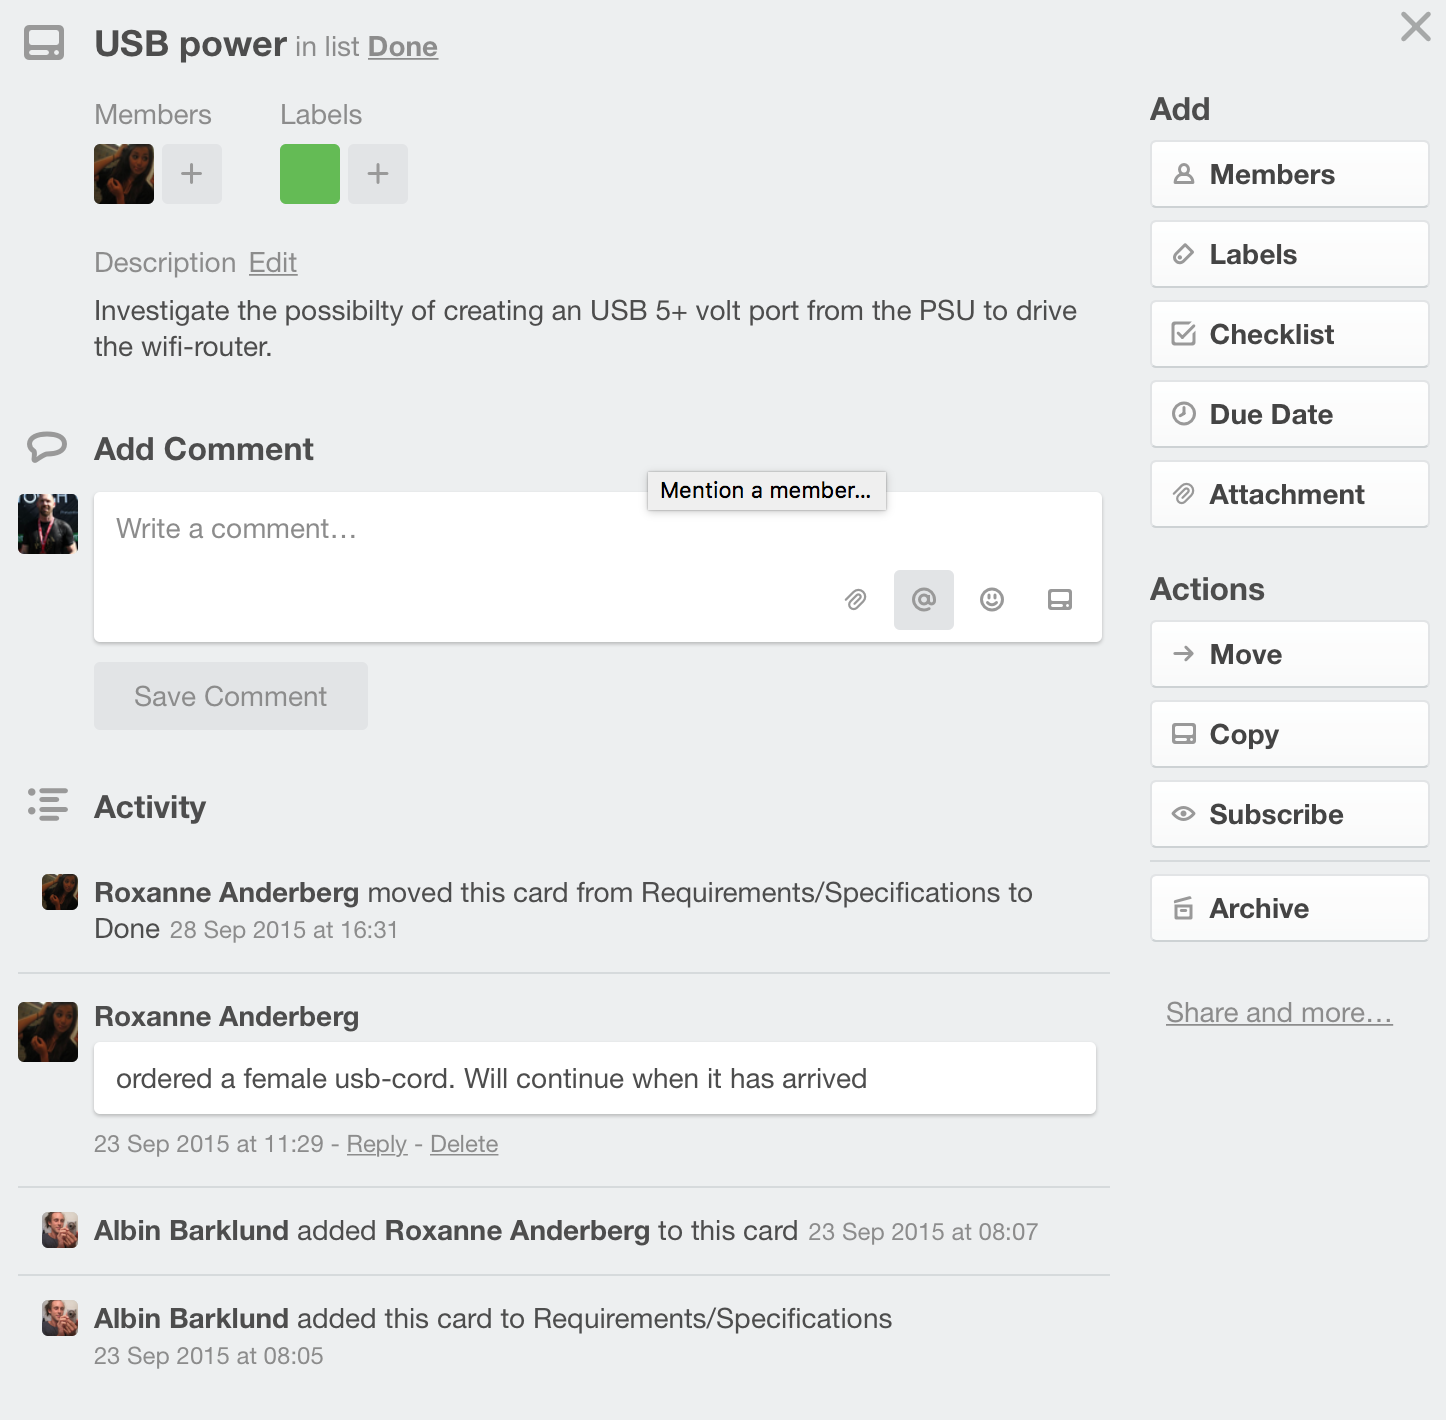
\includegraphics[scale=0.5]{Screenshoot23}



\newpage
\subsection{Mechanics trello Cards}

    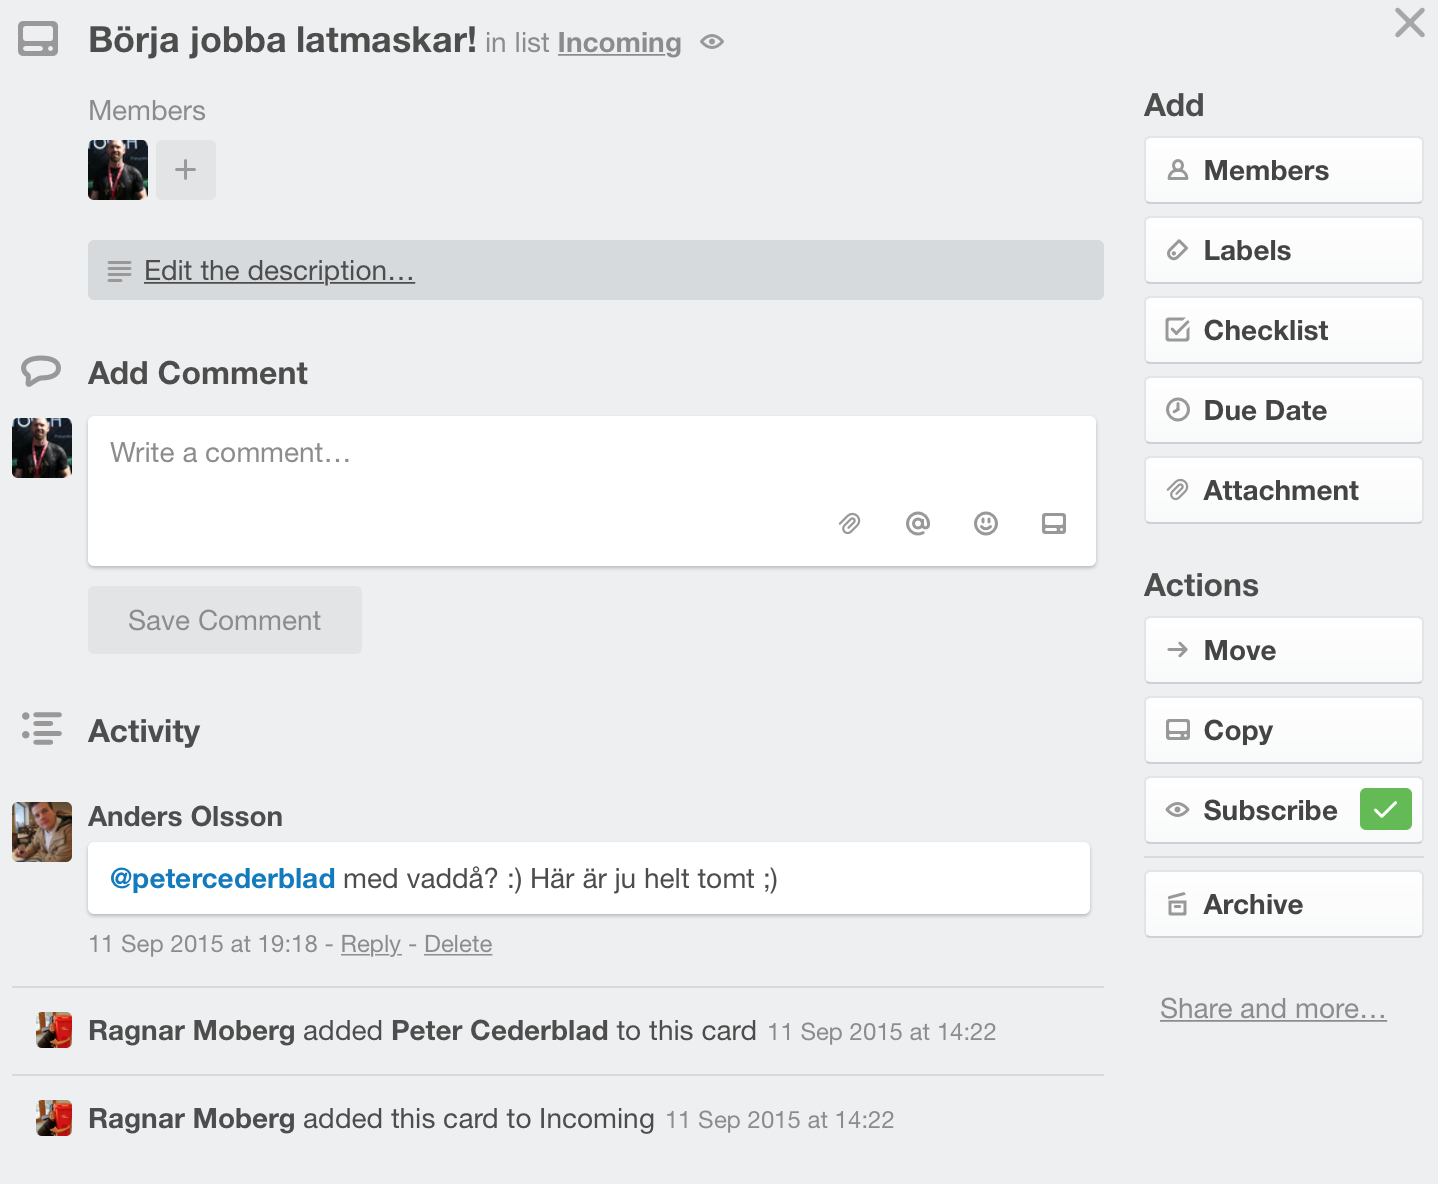
\includegraphics[scale=0.5]{Screenshoot24}

    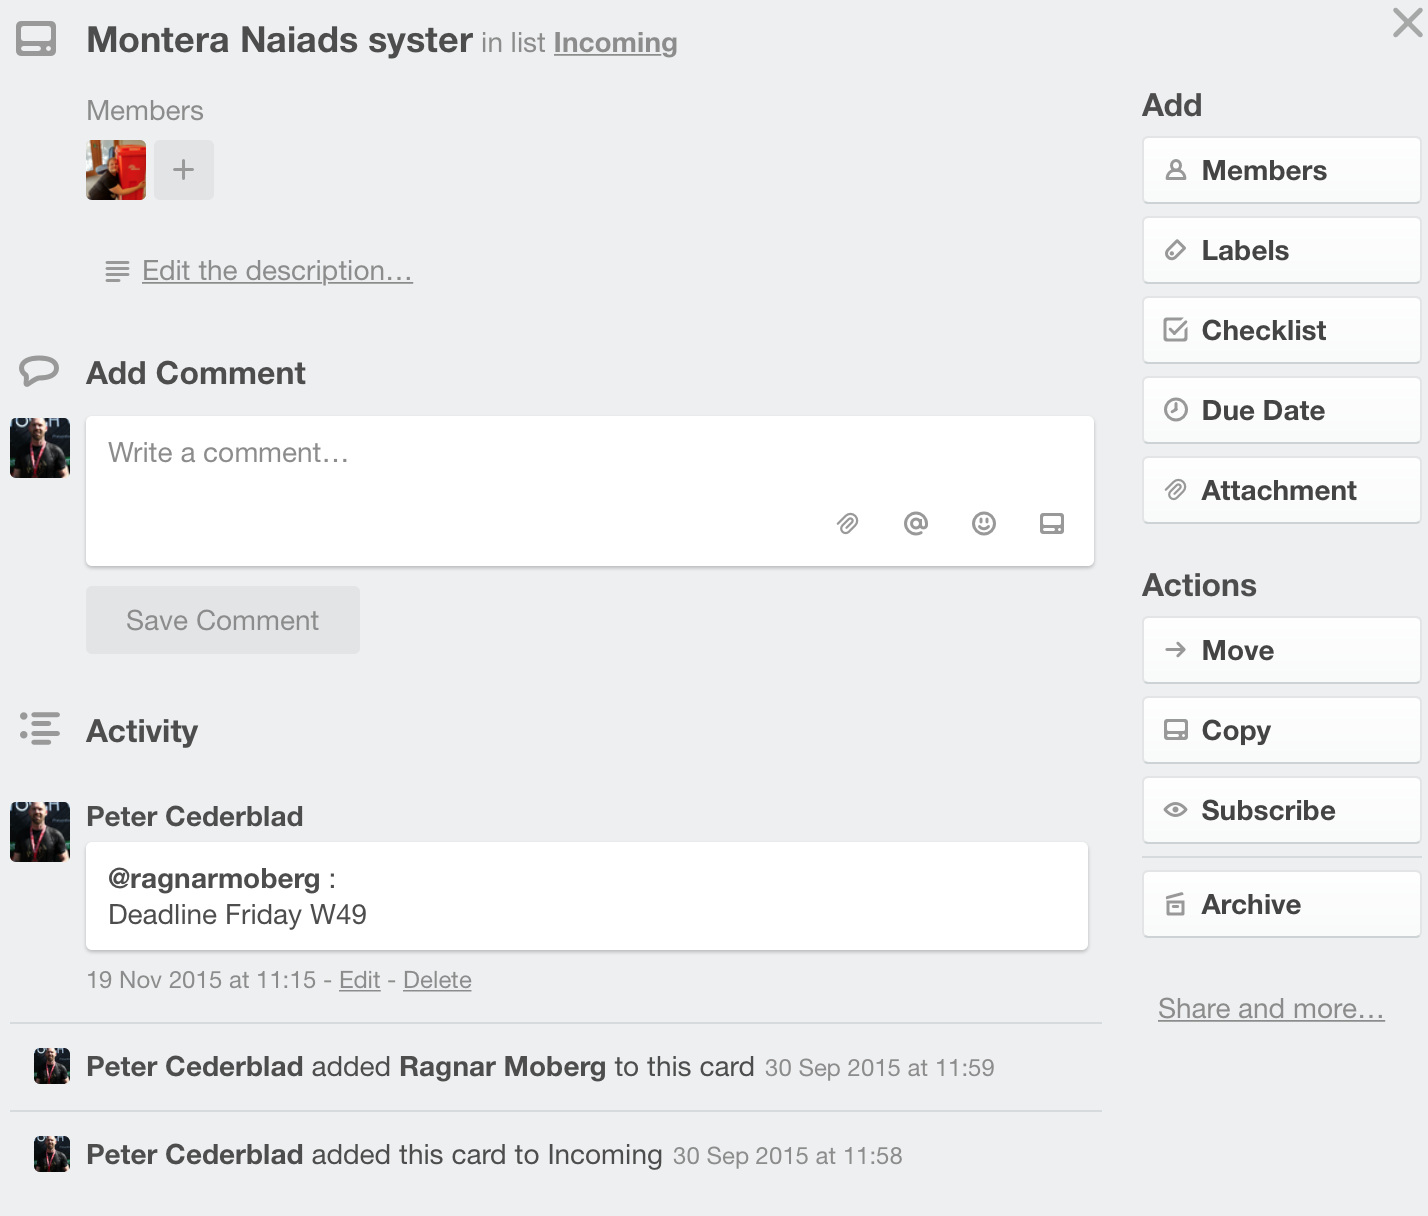
\includegraphics[scale=0.5]{Screenshoot25}

    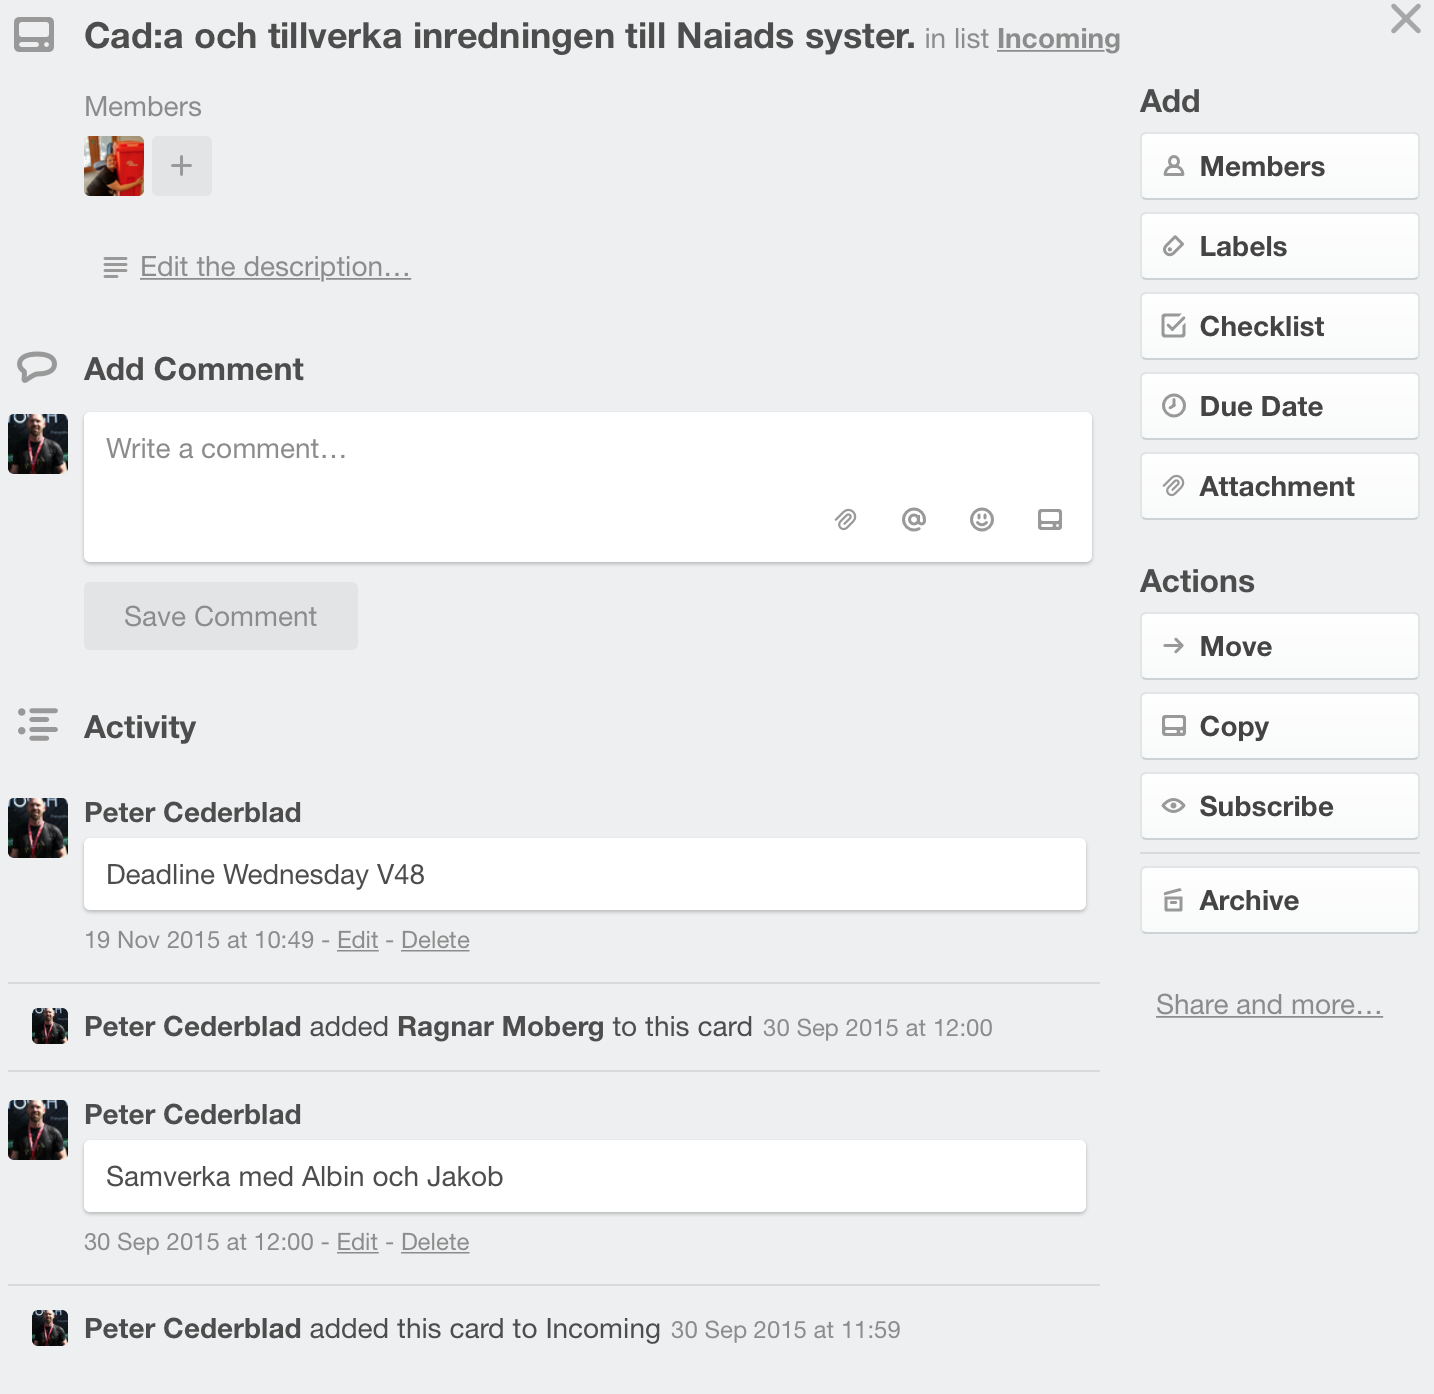
\includegraphics[scale=0.5]{Screenshoot26}

    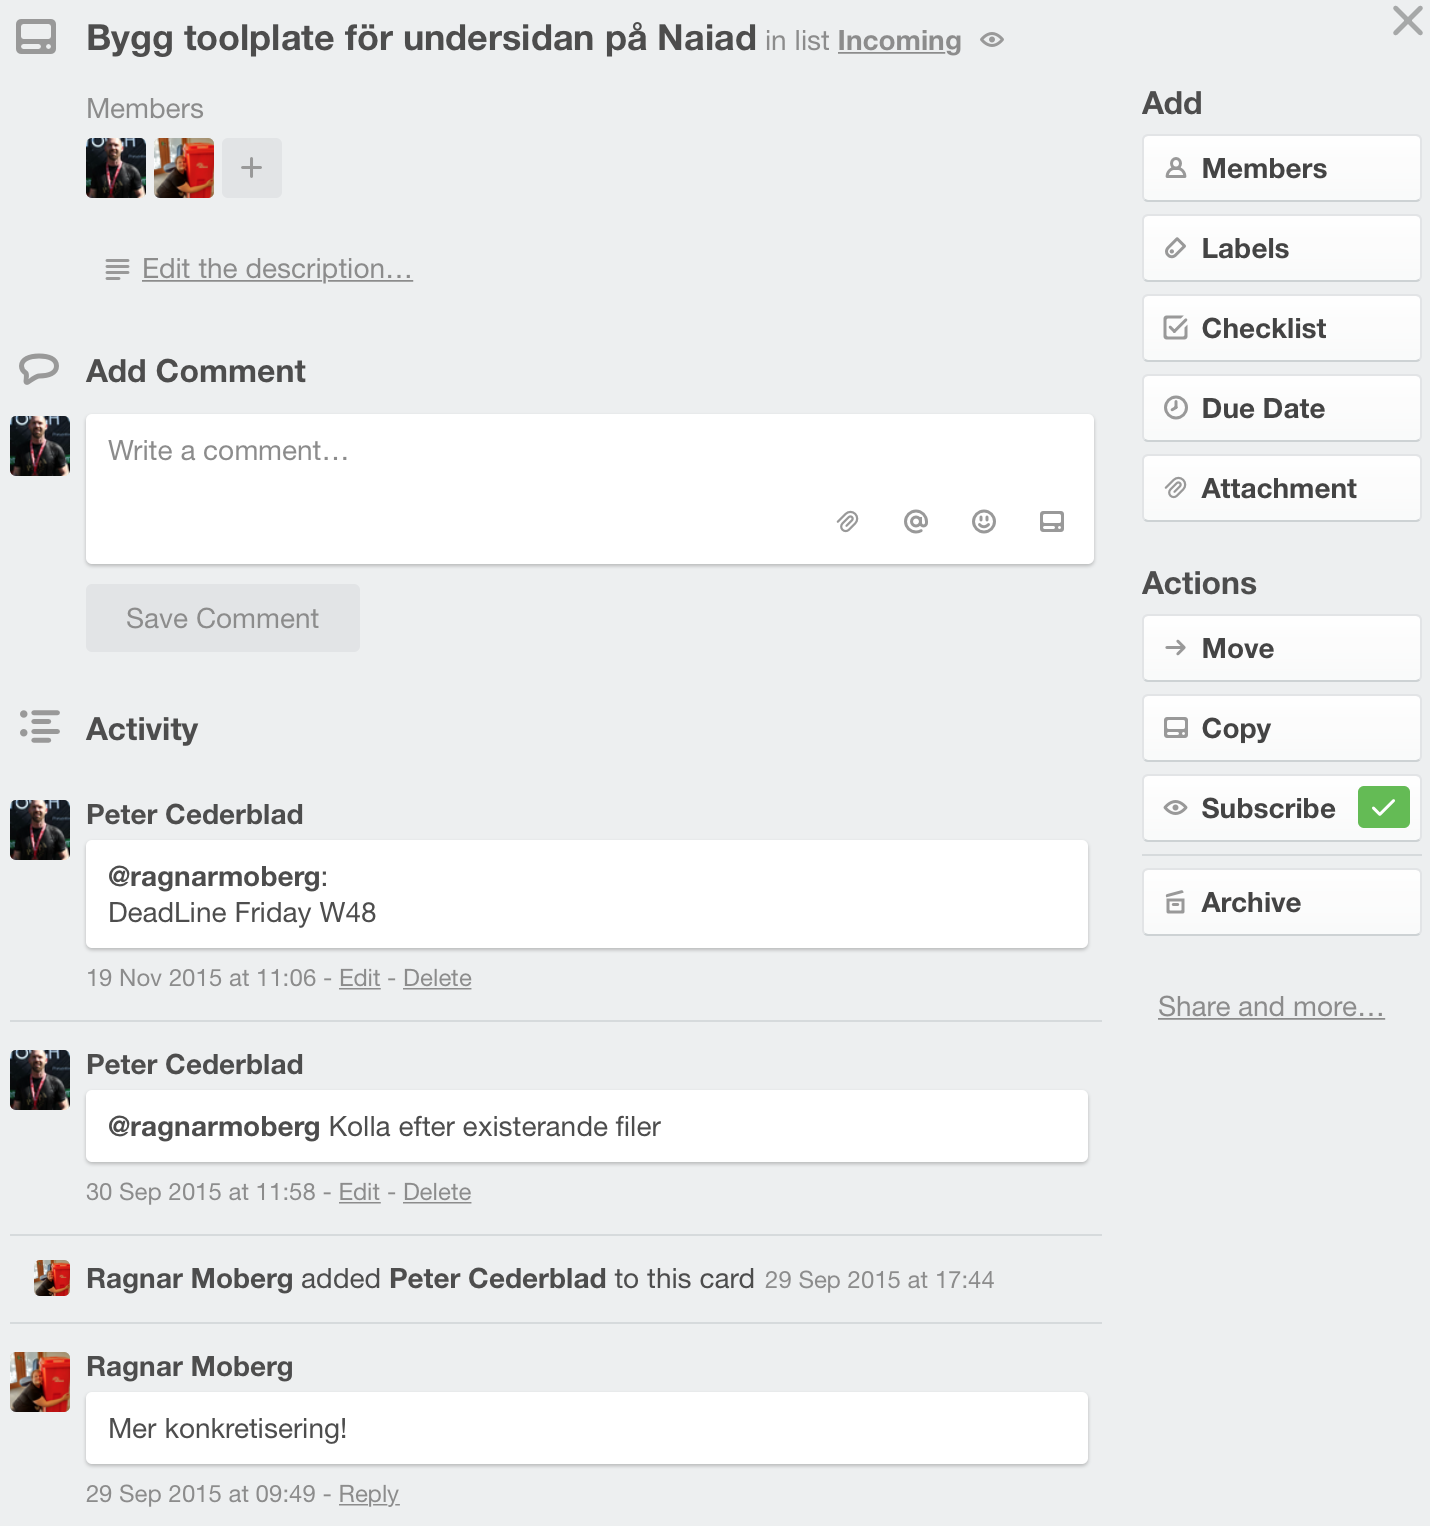
\includegraphics[scale=0.5]{Screenshoot27}

    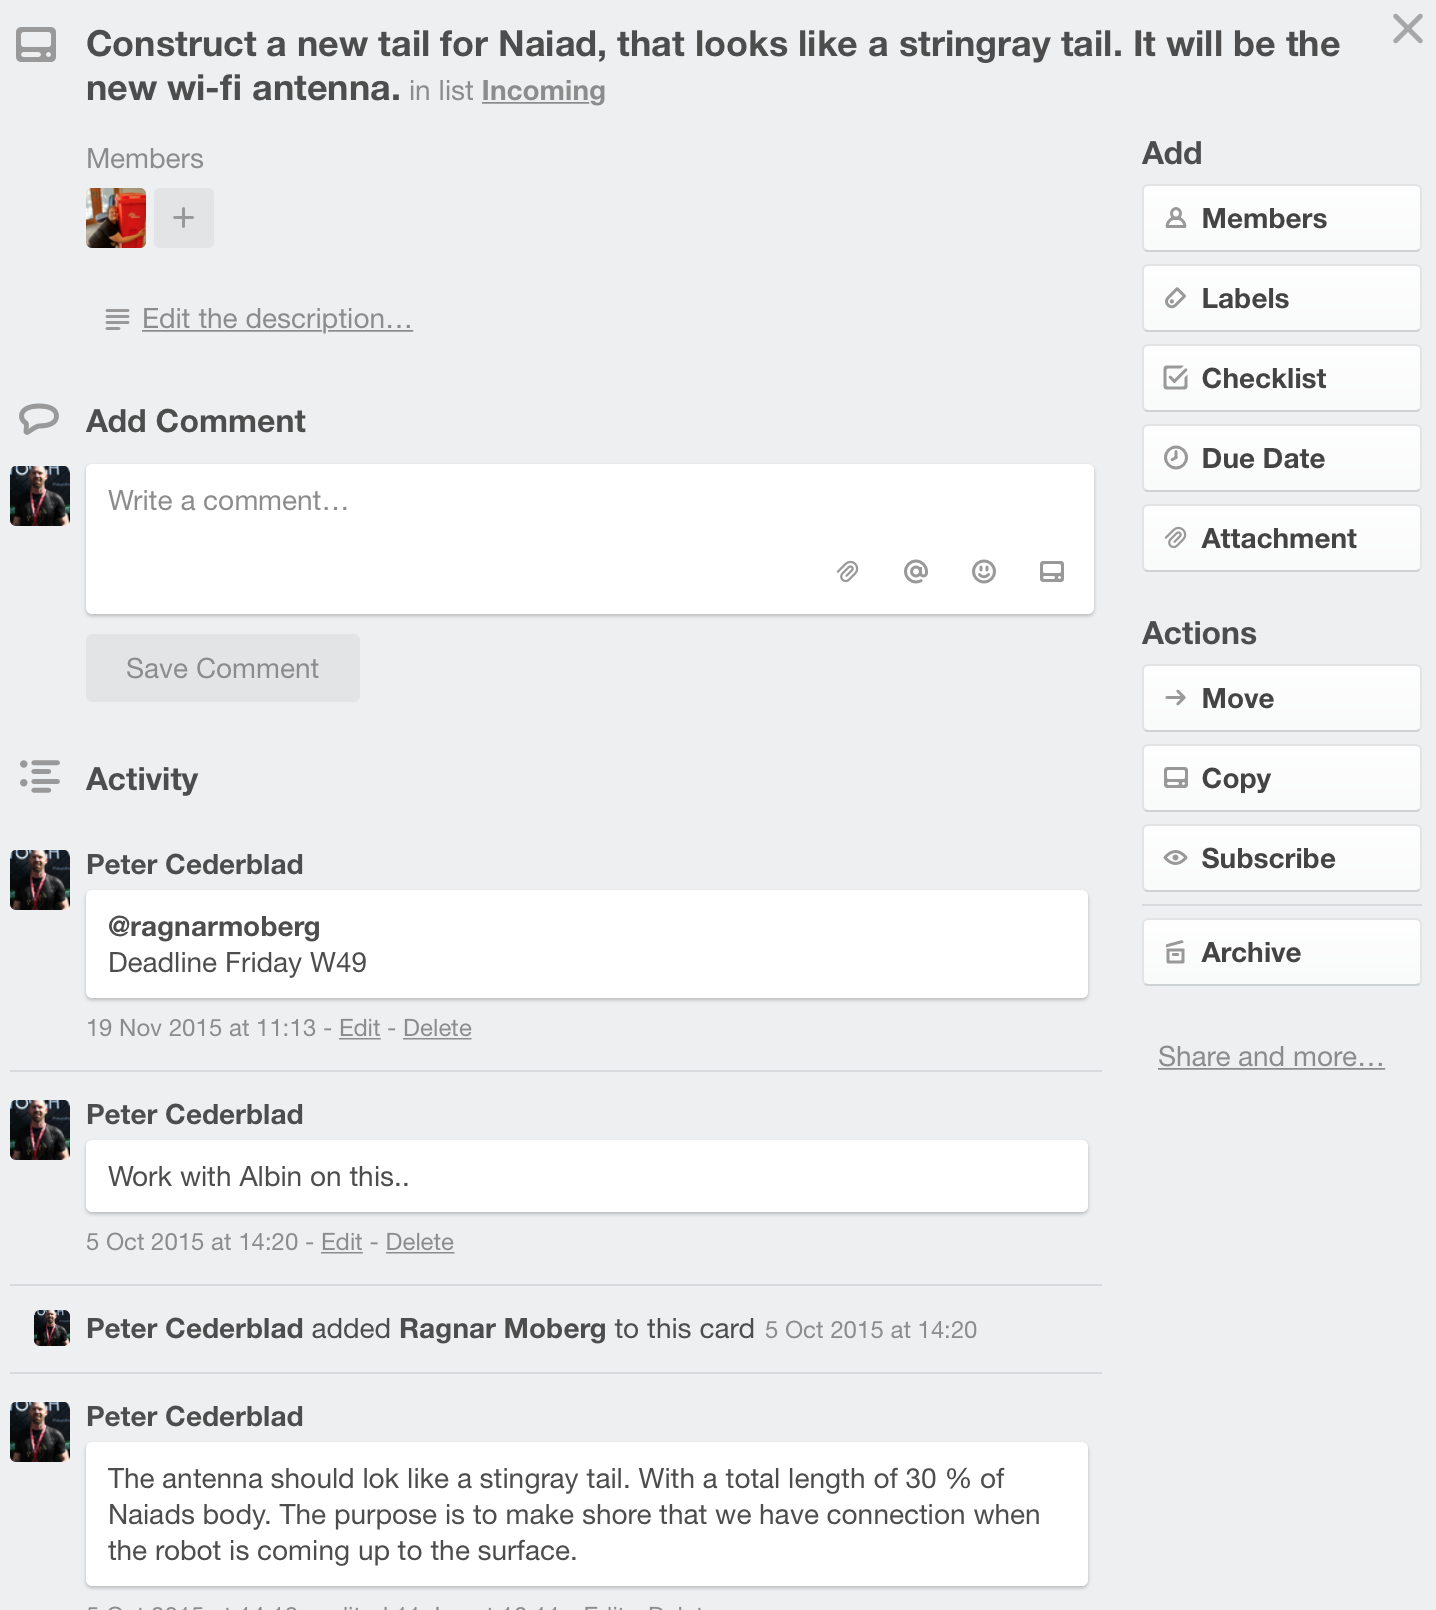
\includegraphics[scale=0.5]{Screenshoot28}

    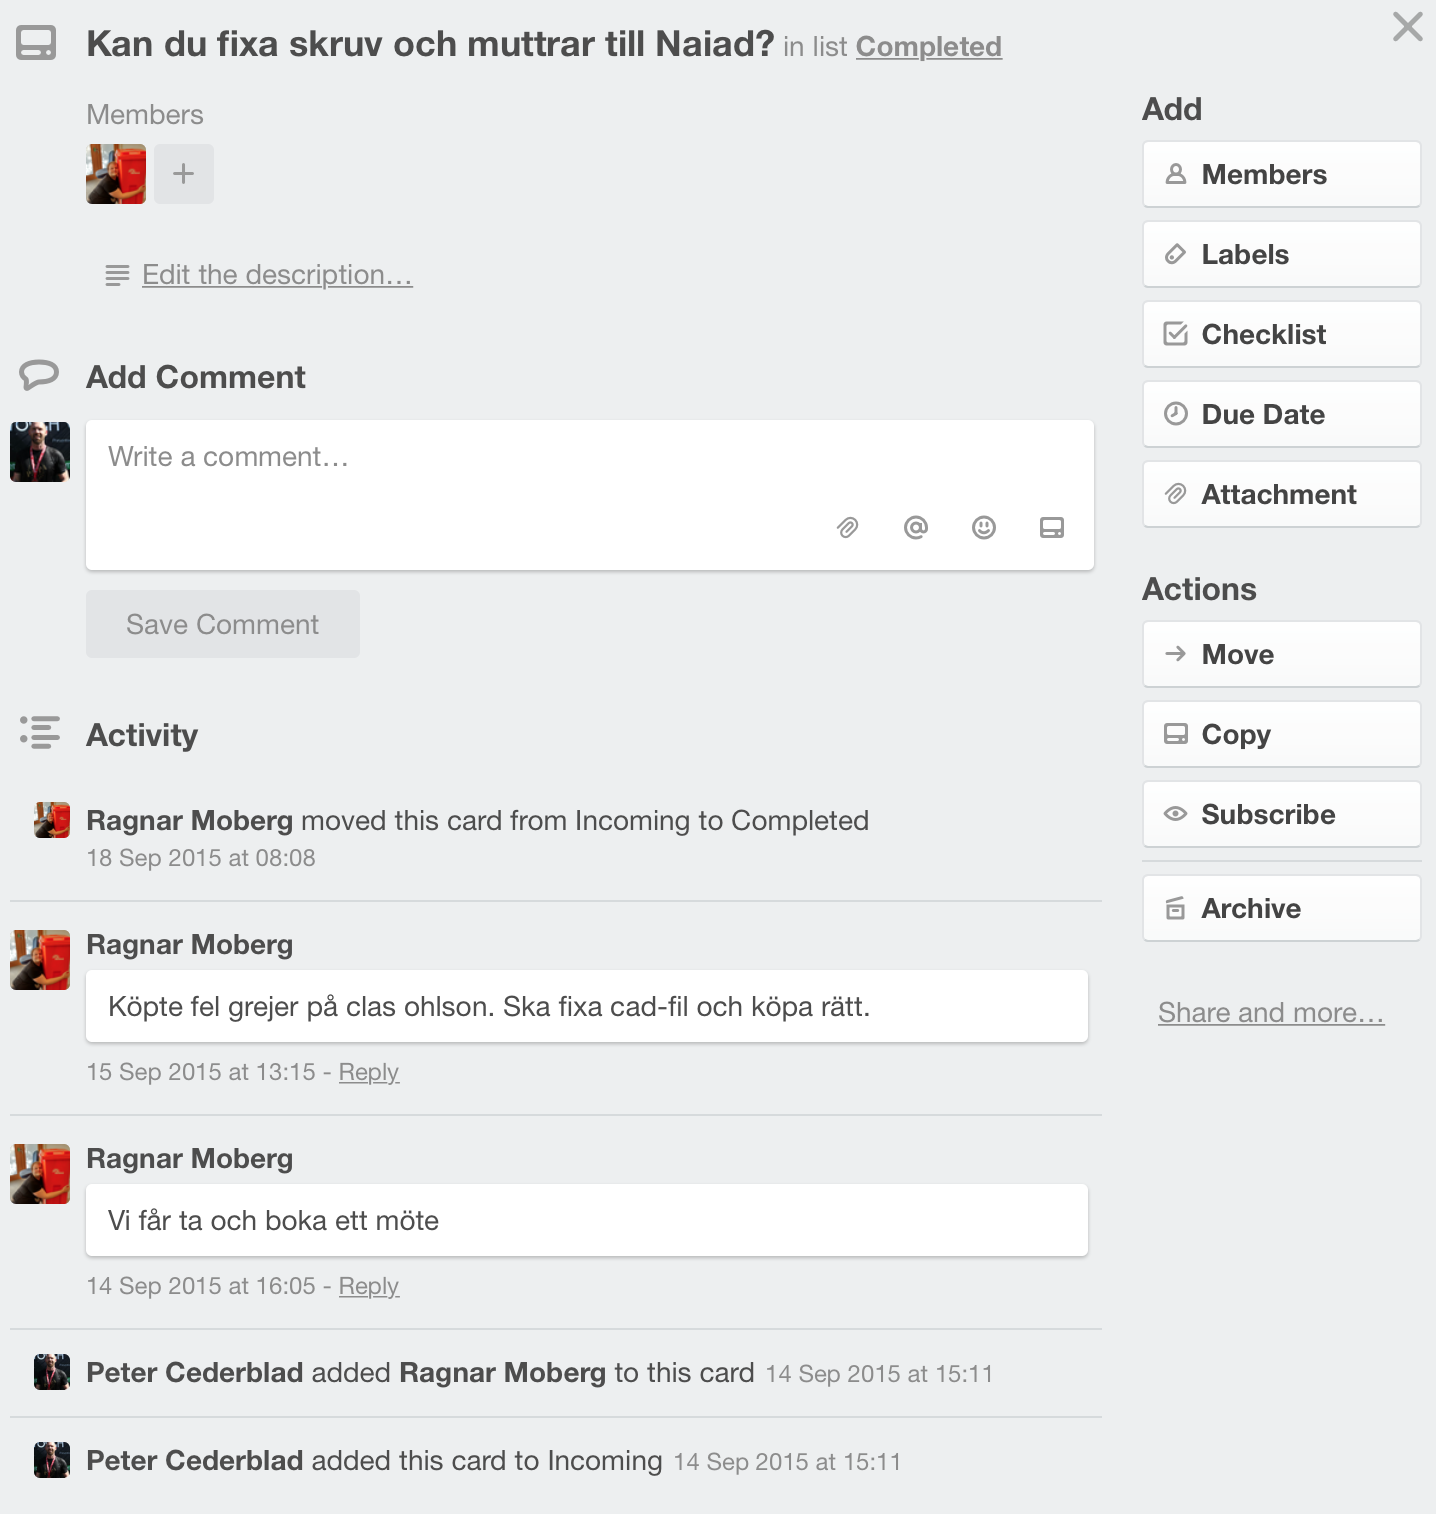
\includegraphics[scale=0.5]{Screenshoot29}


\newpage
\subsection{Software trello Cards}

    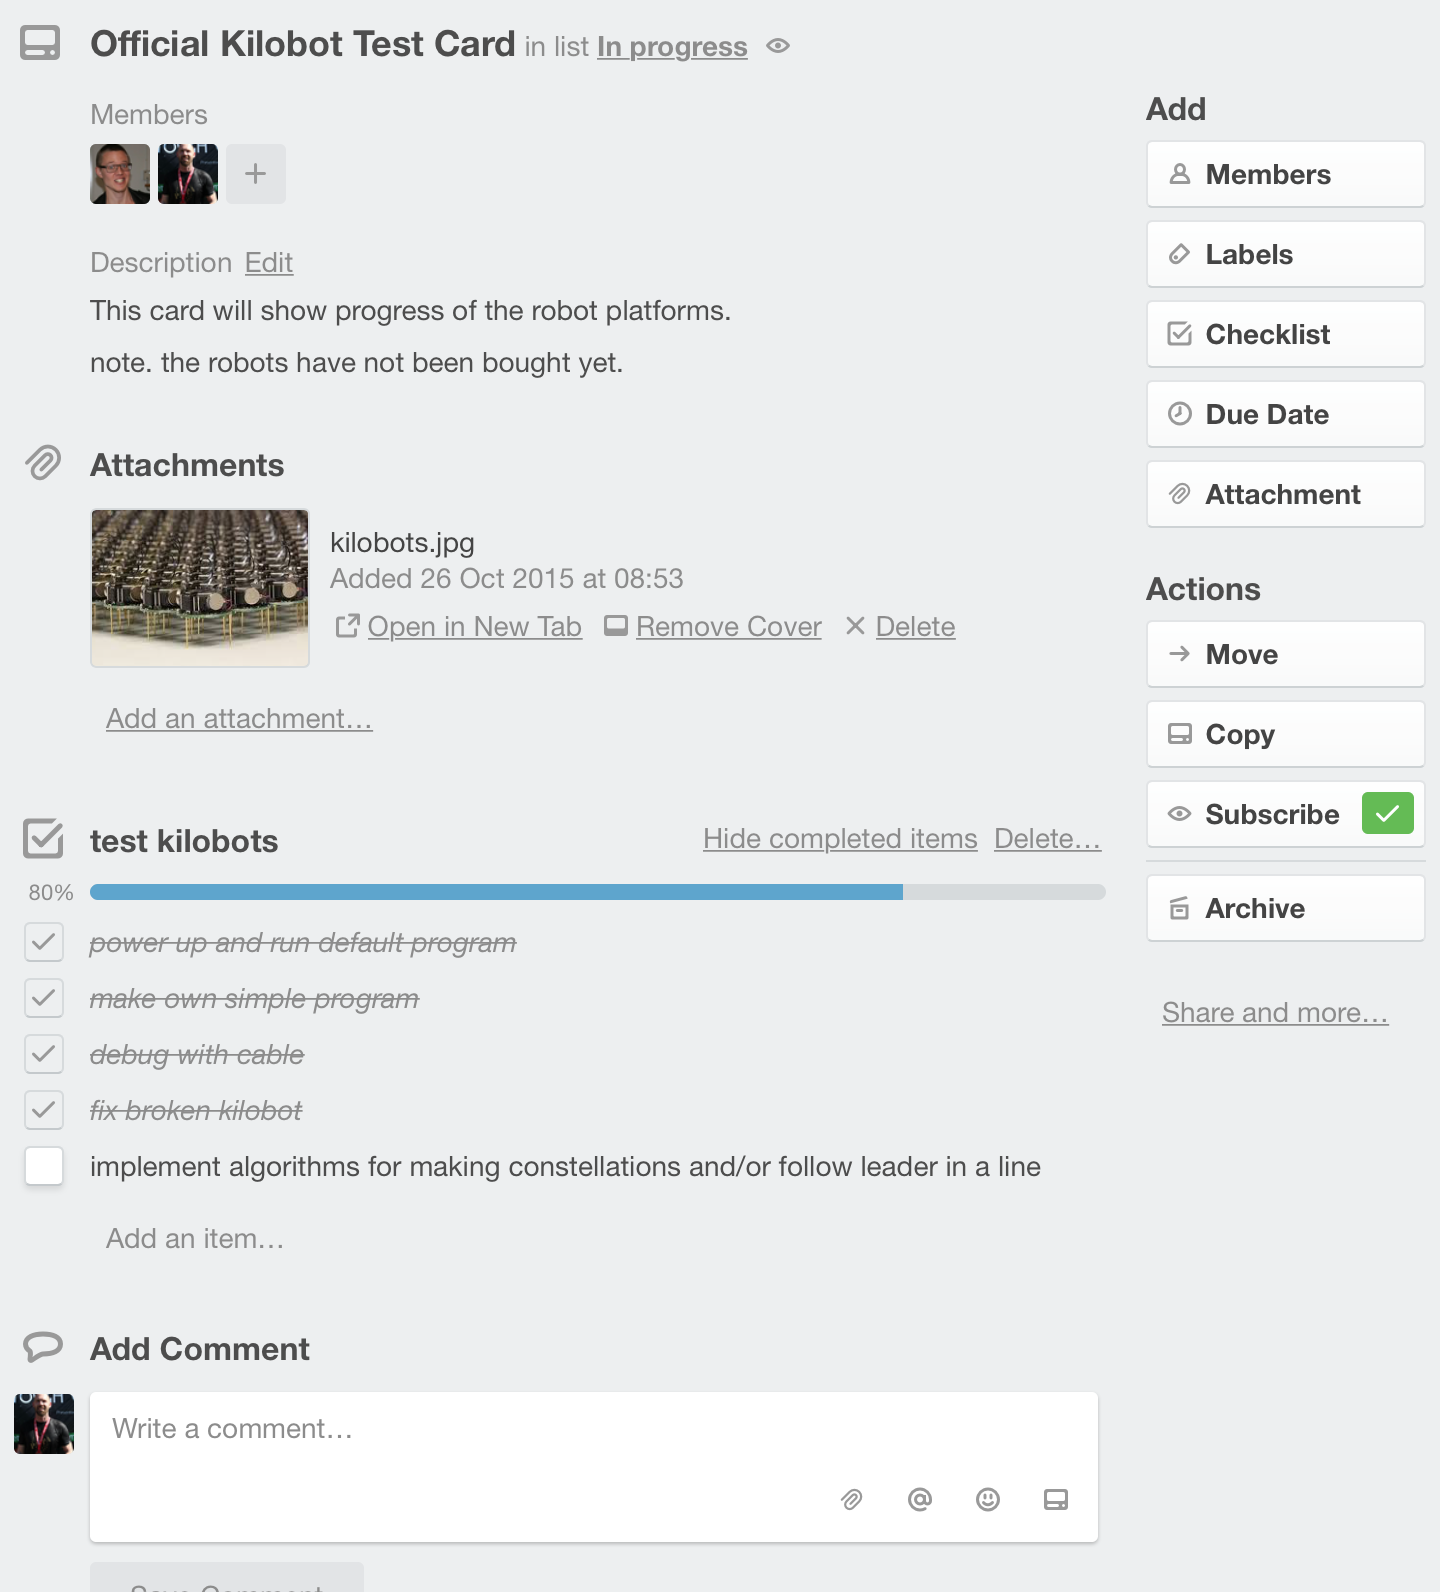
\includegraphics[scale=0.5]{Screenshoot30}

    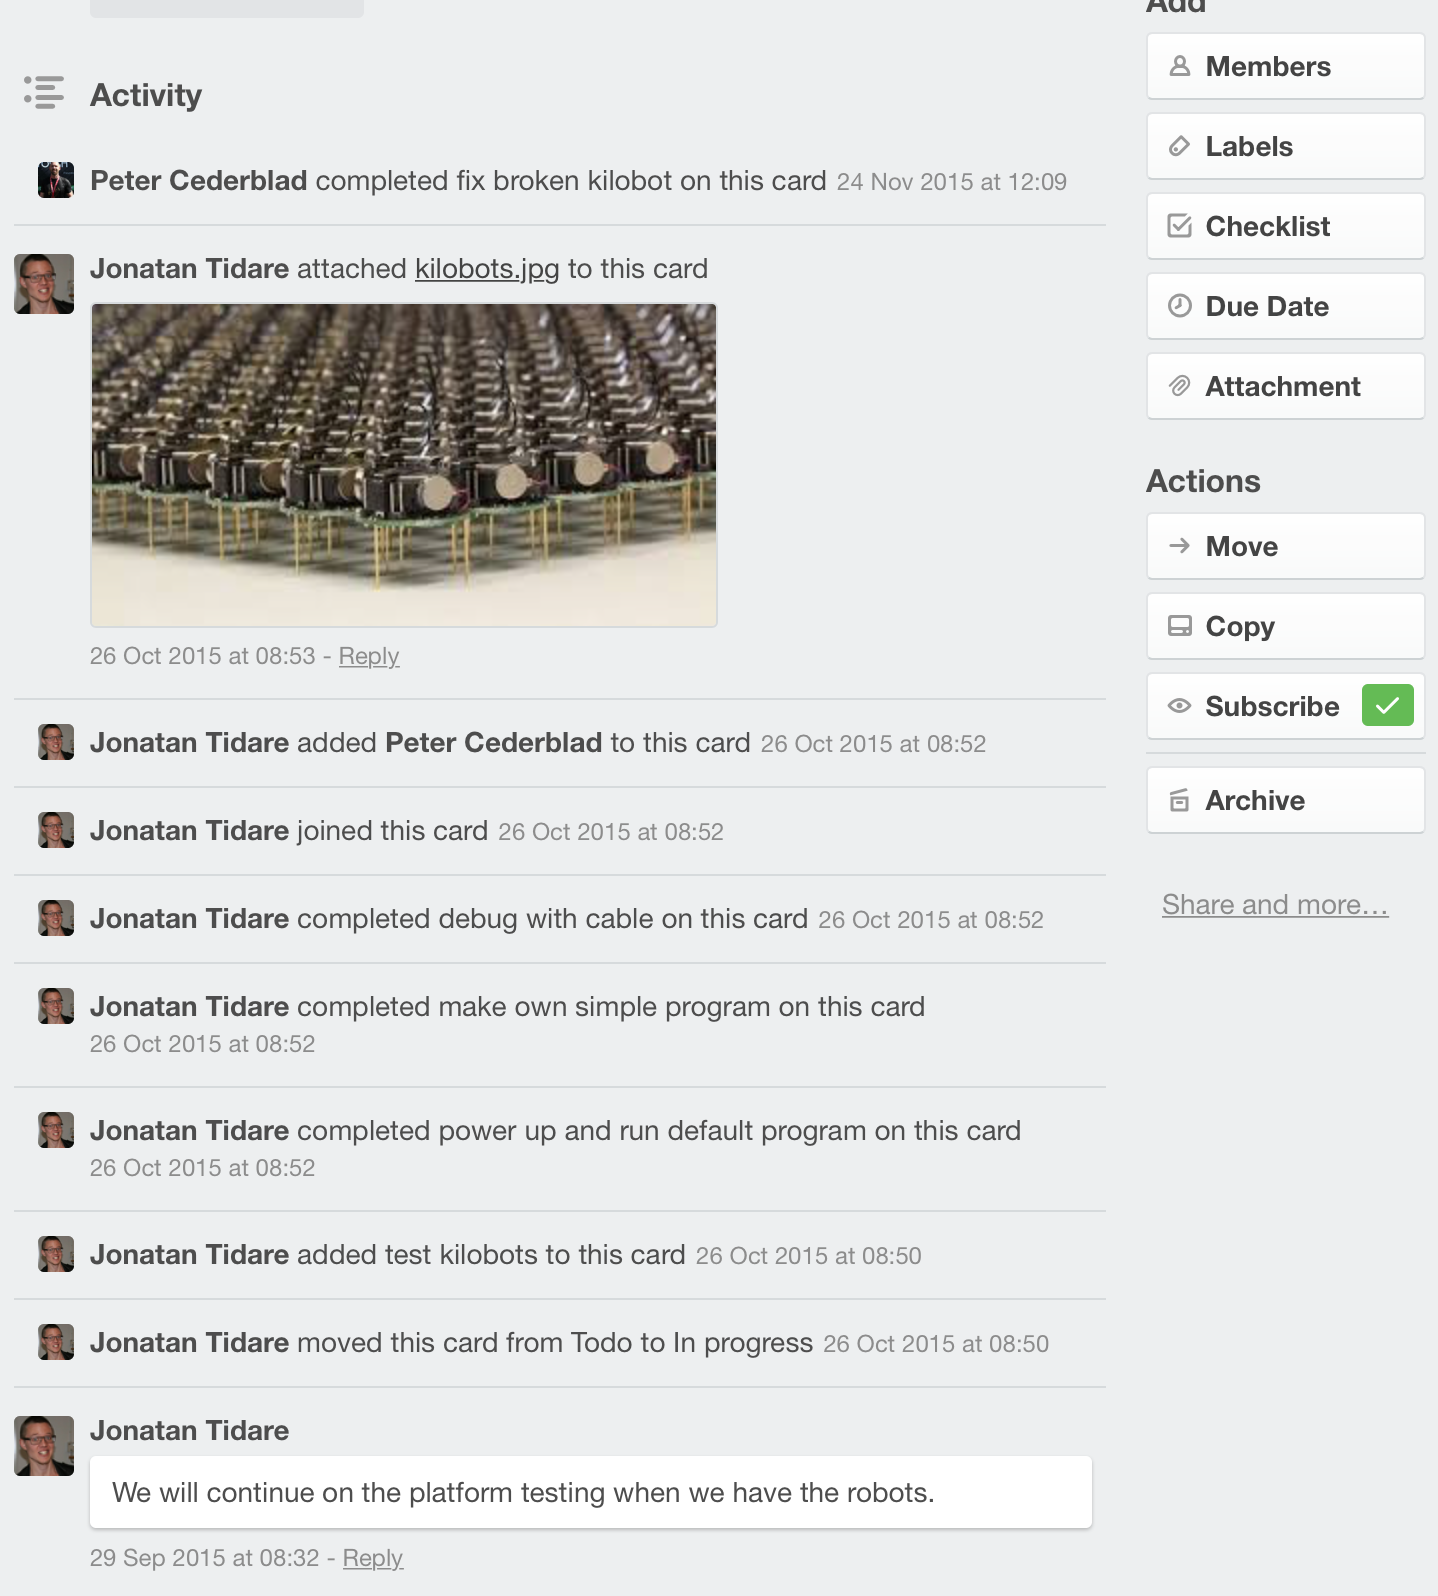
\includegraphics[scale=0.5]{Screenshoot31}

    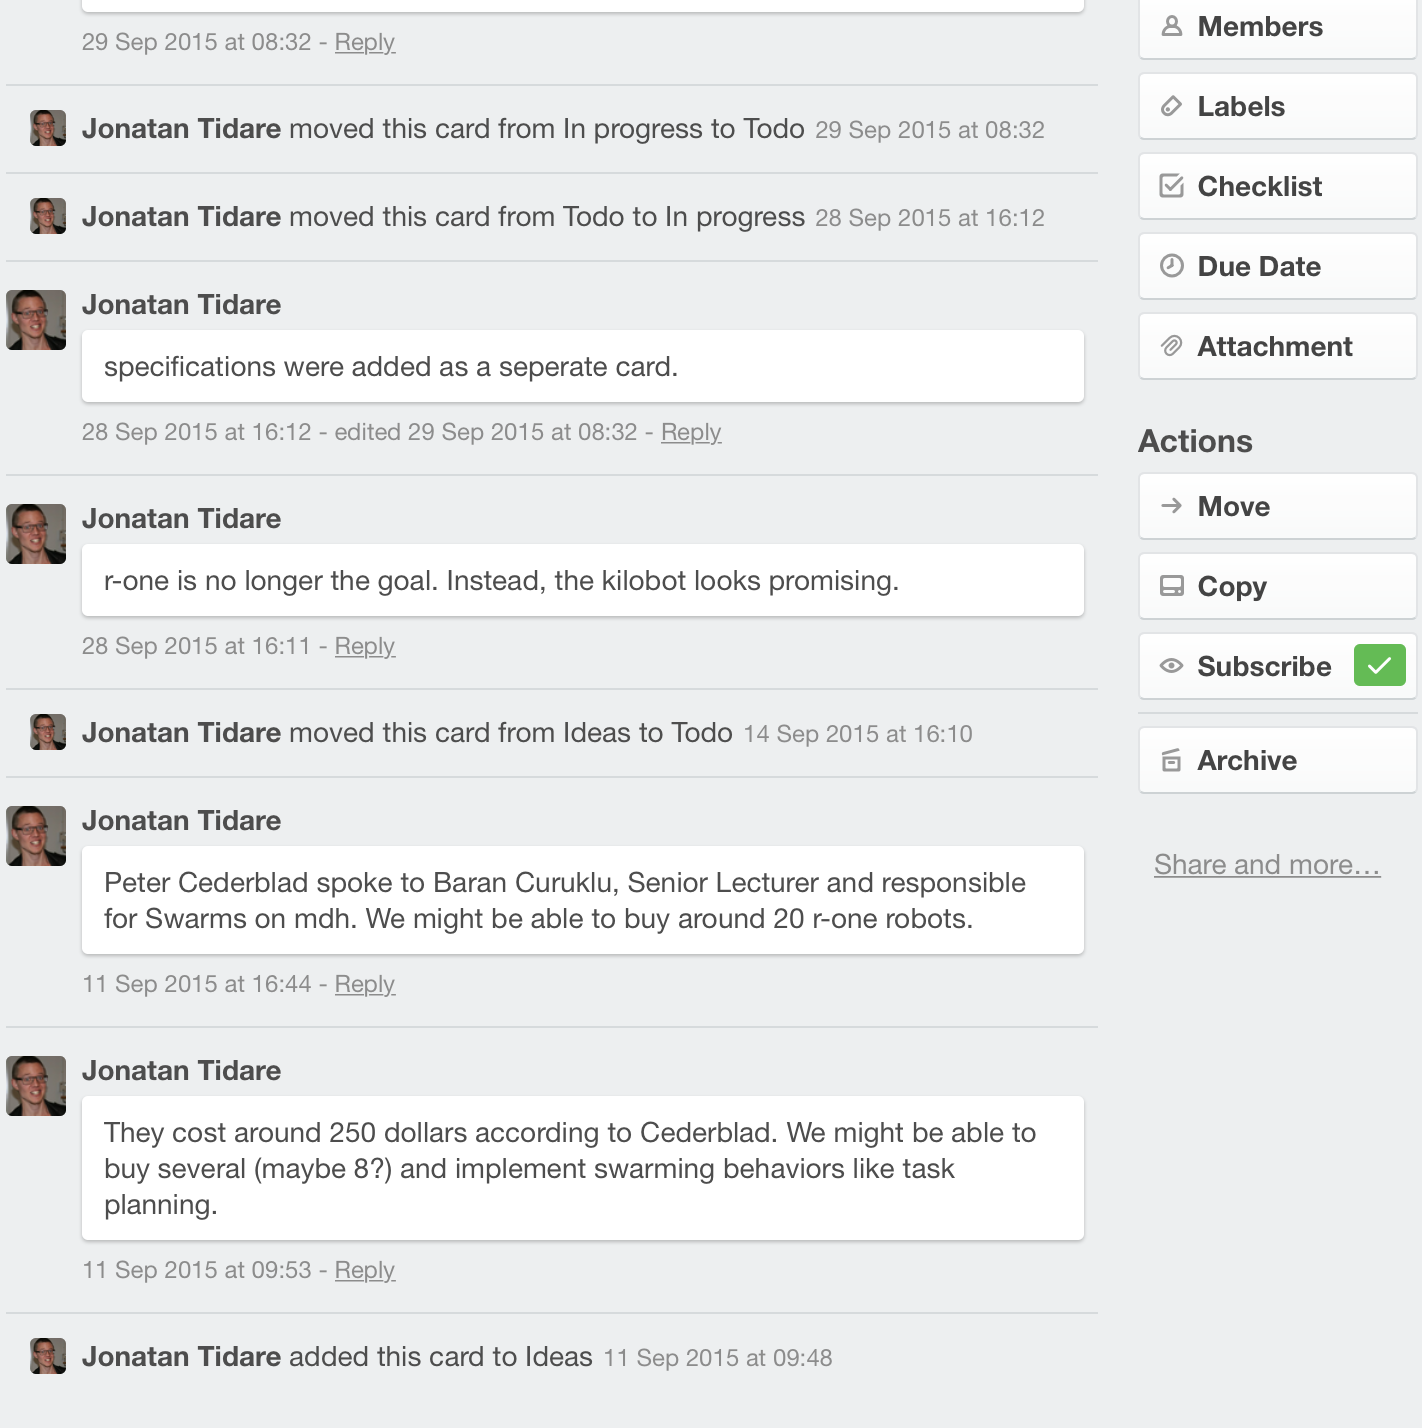
\includegraphics[scale=0.5]{Screenshoot32}

    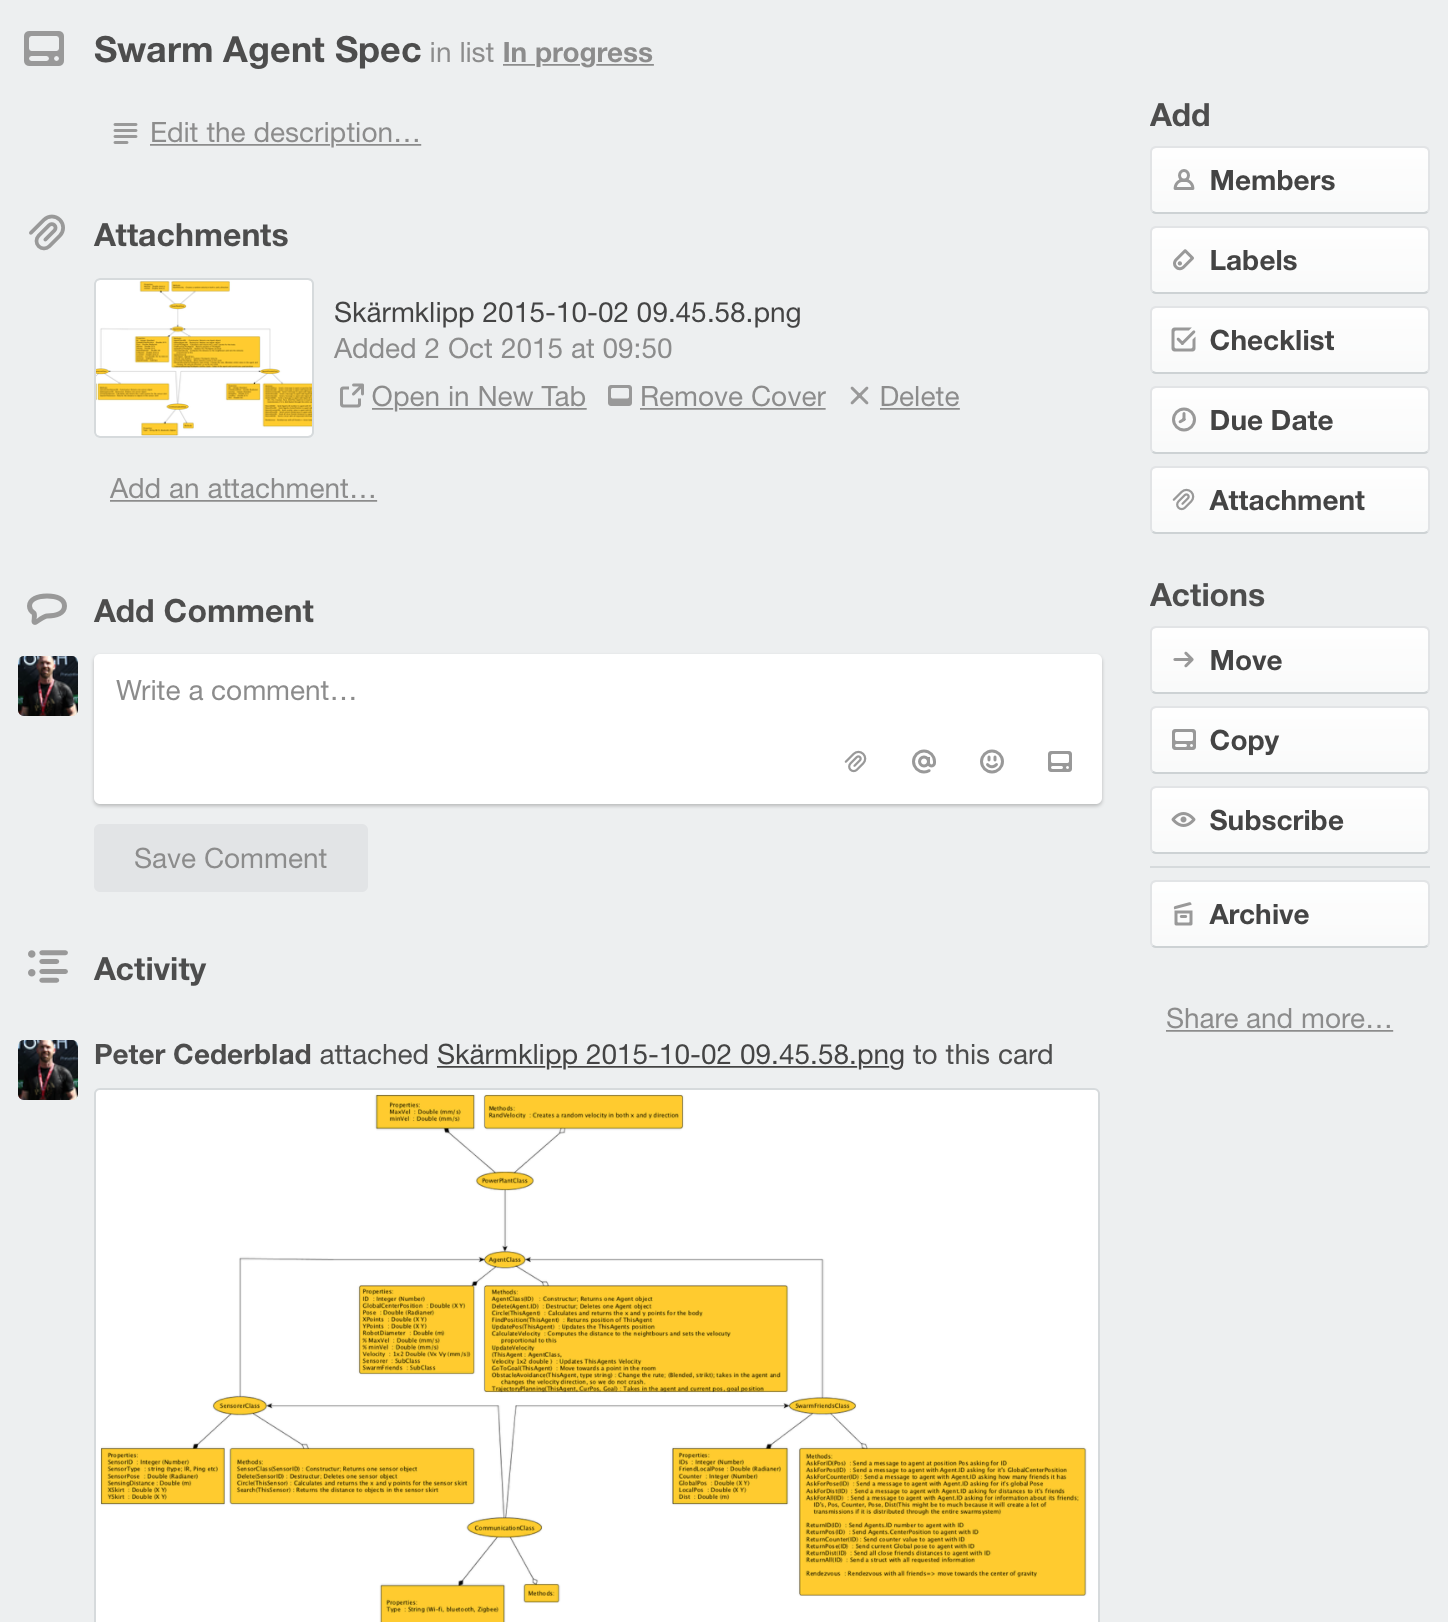
\includegraphics[scale=0.5]{Screenshoot33}

    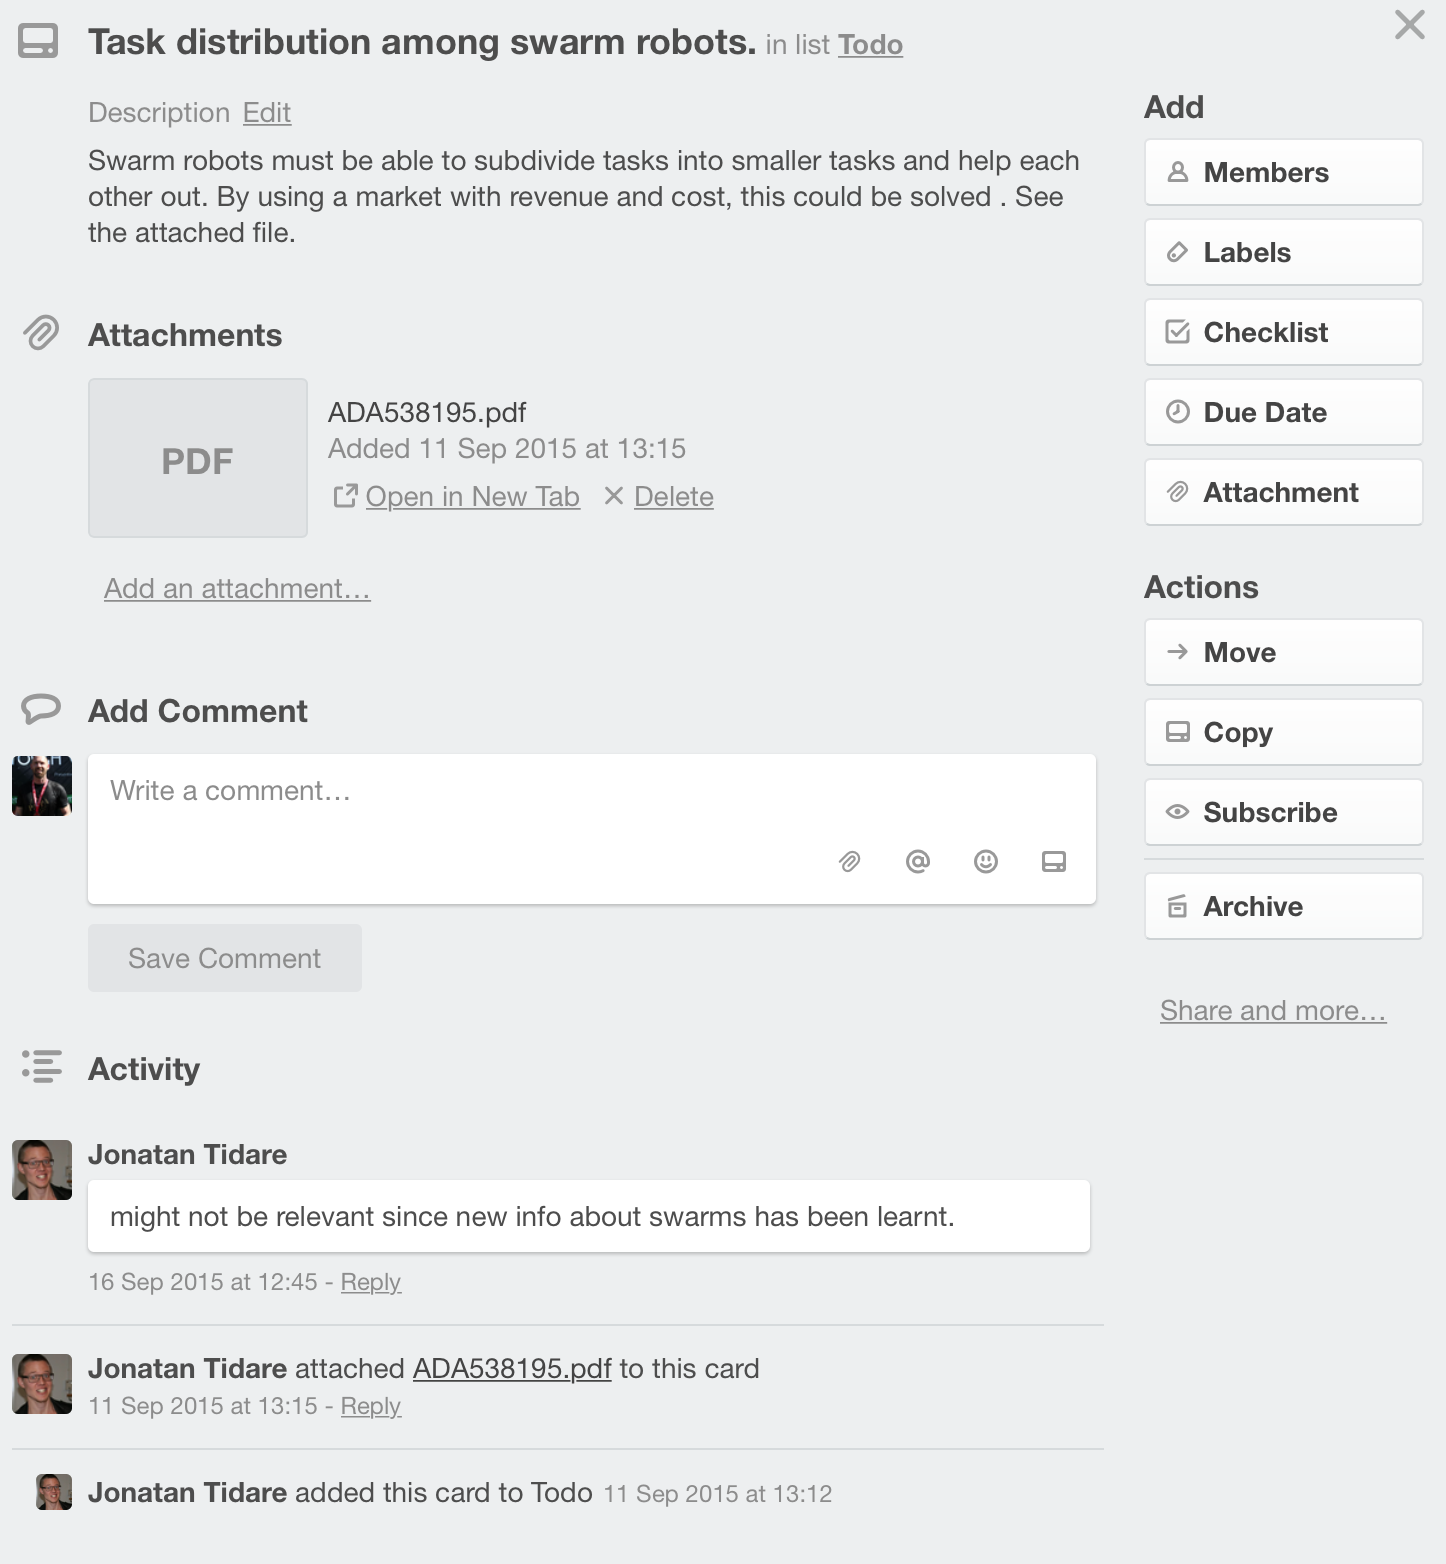
\includegraphics[scale=0.5]{Screenshoot34}

    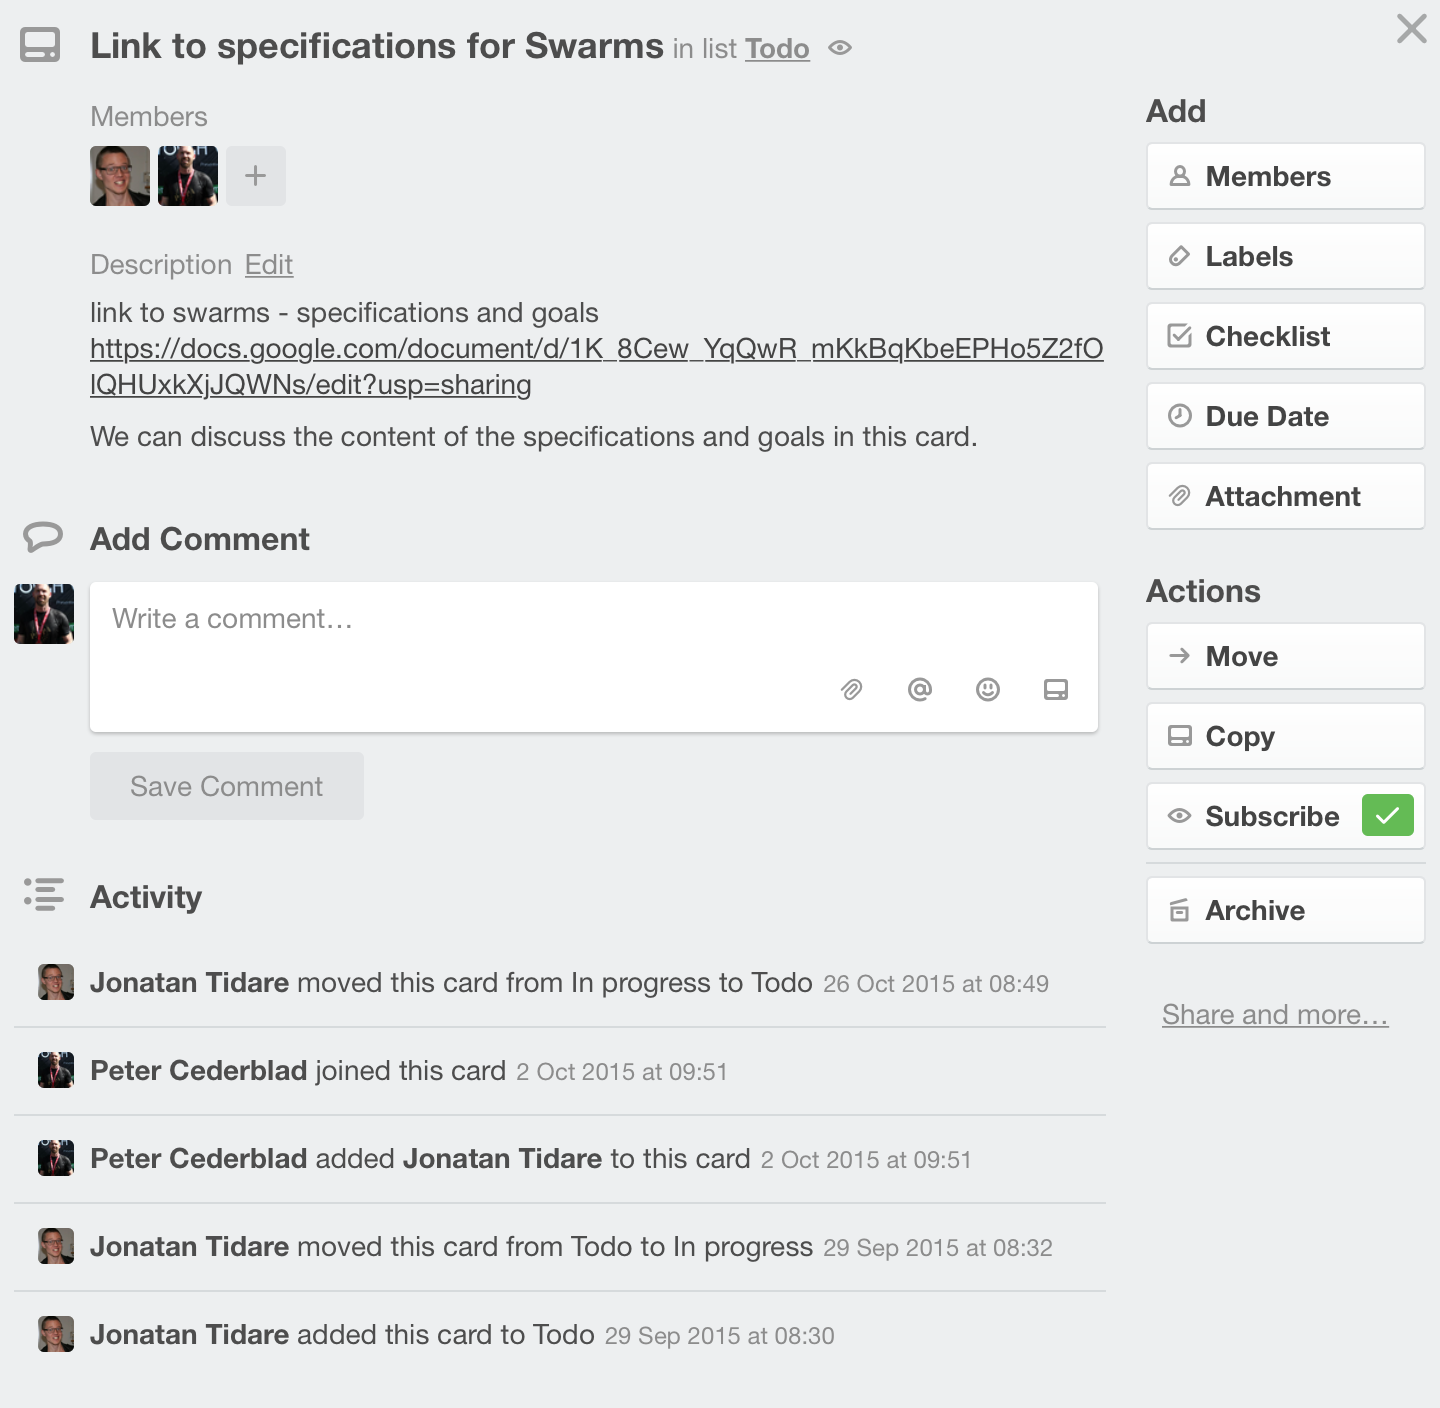
\includegraphics[scale=0.5]{Screenshoot35}

    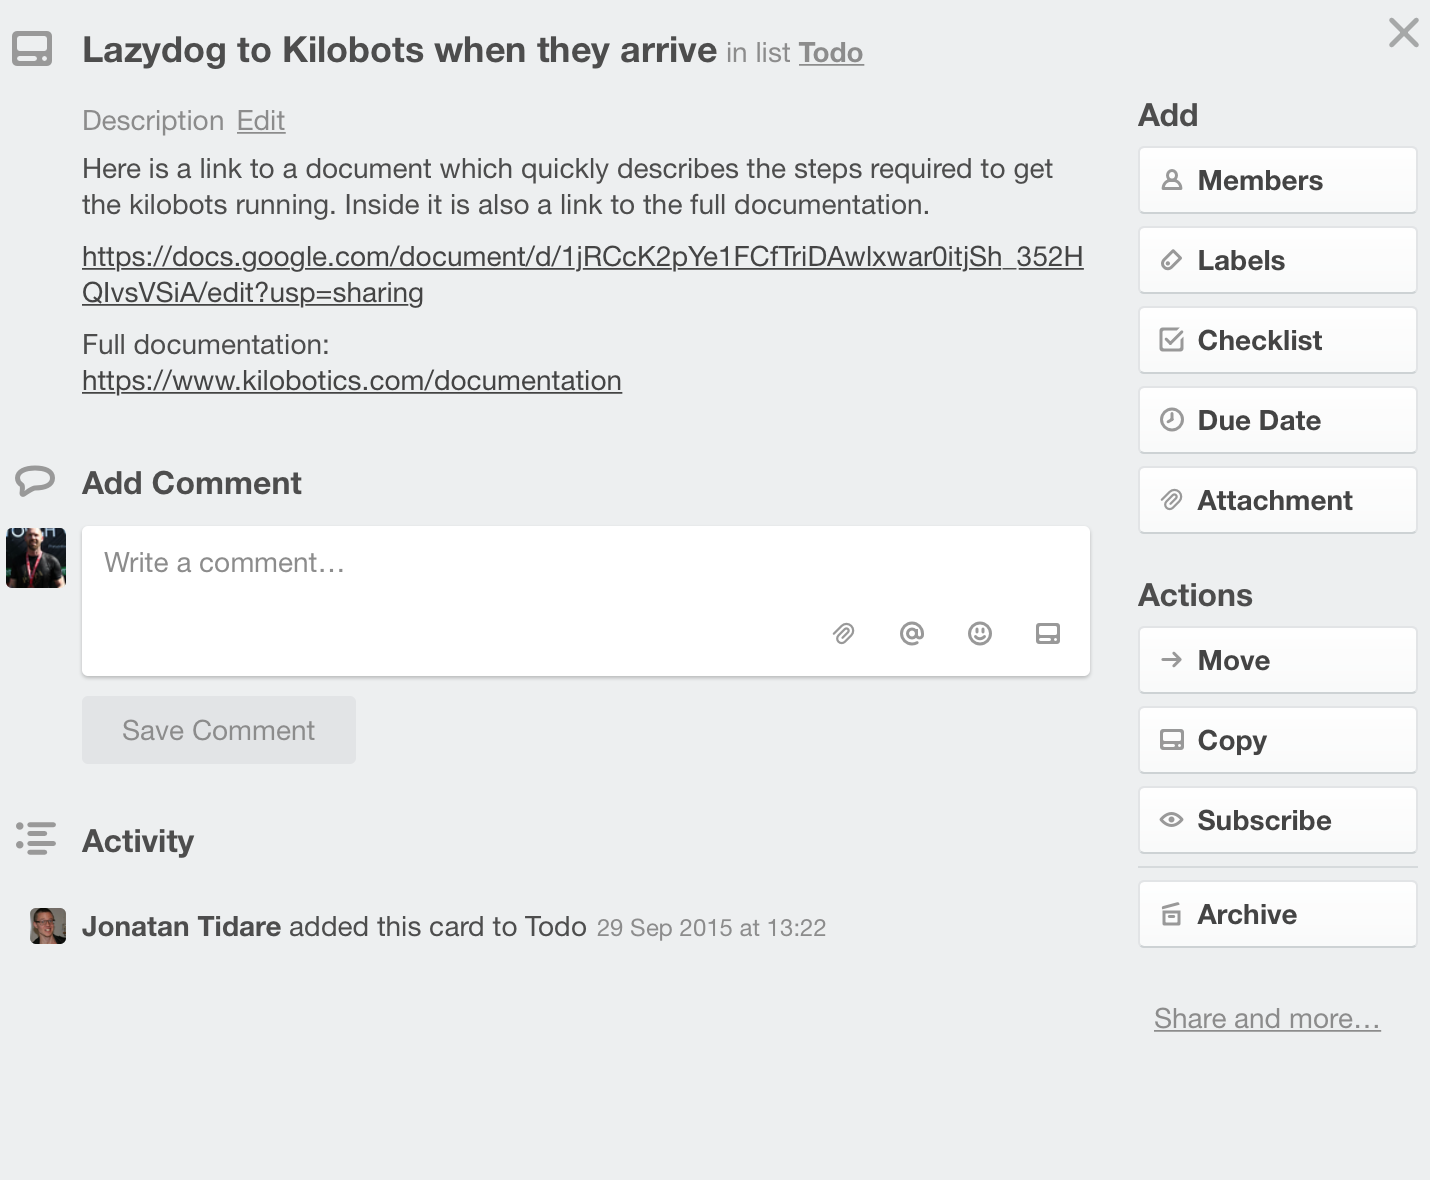
\includegraphics[scale=0.5]{Screenshoot36}

    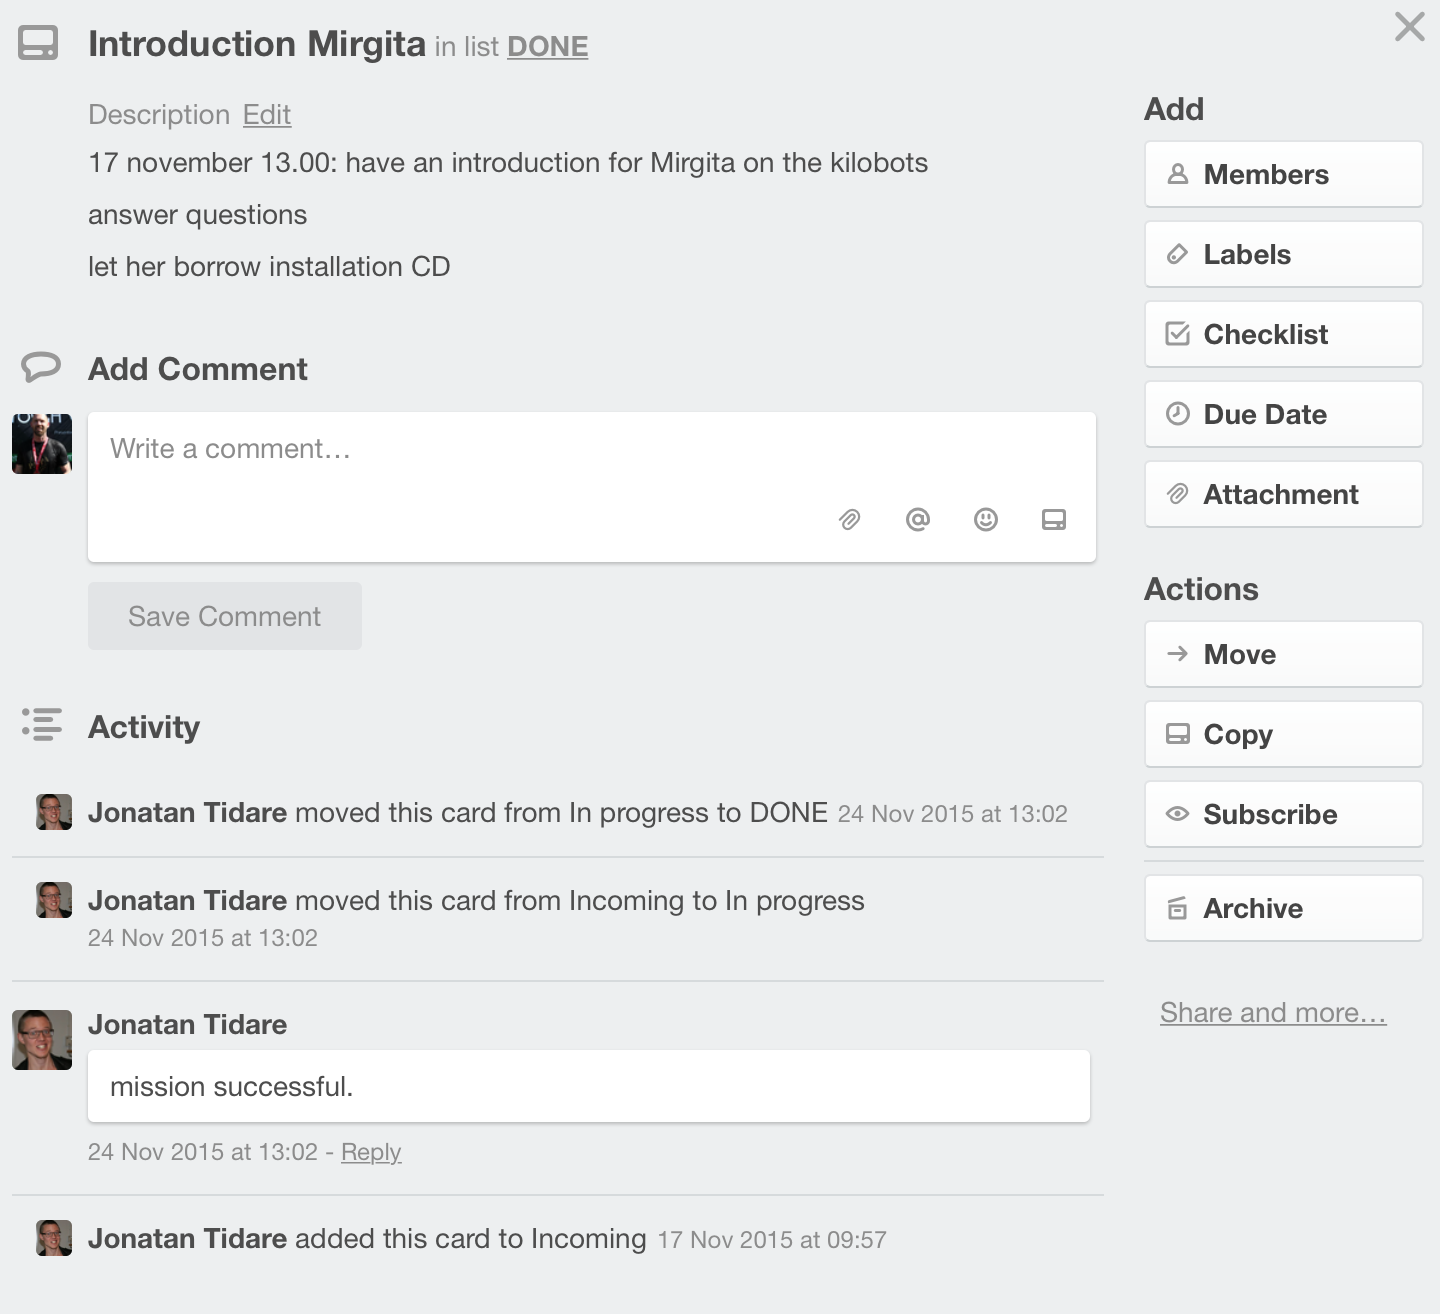
\includegraphics[scale=0.5]{Screenshoot37}


%%\subsection{Comunication trello Cards}
%
\subsection{Comunication trello Cards}

    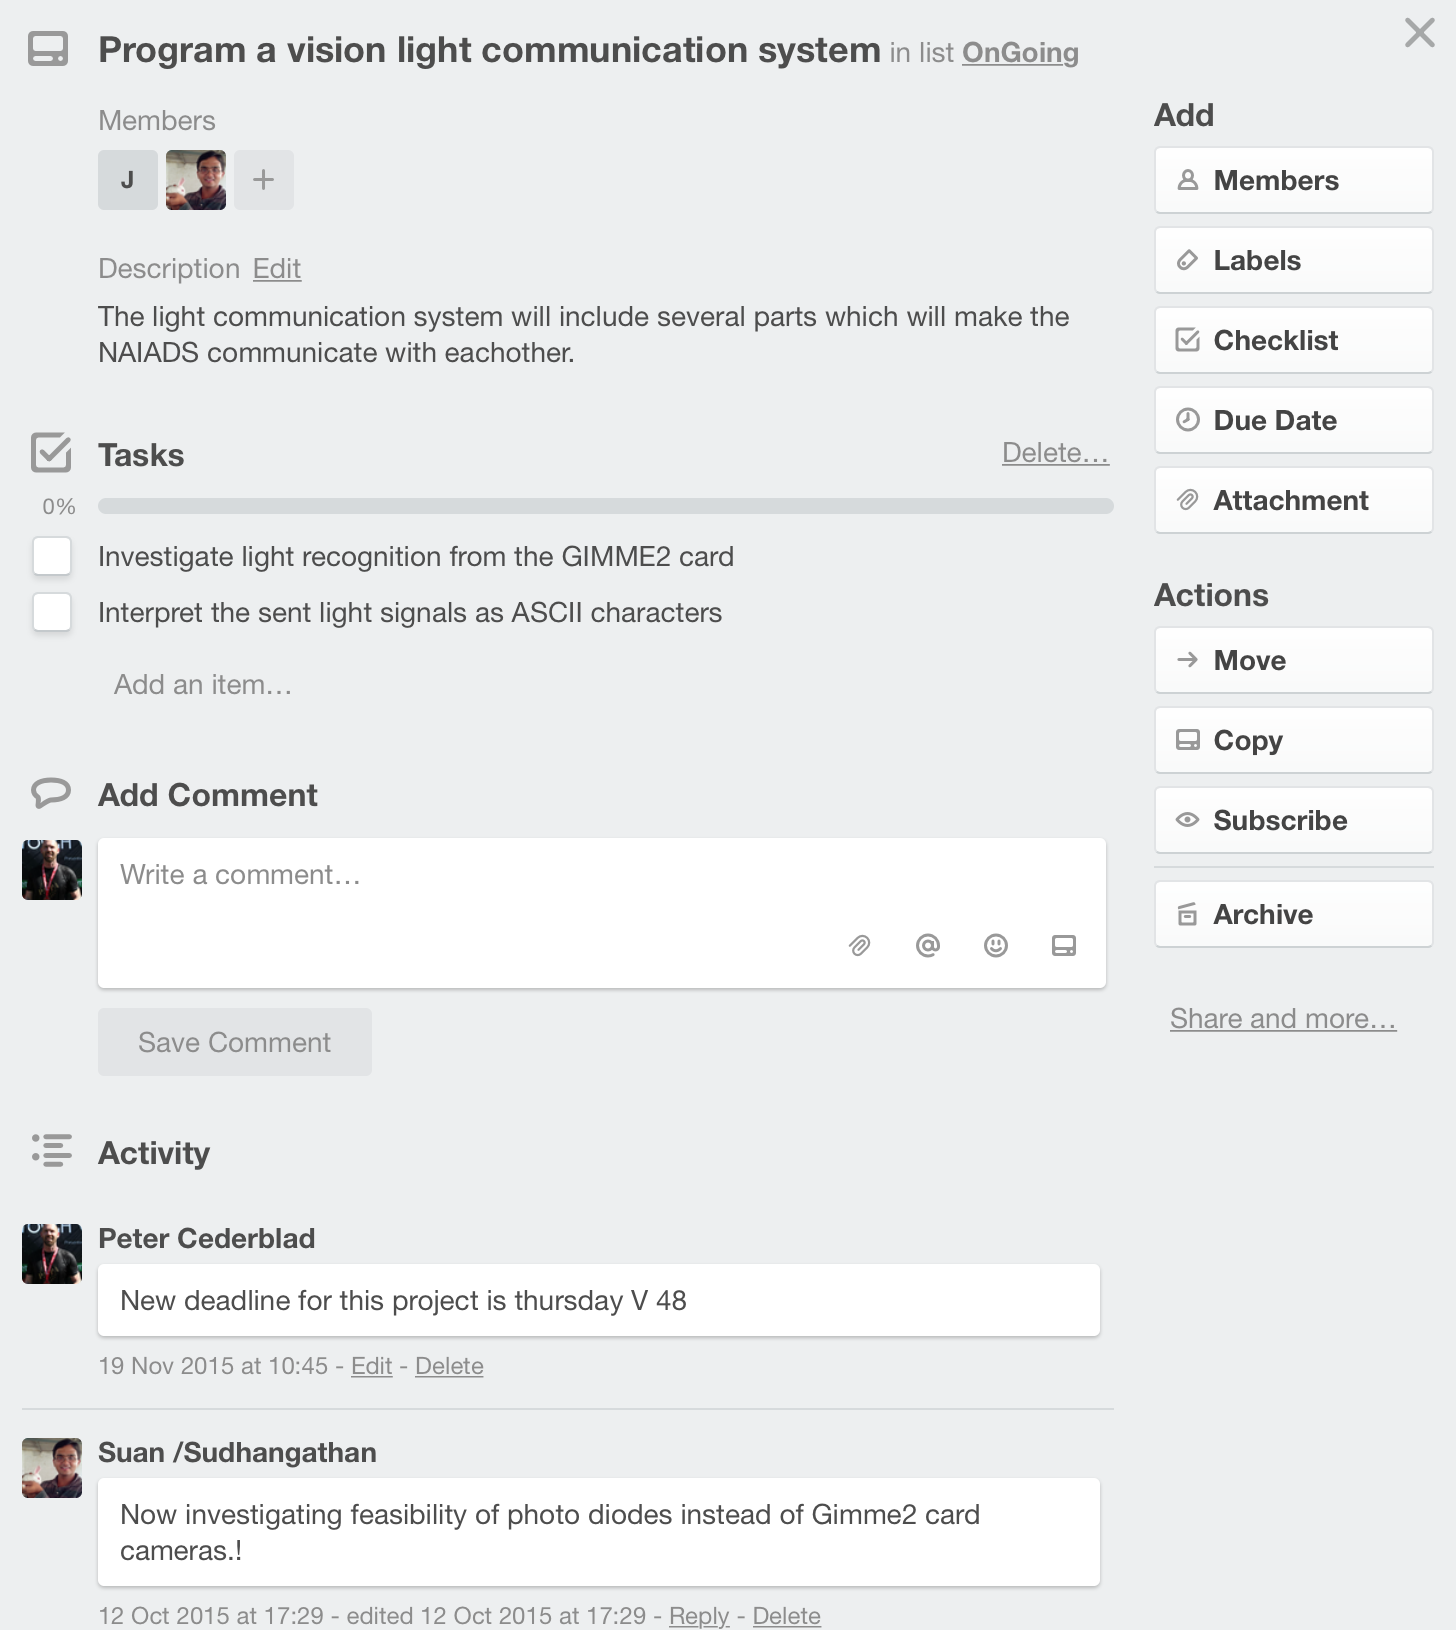
\includegraphics[scale=0.5]{Screenshoot1}

    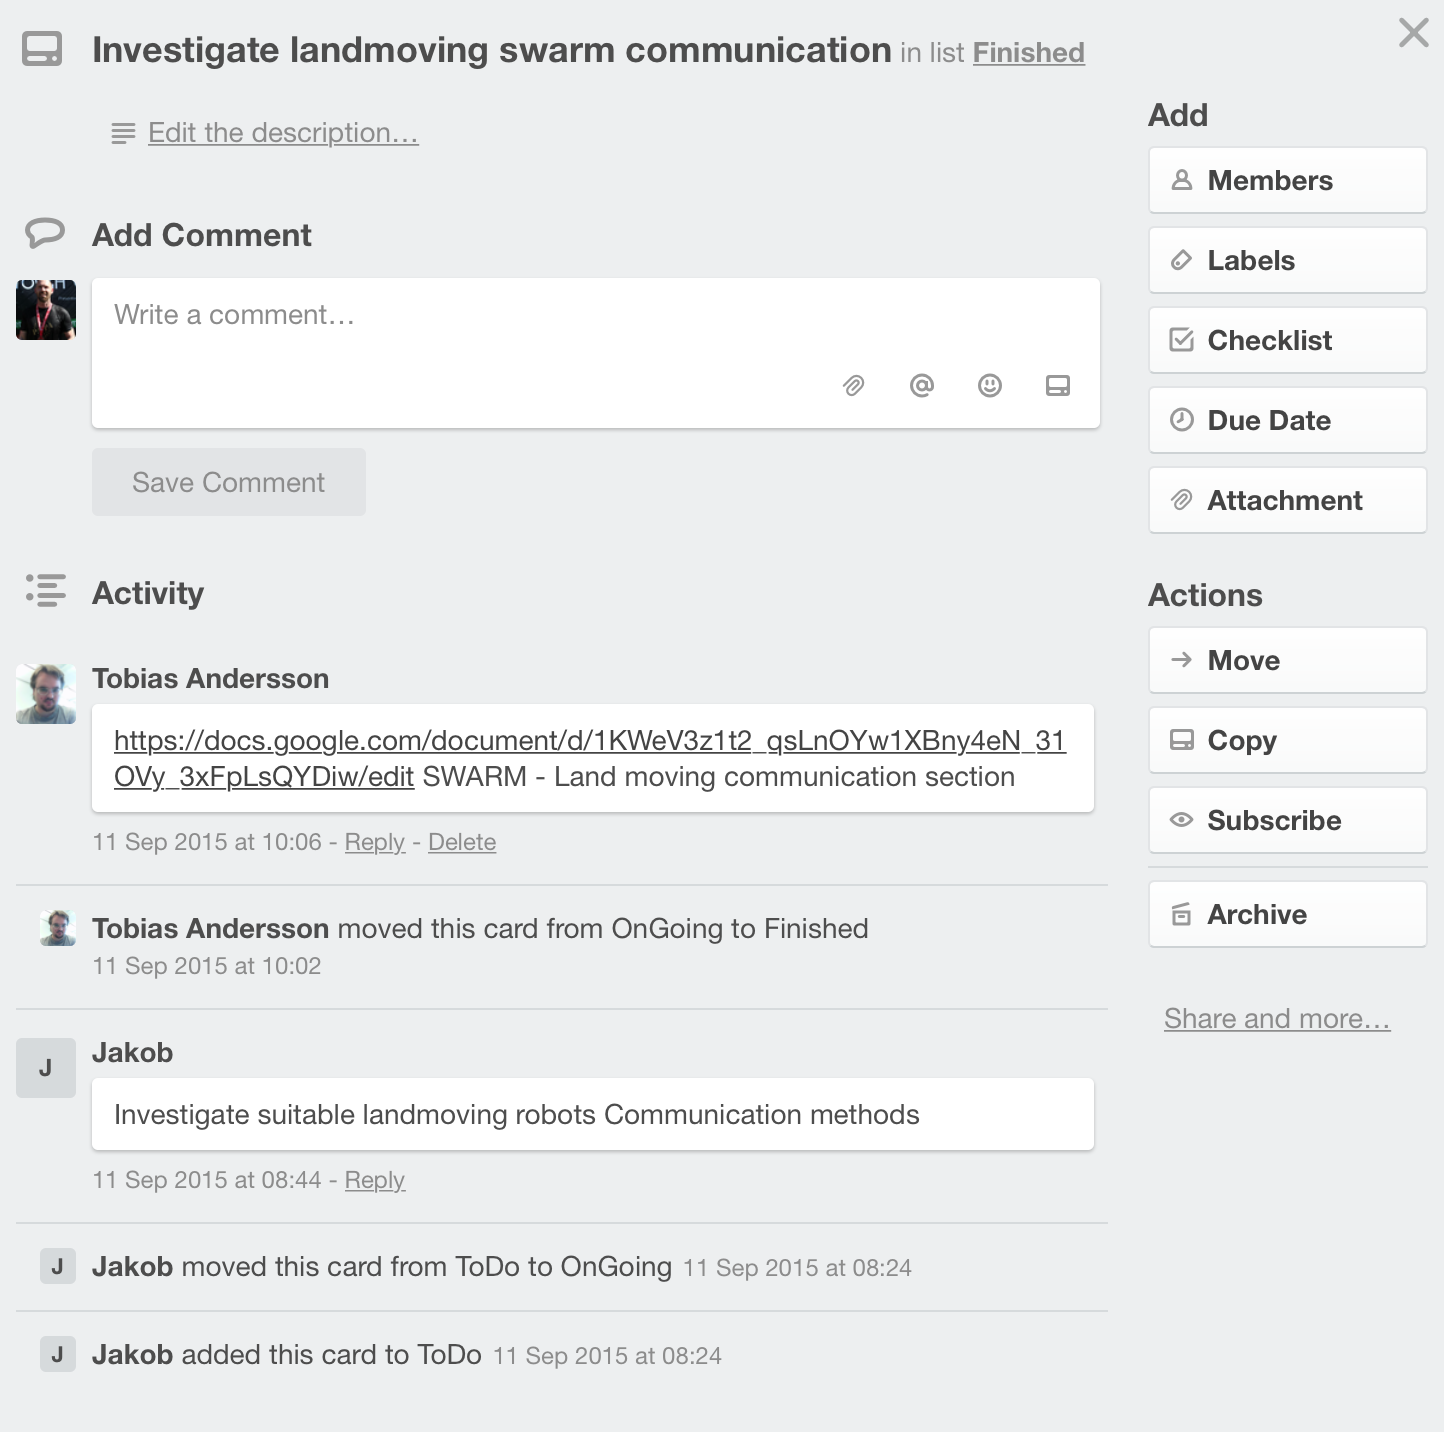
\includegraphics[scale=0.5]{Screenshoot2}
    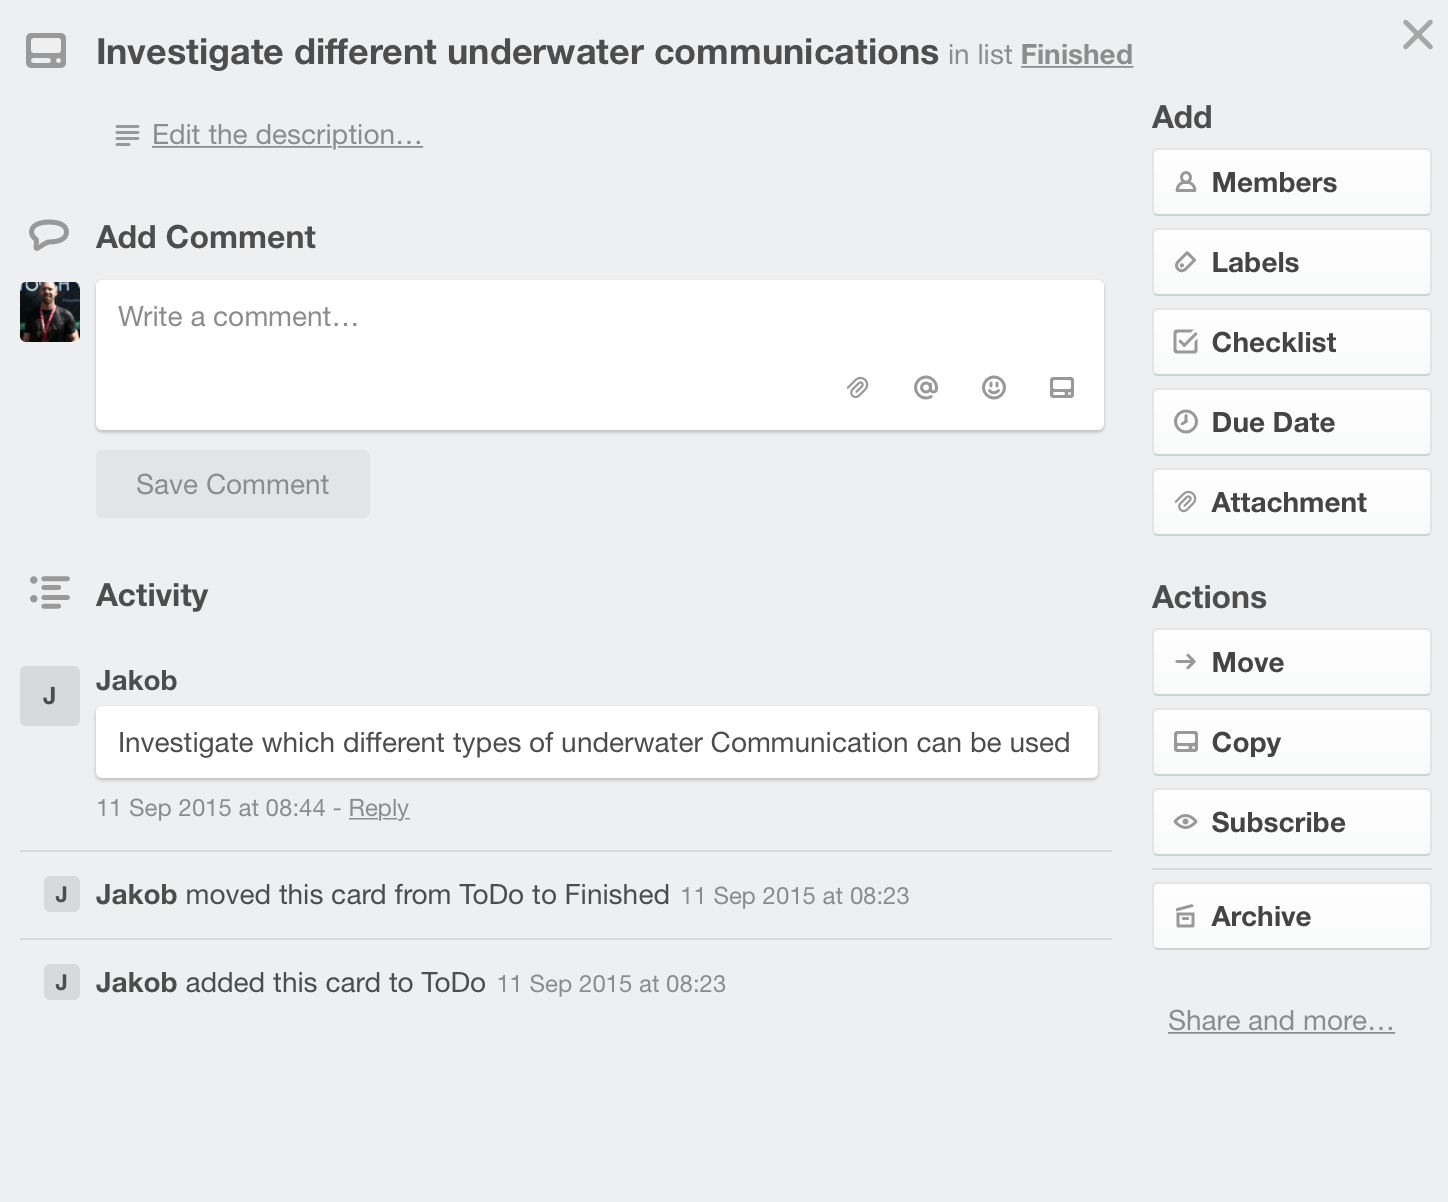
\includegraphics[scale=0.5]{Screenshoot3}

    \includegraphics[scale=0.5]{Screenshoot4}

%%\begin{figure}[!htbp]
%%\centering  
%%    \includegraphics[scale=0.5]{Screenshoot1}
%%\end{figure}
%%
%%
%%\begin{figure}[!htbp]
%%\centering  
%%    \includegraphics[scale=0.5]{Screenshoot2}
%%\end{figure}
%%
%%
%%\begin{figure}[!htbp]
%%\centering  
%%    \includegraphics[scale=0.5]{Screenshoot3}
%%\end{figure}
%%
%%
%%\begin{figure}[!htbp]
%%\centering  
%%    \includegraphics[scale=0.5]{Screenshoot4}
%%\end{figure}
%
%
%
%
%
%\newpage
%\subsection{Hardware trello Cards}
%\begin{figure}[!htbp]
%\centering  
%    \includegraphics[scale=0.5]{Screenshoot5}
%\end{figure}
%
%
%\begin{figure}[h]
%\centering  
%    \includegraphics[scale=0.5]{Screenshoot6}
%\end{figure}
%
%
%\begin{figure}[h]
%\centering  
%    \includegraphics[scale=0.5]{Screenshoot7}
%\end{figure}
%
%
%\begin{figure}[]
%\centering  
%    \includegraphics[scale=0.5]{Screenshoot8}
%\end{figure}
%
%
%\begin{figure}[h]
%\centering  
%    \includegraphics[scale=0.5]{Screenshoot9}
%\end{figure}
%
%
%\begin{figure}[h]
%\centering  
%    \includegraphics[scale=0.5]{Screenshoot10}
%\end{figure}
%
%
%\begin{figure}[h]
%\centering  
%    \includegraphics[scale=0.5]{Screenshoot11}
%\end{figure}
%
%
%\begin{figure}[h]
%\centering  
%    \includegraphics[scale=0.5]{Screenshoot12}
%\end{figure}
%
%
%\begin{figure}[h]
%\centering  
%    \includegraphics[scale=0.5]{Screenshoot13}
%\end{figure}
%
%
%\begin{figure}[h]
%\centering  
%    \includegraphics[scale=0.5]{Screenshoot14}
%\end{figure}
%
%
%\begin{figure}[h]
%\centering  
%    \includegraphics[scale=0.5]{Screenshoot15}
%\end{figure}
%
%
%\begin{figure}[h]
%\centering  
%    \includegraphics[scale=0.5]{Screenshoot16}
%\end{figure}
%
%
%\begin{figure}[h]
%\centering  
%    \includegraphics[scale=0.5]{Screenshoot17}
%\end{figure}
%
%
%\begin{figure}[h]
%\centering  
%    \includegraphics[scale=0.5]{Screenshoot18}
%\end{figure}
%
%
%\begin{figure}[h]
%\centering  
%    \includegraphics[scale=0.5]{Screenshoot19}
%\end{figure}
%
%
%\begin{figure}[h]
%\centering  
%    \includegraphics[scale=0.5]{Screenshoot20}
%\end{figure}
%
%
%\begin{figure}[h]
%\centering  
%    \includegraphics[scale=0.5]{Screenshoot21}
%\end{figure}
%
%
%\begin{figure}[h]
%\centering  
%    \includegraphics[scale=0.5]{Screenshoot22}
%\end{figure}
%
%\newpage
%\begin{figure}[h]
%\centering  
%    \includegraphics[scale=0.5]{Screenshoot23}
%\end{figure}
%
%
%
%\newpage
%\subsection{Mechanics trello Cards}
%
%\begin{figure}[h]
%\centering  
%    \includegraphics[scale=0.5]{Screenshoot24}
%\end{figure}
%
%
%\begin{figure}[h]
%\centering  
%    \includegraphics[scale=0.5]{Screenshoot25}
%\end{figure}
%
%
%\begin{figure}[h]
%\centering  
%    \includegraphics[scale=0.5]{Screenshoot26}
%\end{figure}
%
%
%\begin{figure}[h]
%\centering  
%    \includegraphics[scale=0.5]{Screenshoot27}
%\end{figure}
%
%
%\begin{figure}[h]
%\centering  
%    \includegraphics[scale=0.5]{Screenshoot28}
%\end{figure}
%
%
%\begin{figure}[h]
%\centering  
%    \includegraphics[scale=0.5]{Screenshoot29}
%\end{figure}
%
%
%
%\newpage
%\subsection{Software trello Cards}
%\begin{figure}[h]
%\centering  
%    \includegraphics[scale=0.5]{Screenshoot30}
%\end{figure}
%
%
%\begin{figure}[h]
%\centering  
%    \includegraphics[scale=0.5]{Screenshoot31}
%\end{figure}
%
%
%\begin{figure}[h]
%\centering  
%    \includegraphics[scale=0.5]{Screenshoot32}
%\end{figure}
%
%
%\begin{figure}[h]
%\centering  
%    \includegraphics[scale=0.5]{Screenshoot33}
%\end{figure}
%
%
%\begin{figure}[h]
%\centering  
%    \includegraphics[scale=0.5]{Screenshoot34}
%\end{figure}
%
%
%\begin{figure}[h]
%\centering  
%    \includegraphics[scale=0.5]{Screenshoot35}
%\end{figure}
%
%
%\begin{figure}[h]
%\centering  
%    \includegraphics[scale=0.5]{Screenshoot36}
%\end{figure}
%
%
%\begin{figure}[h]
%\centering  
%    \includegraphics[scale=0.5]{Screenshoot37}
%\end{figure}







\newpage
\section{Contact list}
\begin{tabular}{l l p{5cm} l}
{\bf Name} & {\bf Role} & {\bf contact information}\\
Daniel Adolfsson & Project leader-ROARy & dla.adolfsson@gmail.com  0702476546\\
Robin Andersson & Project leader-Butler  & roband3333@hotmail.com  0708936629\\
Peter Cederblad &  Project leader-Swarm & peter\_cederblad@hotmail.com  0733320201\\
Joakim Kareliusson & Project leader-UAV  & j.kareliusson@hotmail.com  0707653373\\
Ragnar Moberg & Mechanics pool leader  & ragnar.moberg@gmail.com  0702375222\\
Oscar Svensson &  Mechanics & hydralhammare@hotmail.com  0737826532\\
Albin Barklund &  Hardware pool leader & albin.barklund@gmail.com  0707679968\\
Roxanne Anderberg &  Hardware & roxanne.anderberg@hotmail.com  0762006256\\
Erick Vieyra & Hardware  & sevieyra@gmail.com  0768255038\\
Emil Johansson &  Hardware & emil.kex@gmail.com  0736812476\\
Jonatan Tidare & Software pool leader  & jte11001@student.mdh.se   0704943558\\
Anders Olsson & Software  & aon11013@student.mdh.se  0702487468\\
Mobin Hozhabri &  Software & mhi14003@student.mdh.se  0737697724\\
Dennis Eklund & Software  & eds04001@student.mdh.se  0764177124\\
Tobias Kriström & Software  & tkristrom@gmail.com  0738272781\\
Rickard Holm &  Software & holm.rickard@gmail.com  0732523205\\
Mattias Bäckström &  Software & mattias.bax@live.se  0739050014\\
Ludvig Langborg &  Software & lig11005@student.mdh.se  0730251316\\
Jakob Danielsson & Communication pool leader  & jdn11003@student.mdh.se  0738761377\\
Nandinbaatar Tsog & Communication  & ntg14001@student.mdh.se  0722290720\\
Tobias Andersson &  Communication &  tan10006@student.mdh.se  0735909074\\
Marcus Larsson & Communication  & mln14013@student.mdh.se  0768000654\\
Sudhangathan Bankarusamy & Communication  & sby14001@student.mdh.se  0768352404\\
	
\end{tabular}















\newpage
\begin{thebibliography}{1}

\bibitem{vectornav}
VectorNav. [Online]. Available: \\
https://ams.com/eng/content/download/302565/1085449

\bibitem{rugged}
VN-100 Rugged. [Online]. Available: \\
http://www.vectornav.com/products/vn100-rugged

\bibitem{manual}
VN-100 User Manual. [Online]. Available: \\
http://www.vectornav.com/products/vn100-rugged/documentation

\bibitem{max232}
MAX232AEWE+ datasheet. [Online]. Available: \\
http://www.farnell.com/datasheets/76791.pdf

\bibitem{test}
how to check max232 IC ok or damaged. [Online]. Available: \\
http://www.edaboard.com/thread223866.html

\bibitem{Ruben}
RUBENSTEIN, Michael. Self-assembly and self-healing for robotic collectives. 2009. PhD Thesis. University of Southern California.

\bibitem{kilobotsLabs}
Documentation on the original laborations. [Online.]Available: \\
https://www.kilobotics.com/labs


\bibitem{kilobotsK-Team}
Documentation on the kilobot platform. [Online.]Available: \\
http://ftp.k-team.com/kilobot/user\_manual/Kilobot\_UserManual.pdf








\end{thebibliography}

\end{document}